% ------------------------------------------------------------------------
% Apresentacao
% Baseado no modelo disponível em https://github.com/emersonmello/modelos-latex/tree/master/monografia 
% ------------------------------------------------------------------------
\documentclass[
	% -- opções da classe memoir --
	12pt,				% tamanho da fonte
	openright,			% capítulos começam em pág ímpar (insere página vazia caso preciso
	twoside,			% oneside / twoside
	a4paper,			% tamanho do papel. 
	% -- opções da classe abntex2 --
	chapter=TITLE,		% títulos de capítulos convertidos em letras maiúsculas
	% -- opções do pacote babel --
	english,			% idioma adicional para hifenização
	brazil				% o último idioma é o principal do documento
	]{abntex2}

%	Todas as indicações de pacotes e configurações estão no arquivo de estilo
%  chamado estilo-monografia-ifsc.sty.
\usepackage{estilo-monografia-ifsc}
	

%---------------------------------------------------------------------%
%---------------------------------------------------------------------%
% Informações de dados para CAPA e FOLHA DE ROSTO
%---------------------------------------------------------------------% 
%---------------------------------------------------------------------%\

\titulo{Proposta de armazenamento distribuído baseado em contêineres em infraestrutura hiperconvergente}
\autor{Matuzalem Müller dos Santos}
\local{São José - SC}
\data{Fevereiro/2019}
\orientador{Ederson Torresini}
\coorientador{Jorge Henrique Busatto Casagrande}
\instituicao{%
  Instituto Federal de Santa Catarina -- IFSC
  \par
  Campus São José
  \par
  Engenharia de Telecomunicações}
\tipotrabalho{Monografia Engenharia de Telecomunicações}

% O preambulo deve conter o tipo do trabalho, o objetivo, 
% o nome da instituição e a área de concentração 
\preambulo{Trabalho de conclusão de curso apresentado à Coordenadoria do Curso de Engenharia de Telecomunicações do campus São José do Instituto Federal de Santa Catarina para a obtenção do diploma de Engenheiro de Telecomunicações.}
%---------------------------------------------------------------------%
\textoaprovacao{Este trabalho foi julgado adequado para obtenção do título de Engenheiro de Telecomunicações, pelo Instituto Federal de Educação, Ciência e Tecnologia de Santa Catarina, e aprovado na sua forma final pela comissão avaliadora abaixo indicada.}


%---------------------------------------------------------------------%
% Início do documento
%---------------------------------------------------------------------%


\begin{document}
% Seleciona o idioma do documento (conforme pacotes do babel)
\selectlanguage{brazil}
% Retira espaço extra obsoleto entre as frases.
\frenchspacing 


% ----------------------------------------------------------
% ELEMENTOS PRÉ-TEXTUAIS
% ----------------------------------------------------------
% \pretextual

\imprimircapa
% Folha de rosto - (o * indica que haverá a ficha bibliográfica)
\imprimirfolhaderosto*
% ---

%---------------------------------------------------------------------%
% ATENÇÃO - Pergunte para a Biblioteca do IFSC
% Inserir a ficha bibliografica - 
%
%---------------------------------------------------------------------%
% Isto é um exemplo de Ficha Catalográfica, ou ``Dados internacionais de
% catalogação-na-publicação''. Você pode utilizar este modelo como referência. 
% Porém, provavelmente a biblioteca da sua universidade lhe fornecerá um PDF
% com a ficha catalográfica definitiva após a defesa do trabalho. Quando estiver
% com o documento, salve-o como PDF no diretório do seu projeto e substitua todo
% o conteúdo de implementação deste arquivo pelo comando abaixo:
%
% \begin{fichacatalografica}
%     \includepdf{fig_ficha_catalografica.pdf}
% \end{fichacatalografica}

\begin{fichacatalografica}
	\sffamily
	\vspace*{\fill}					% Posição vertical
	\begin{center}					% Minipage Centralizado
	\fbox{\begin{minipage}[c][8cm]{13.5cm}		% Largura
	\small
	\imprimirautor
	%Sobrenome, Nome do autor
	
	\hspace{0.5cm} \imprimirtitulo  / \imprimirautor. --
	\imprimirlocal, \imprimirdata-
	
	\hspace{0.5cm} \pageref{LastPage} p. : il. (algumas color.) ; 30 cm.\\
	
	\hspace{0.5cm} \imprimirorientadorRotulo~\imprimirorientador
	
	\hspace{0.5cm} \imprimircoorientadorRotulo~\imprimircoorientador\\
	
	\hspace{0.5cm}
	\parbox[t]{\textwidth}{\imprimirtipotrabalho~--~\imprimirinstituicao,
	\imprimirdata.}\\
	
	\hspace{0.5cm}
		1. Nuvem Privada.
		2. Contêineres.
		3. Hiperconvergência de Infraestrutura.
		I. Ederson Torresini.
		II. Instituto Federal de Santa Catarina.
		III. Campus São José.
		IV. \imprimirtitulo
	\end{minipage}}
	\end{center}
\end{fichacatalografica}
%---------------------------------------------------------------------%

%---------------------------------------------------------------------%
% Inserir folha de aprovação
%---------------------------------------------------------------------%

% Isto é um exemplo de Folha de aprovação, elemento obrigatório da NBR
% 14724/2011 (seção 4.2.1.3). Você pode utilizar este modelo até a aprovação
% do trabalho. Após isso, substitua todo o conteúdo deste arquivo por uma
% imagem da página assinada pela banca com o comando abaixo:
%
% \includepdf{folhadeaprovacao_final.pdf}

\begin{folhadeaprovacao}

  \begin{center}
    {\ABNTEXchapterfont\large\MakeUppercase{\imprimirautor}}

    \vspace*{\fill}\vspace*{\fill}
    \begin{center}
      \ABNTEXchapterfont\bfseries\Large\MakeUppercase{\imprimirtitulo}
    \end{center}
    \vspace*{\fill}
    
    \imprimirtextoaprovacao
     
    \vspace*{1cm}
    
	\imprimirlocal, 15 de fevereiro de 2019

    \vspace*{\fill}

  \end{center}
        


  \assinatura{\textbf{\imprimirorientador, Me.} \\Orientador\\Instituto Federal de Santa Catarina} 
%   \assinatura{\textbf{Jorge Henrique Busatto Casagrande, Dr.} \\Coorientador\\Instituto Federal de Santa Catarina}
  \assinatura{\textbf{Emerson Ribeiro de Mello, Dr.} \\Professor\\Instituto Federal de Santa Catarina}
  \assinatura{\textbf{Humberto José de Sousa} \\Analista de TI\\Instituto Federal de Santa Catarina}
      
    \vspace*{1cm}  
  
\end{folhadeaprovacao}
% ---

%---------------------------------------------------------------------%
% Dedicatória
%---------------------------------------------------------------------%
\begin{dedicatoria}
   \vspace*{\fill}
   \begin{flushright}
   \noindent
   \textit{ Este trabalho é dedicado a meu pai e minha mãe,\\que me ensinaram o valor do trabalho árduo e honesto\\e me orgulham todos os dias.}\vspace*{2cm}
   \end{flushright}
\end{dedicatoria}
% ---

% ---------------------------------------------------------------------%
% Agradecimentos
% ---------------------------------------------------------------------%
\begin{agradecimentos}

A Deus por me dar saúde e força para completar o curso.

A meu pai, que sempre me incentivou a buscar o conhecimento.

A minha mãe, que sempre me mostrou que a bondade e gentileza são importantes não apenas no seio familiar, mas também em minha caminhada acadêmica e profissional.

A meu irmão, meu melhor amigo e exemplo de que o estudo e dedicação trazem os resultados merecidos.

A meus amigos e colegas de curso pelas conversas, palavras de apoio, trabalhos em grupo e ajuda nas horas difíceis.

Ao IFSC pela alta qualidade de ensino e surpreendente capacidade de continuar melhorando a qualidade dos cursos ofertados.

A todos os professores do curso, que durante os últimos anos foram grandes fontes de conhecimento e tornaram possível que este trabalho pudesse ter sido realizado.

Aos professores Ederson Torresini e Jorge Henrique Busatto Casagrande, que além de serem meus orientadores também provaram serem grandes amigos, seja com suas palavras de conforto, motivação e entusiasmo, ou compartilhando minhas frustrações, objetivos e metas.

\end{agradecimentos}

% ---------------------------------------------------------------------%
% Epígrafe
% ---------------------------------------------------------------------%
\begin{epigrafe}
    \vspace*{\fill}
	\begin{flushright}
		\textit{``Um líder sábio é capaz de encontrar algo de bom mesmo nos comentários de um louco.''\\
		(Wei Zheng)}
	\end{flushright}
\end{epigrafe}


%---------------------------------------------------------------------%
% RESUMOS
%---------------------------------------------------------------------%
% resumo em português
\setlength{\absparsep}{18pt} % ajusta o espaçamento dos parágrafos do resumo
\begin{resumo}
Infraestruturas de serviços baseadas em contêineres têm se popularizado nos últimos anos desde o lançamento da primeira versão estável do Kubernetes pela Google em 2014. Dentre os benefícios oferecidos por tais infraestruturas caracterizam-se a alta escalabilidade e facilidade no gerenciamento de serviços. Este trabalho propõe uma infraestrutura hiperconvergente baseada em contêineres. Para validação da proposta foi criado um \textit{cluster} Kubernetes na \ac{GCP}, onde o Rook, uma plataforma de armazenamento distribuído, foi utilizado para validar o gerenciamento de armazenamento na infraestrutura hiperconvergente. Para utilização do armazenamento foram utilizados um \textit{blog} WordPress e uma base de dados MySQL. 

\textbf{Palavras-chave}: Nuvem Privada. Contêineres. Hiperconvergência de Infraestrutura.
\end{resumo}

% resumo em inglês
\begin{resumo}[Abstract]
 \begin{otherlanguage*}{english}
Container-based infrastructures became popular over the past few years since Google released Kubernetes in 2014. Among the advantages of container-based infrastructures are the immense scaling and easy management capabilities offered by this technology. This paper presents a hyper-converged infrastructure model based on containers. A Kubernetes cluster is implemented in the Google Cloud Platform to validate the model, and Rook (a storage orchestrator) is used to provide storage to applications from the cluster. A WordPress blog and a MySQL database are also implemented to use the storage orchestrated by Rook.

\noindent 
\textbf{Keywords}: Private cloud. Containers. Hyper-converged infrastructure.
 \end{otherlanguage*}
\end{resumo}


%---------------------------------------------------------------------%
% inserir lista de ilustrações, tabelas, listagem de códigos, abreviaturas, símbolos
%---------------------------------------------------------------------%
\pdfbookmark[0]{\listfigurename}{lof}
\listoffigures*
\cleardoublepage
% inserir lista de tabelas
\pdfbookmark[0]{\listtablename}{lot}
\listoftables*
\cleardoublepage

% ---
% inserir lista de listings
% ---
\pdfbookmark[0]{\lstlistlistingname}{lol}
\begin{KeepFromToc}
\lstlistoflistings
\end{KeepFromToc}
\cleardoublepage
% ---

% inserir lista de abreviaturas e siglas
\pdfbookmark[0]{Lista de abreviaturas e siglas}{loa}
\chapter*{Lista de abreviaturas e siglas}
\markboth{Lista de abreviaturas e siglas}{}

\begin{acronym}
    \acro{AKS}{\textit{Azure Kubernetes Service}}
    \acro{Amazon ECS}{\textit{Amazon Elastic Container Service}}
    \acro{Amazon EKS}{\textit{Amazon Elastic Container Service for Kubernetes}}
    \acro{API}{\textit{Application Program Interface}}
    \acro{AS}{\textit{Aggregation Switch}}
    \acro{AWS}{\textit{Amazon Web Services}}
	\acro{CDC}{Centros de Dados Compartilhados}
	\acro{CERN}{\textit{European Organization for Nuclear Research}}
	\acro{CI}{Infraestrutura Convergente}
	\acro{CNCF}{\textit{Cloud Native Computing Foundation}}
	\acro{CPD}{Centro de Processamento de Dados}
	\acro{CR}{\textit{Core Router}}
	\acro{CRD}{\textit{Custom Resource Definition}}
	\acro{CRUSH}{\textit{Controlled Replication Under Scalable Hashing}}
	\acro{CTIC}{Coordenadoria de Tecnologia da Informação e Comunicação}
	\acro{DTIC}{Diretoria de Tecnologia da Informação e Comunicação}
	\acro{DNS}{\textit{Domain Name System}}
	\acro{EKS}{\textit{Elastic Container Service for Kubernetes}}
	\acro{IaaS}{Infraestrutura como Serviço}
	\acro{ICMP}{\textit{Internet Control Message Protocol}}
	\acro{IFSC}{Instituto Federal de Santa Catarina}
	\acro{IP}{\textit{Internet Protocol}}
	\acro{GCP}{\textit{Google Cloud Platform}}
	\acro{GED}{Gerenciamento Eletrônico de Documentos}
	\acro{GFS}{\textit{Google File System}}
	\acro{GKE}{\textit{Google Kubernetes Engine}}
	\acro{HCI}{Infraestrutura Hiperconvergente}
	\acro{HTTP}{\textit{Hypertext Transfer Protocol}}
	\acro{LDAP}{\textit{Lightweight Directory Access Protocol}}
	\acro{MDS}{\textit{Ceph Metadata Server}}
	\acro{NFS}{\textit{Network File System}}
	\acro{OSD}{\textit{Object Storage Daemon}}
	\acro{PaaS}{Plataforma como Serviço}
	\acro{PDTI}{Plano Diretor de Tecnologia de Informação}
	\acro{PV}{\textit{Persistent Volume}}
	\acro{PVC}{\textit{Persistent Volume Claim}}
	\acro{QoS}{\textit{Quality of Service}}
	\acro{RADOS}{\textit{Reliable Autonomic Distributed Object Store}}
	\acro{RAM}{\textit{Random Access Memory}}
	\acro{REST}{\textit{Representational State Transfer}}
	\acro{RGW}{\textit{RADOS Gateway}}
	\acro{RKE}{\textit{Rancher Kubernetes Engine}}
	\acro{RNP}{Rede Nacional de Ensino e Pesquisa}
	\acro{SIG}{Sistema Integrado de Gestão}
	\acro{SaaS}{\textit{Software} como Serviço}
	\acro{Serpro}{Serviço Federal de Processamento de Dados}
	\acro{SeTIC}{Superintendência de Governança Eletrônica e Tecnologia da Informação e Comunicação}
	\acro{SDN}{\textit{Software Defined Networks}}
	\acro{SPOF}{\textit{Single Point of Failure}}
	\acro{SSD}{\textit{Solid-State Drives}}
	\acro{SSH}{\textit{Secure Shell}}
	\acro{TCC}{Trabalho de Conclusão de Curso}
	\acro{TCP}{\textit{Transmission Control Protocol}}
	\acro{TCU}{Tribunal de Contas da União}
	\acro{TI}{Tecnologia da Informação}
	\acro{TIC}{Tecnologia da Informação e Comunicação}
	\acro{ToR}{\textit{Top-of-Rack}}
	\acro{UDP}{\textit{User Datagram Protocol}}
	\acro{UFSC}{Universidade Federal de Santa Catarina}
    \acro{vCPUs}{\textit{Virtual Central Processing Units}}
	\acro{VLANs}{\textit{Virtual Local Area Networks}}
	\acro{VPS}{\textit{Virtual Private Servers}}
\end{acronym}



\cleardoublepage

%---------------------------------------------------------------------%
% inserir o sumario
%---------------------------------------------------------------------%
\pdfbookmark[0]{\contentsname}{toc}
\tableofcontents*
\cleardoublepage

% ----------------------------------------------------------
% ELEMENTOS TEXTUAIS
% ----------------------------------------------------------
\textual

% ----------------------------------------------------------
% Inclusão dos capítulos que estão em outros arquivos .tex
% ----------------------------------------------------------
% ----------------------------------------------------------------------- %
% Arquivo: 1-introducao.tex
% ----------------------------------------------------------------------- %

\chapter{Introdução}
\label{c_introducao}

Segundo \citeonline{nist}, computação em nuvem é um modelo que possibilita acesso através da rede a recursos (como armazenamento, por exemplo) de forma universal, conveniente e sob demanda. Estes recursos podem ser rapidamente alocados e descartados com baixo esforço e interação com o provedor do serviço.

No decorrer da última década notou-se um grande aumento na utilização de serviços em nuvem. Segundo \citeonline{kavis}, em 2013 a maior parte das \textit{startups} e empresas de médio porte estavam desenvolvendo suas aplicações para prover serviços em nuvem com suas infraestruturas localizadas em nuvens públicas. A utilização de nuvens públicas têm se tornado cada vez mais comum por conta dos diversos benefícios ofertados. Dentre estes benefícios, tem-se:

\begin{itemize}
    \item O modelo de utilização \textit{pay-as-you-go}, onde a empresa paga apenas pelos recursos que utiliza da nuvem, ao invés de comprar inúmeros equipamentos e ter que arcar com a manutenção destes equipamentos mesmo quando não utilizados ou ociosos;
    \item A facilidade de implantação de serviços, haja vista a abstração da infraestrutura pelo provedor;
    \item A contratação de um serviço especializado em \textit{data centers} e infraestruturas oferecerá uma infraestrutura muito mais confiável e tolerante a falhas do que a de uma nuvem privada da empresa em questão, principalmente se o fim da empresa não for \ac{TI} e se ela já não possuir uma infraestrutura de alta disponibilidade.
\end{itemize}

Esta última vantagem também permite que desenvolvedores e funcionários de \ac{TI} se concentrem no serviço ofertado pela empresa, e não em manter a infraestrutura (em nível de \textit{hardware}) do sistema. Os funcionários de \ac{TI}, por exemplo, poderiam assumir o papel de administradores do sistema, enquanto os desenvolvedores poderiam concentrar seu tempo no desenvolvimento de novas tecnologias.

Por estes motivos, grandes empresas também estão migrando suas infraestruturas para nuvens públicas com o intuito de melhorar a eficiência de seus serviços e diminuir gastos de manutenção e expansão. Também de acordo com \citeonline{kavis}, um exemplo de grande empresa que realizou a migração de seus serviços de uma nuvem privada para uma nuvem pública é a Netflix. Em 2009, 100\% do tráfego de usuários circulava dentro do próprio \textit{data center} da empresa. Com o aumento do número de usuários do serviço de \textit{streaming}, a empresa precisou reestruturar sua arquitetura interna para adequar-se à elevada carga de tráfego gerada pelo \textit{streaming} de mídia. Por este motivo, em 2008 a empresa iniciou a migração de sua infraestrutura para a \ac{AWS}. Segundo \citeonline{netflixmigration}, em janeiro de 2016 esta migração foi finalizada, e atualmente toda a infraestrutura da Netflix está localizada na nuvem pública da \textit{Amazon}.

Apesar dos diversos benefícios ofertados por nuvens públicas, estas nem sempre são a melhor solução para armazenamento e processamento de dados. Órgãos governamentais possuem grandes quantidades de dados, mas ainda há barreiras na utilização de nuvens públicas por estas entidades. Com foco neste debate, foi publicado o ``Manual de Boas práticas, orientações e vedações para contratação de Serviços de Computação em Nuvem'' pelo \citeonline{boaspraticas}. Este manual veda a utilização de nuvens públicas em alguns cenários, como em casos em que os serviços de \ac{TIC} possam comprometer a segurança nacional, por exemplo. Uma das preocupações na contratação de serviços em nuvem por órgãos governamentais expressas no manual consiste no controle sobre os dados armazenados por terceiros, os quais devem:

\begin{citacao}
``[...] \textit{residir exclusivamente em território nacional, incluindo replicação e cópias de segurança (\textit{backups}), de modo que o contratante disponha de todas as garantias da legislação brasileira enquanto tomador do serviço e responsável
pela guarda das informações armazenadas em nuvem.}'' \cite{boaspraticas}
\end{citacao}

Portanto, é aconselhável que duas condições sejam satisfeitas na contratação de serviços em nuvens públicas por órgãos governamentais: a primeira é de que o serviço contratado atenda a todos os requisitos de geolocalização, privacidade, segurança e qualidade de serviço determinados pelo contratante; a segunda condição refere-se à qualidade e continuidade na gestão sobre o serviço contratado, ou seja, é necessário que seja realizado um planejamento a longo prazo de como o serviço em nuvem será integrado e mantido com o sistema atual. Este planejamento deve ser realizado e seguido de acordo com as necessidades dos órgãos, e não ser alterado por mudanças de gestão ou pessoal, o que dificultaria a implantação e integração do serviço em nuvem com o sistema. Já em relação ao fornecimento de serviços em nuvem por terceiros, algumas empresas têm buscado certificações e ofertado serviços específicos para adequar-se a demandas específicas. Um bom exemplo de como provedores de serviços em nuvem estão começando a prover serviços específicos para governos é a \textit{Amazon GovCloud}, a qual foi projetada para oferecer serviços em nuvem para o governo estadunidense \cite{govcloud}.  No Brasil, a \ac{RNP} está trabalhando nos \ac{CDC} para fornecimento de serviços de computação em nuvem para instituições de ensino e pesquisa no Brasil \cite{cdcRNP}. Entretanto, este projeto ainda não atende a todas as instituições de ensino e pesquisa do país, o que torna a utilização de nuvens privadas comum dentro destas instituições e de outros órgãos governamentais.

Além de poder oferecer um maior nível de controle sobre os dados armazenados, nuvens privadas também possuem outras vantagens. Como os administradores dos \textit{data centers} possuem total controle sobre os serviços executados e dados armazenados, é possível rodar serviços específicos em servidores específicos, que possuam o \textit{hardware} dedicado ou que melhor se encaixem no perfil do serviço utilizado ou ofertado. Além disso, nuvens públicas geralmente realizam o gerenciamento de arquivos através de objetos, sendo serviços transparentes ao usuário \cite{azureobject} \cite{amazonobject}. Já em nuvens privadas, o gerenciamento de arquivos é construído pelos próprios administradores da nuvem, podendo oferecer diversos tipos de armazenamento (em objetos, arquivos ou blocos). Este controle de desempenho no acesso a dados em nuvens privadas também favorece a utilização de nuvens híbridas, onde parte da infraestrutura do sistema está localizada em uma nuvem privada e outra parte localizada em uma nuvem pública. O armazenamento de dados pode, portanto, ser realizado em uma rede privada otimizada, e servido a aplicações que operem em uma nuvem pública, por exemplo.

Em todos os cenários exemplificados acima, a virtualização pode ser utilizada para melhorar a eficiência do sistema. Seja com a utilização de máquinas virtuais para aumentar o grau de portabilidade, flexibilidade e segurança do sistema \cite{tanenbaum} ou na implementação de técnicas de tunelamento e \ac{VLANs} para melhor gerenciamento da rede \cite{sdn}, o conceito de virtualização está presente na maior parte dos \textit{data centers}. Há também uma crescente utilização de contêineres como substitutos a máquinas virtuais, devido a sua baixa sobrecarga na implantação de serviços \cite{modellingkubernetes}.

Visando a melhoria do sistema atual e evolução de serviços ofertados à comunidade acadêmica, a \ac{CTIC} do câmpus São José do \ac{IFSC} tem estudado técnicas e implementações de computação em nuvem privada dentro do câmpus \cite{github-sj}. 
%A \ac{CTIC} propõe a integração entre infraestruturas dos câmpus do \ac{IFSC}, possibilitando assim uma maior oferta de serviços para toda a comunidade acadêmica. A integração entre infraestruturas também possibilita que serviços que demandam mais capacidade computacional sejam implantados, haja vista que um número maior de nós (servidores) estará disponível para realizar o processamento destes dados e serviços. Este estudo é complexo e possui diversos desafios, tanto locais (dentro dos próprios câmpus) quanto regionais (na rede do \ac{IFSC}).
Este trabalho apresenta uma infraestrutura hiperconvergente implantada em uma nuvem pública. As tecnologias utilizadas neste trabalho são as mesmas atualmente estudadas pela \ac{CTIC} do câmpus São José, e espera-se que este trabalho possa contribuir com os estudos de armazenamento distribuído em nuvens de contêineres. A seguir serão apresentadas a motivação, justificativa e objetivos do trabalho, seguidos pela fundamentação teórica e implantação de um sistema de armazenamento distribuído em uma nuvem de contêineres. Ao final do trabalho são realizadas as considerações finais.

\section{Motivação}

Atualmente nuvens privadas e tecnologias de virtualização estão sendo estudadas no câmpus São José do \ac{IFSC} para melhorar a eficácia dos serviços ofertados à comunidade acadêmica. O tema de armazenamento em nuvem, principalmente, têm sido estudado para garantir que os dados da instituição sejam armazenados de forma segura e eficiente.


\section{Justificativa}

% Tendo em vista o cenário de estudo de expansão e integração de infraestruturas dos câmpus do \ac{IFSC}, o armazenamento distribuído de dados torna-se um ponto crucial do sistema.
Políticas governamentais impõem que certas informações sejam armazenadas na nuvem privada da instituição \cite{boaspraticas}. Este trabalho apresenta a implantação de armazenamento distribuído em uma infraestrutura hiperconvergente, o qual pode servir de subsídio para tomada de decisão em relação ao armazenamento distribuído do câmpus São José.

\section{Objetivos}

Este trabalho têm por objetivo propor uma solução de armazenamento distribuído e apresentar esta proposta através da implementação de um sistema de armazenamento distribuído em uma nuvem de testes distribuída na \ac{GCP}.

\subsection{Objetivos Específicos}

Estes são os objetivos específicos do trabalho:

\begin{itemize}
    \item Estudar a utilização de contêineres para fornecimento de serviços.
    \item Estudar tecnologias de armazenamento distribuído utilizando contêineres.
    \item Apresentar uma solução de armazenamento distribuído implantada em uma infraestrutura hiperconvergente.
\end{itemize}
% ----------------------------------------------------------------------- %
% Arquivo: 2-fundamentacao.tex
% ----------------------------------------------------------------------- %

\chapter{Fundamentação Teórica}
\label{c_fundamentacao}

% ----------------------------------------------------------------------- %
\section{Computação em Nuvem}

Segundo \citeonline{nist}, a computação em nuvem é definida como:

\begin{citacao}
``[...] \textit{um modelo que possibilita acesso através da rede a recursos (por exemplo, redes, servidores, armazenamento, aplicações e serviços) de forma universal, conveniente e sob demanda, que podem ser rapidamente fornecidos e escaláveis com baixo esforço e interação com o provedor do serviço. De acordo com as necessidades e limitações do sistema, nuvens podem ser implantadas de forma privada, pública, híbrida e comunitária. Este modelo de computação é composto de cinco características essenciais, quatro modelos de implantação e três modelos de serviço}.''
\end{citacao}

As características, modelos de implantação e modelos de serviços estão descritos a seguir.

\subsection{Características Essenciais}

\begin{itemize}
    \item Autoatendimento sob demanda: um usuário da nuvem pode utilizar recursos computacionais sob demanda sem necessidade de intervenção do provedor dos serviços \cite{public2};
    \item Amplo acesso a rede: recursos estão disponíveis através da rede e podem ser acessados através de mecanismos padronizados por plataformas heterogêneas (dispositivos móveis, \textit{tablets} e \textit{laptops}, por exemplo) \cite{nist};
    \item \textit{Pooling} de recursos: os recursos computacionais da nuvem são localizados conjuntamente (seja geograficamente ou virtualmente) em um esforço para servir múltiplos usuários, sem que os usuários tenham conhecimento sobre onde os dados estão de fato armazenados \cite{pooling};
    \item Elasticidade rápida: recursos podem ser rapidamente alocados e liberados, sendo que para usuários a capacidade de alocação de recursos geralmente aparenta ser ilimitada a qualquer momento \cite{nist};
    \item Serviços mensuráveis: sistemas em nuvem automaticamente controlam e otimizam recursos ao mensurar e abstrair recursos utilizados por serviços (armazenamento, banda, número de usuários ativos, entre outros). A utilização de recursos pode ser monitorada, controlada e informada, provendo transparência tanto para provedor do serviço quanto para o usuário \cite{nist}.
\end{itemize}

\subsection{Modelos de Implantação}

Nuvens de computação podem ser implementadas de quatro formas distintas, seguindo o modelo de nuvens públicas, privadas, híbridas ou comunitárias.

Em uma nuvem pública os serviços são acessíveis através da \textit{Internet} e disponibilizados por um provedor de serviço, responsável por manter e gerenciar a infraestrutura da nuvem e manter o serviço \cite{public2}. Estes serviços podem incluir uma variedade de aplicações ou serviços de armazenamento, por exemplo. Exemplos de serviços de processamento fornecidos em nuvens públicas são a \textit{Microsoft Azure Servires Platform}, a \textit{Amazon Elastic Compute Cloud} e a \ac{GCP} \cite{sdn}.

Ao contrário de nuvens públicas, as nuvens privadas são reservadas para uso exclusivo de uma única organização \cite{public2}. Esta nuvem pode ser mantida, gerenciada e operada pela organização, terceiros, ou uma combinação de ambos, e pode existir dentro ou fora das premissas da organização \cite{nist}.

Em nuvens híbridas a infraestrutura da nuvem é composta por duas ou mais infraestruturas de nuvens distintas (privadas, comunitárias ou públicas) que continuam sendo entidades separadas, mas são associadas por padronizações ou tecnologias proprietárias que permitem portabilidade de dados ou aplicações \cite{nist}. 

No modelo de nuvens comunitárias a infraestrutura da nuvem é fornecida para uso exclusivo de uma comunidade específica de usuários de organizações que compartilhem valores, políticas, missões ou requisitos de segurança. Ela pode ser mantida, gerenciada e operada por uma ou mais organizações da comunidade, terceiros, ou uma combinação de ambos, e pode existir dentro ou fora da organização \cite{nist}.

\subsection{Modelos de Serviço}

Três são os modelos de serviços de nuvens, que procuram atender a necessidades distintas. Estes modelos são exibidos na \autoref{service_models} e explicados a seguir.

O modelo de \ac{SaaS} é uma forma de computação em nuvem onde o usuário acessa e utiliza aplicações remotas. Como exibido na \autoref{service_models}, o usuário geralmente não possui acesso ao sistema operacional do servidor e não é responsável por manter o serviço, utilizando assim apenas as funcionalidades das aplicações \cite{servicemodels}.

Já no modelo de serviço \ac{PaaS} o provedor do serviço fornece a usuários uma plataforma de computação (geralmente virtual) que provê sistemas operacionais prontos para execução \cite{servicemodels}. O usuário não controla ou gerencia a infraestrutura física da nuvem (como rede, servidores ou armazenamento), mas possui controle sobre as aplicações instaladas e configurações destas aplicações \cite{nist}.

O terceiro modelo, amplamente utilizado no desenvolvimento de aplicações e serviços em nuvem, é o de \ac{IaaS}. No \ac{IaaS} o usuário não controla ou gerencia a infraestrutura física, mas possui controle sobre sistemas operacionais, armazenamento e aplicações, e \textbf{possivelmente} controle limitado sobre componentes de rede (como \textit{firewalls}, por exemplo) \cite{nist}. Sistemas operacionais e aplicações são passíveis de administração pelo usuário, e é de sua responsabilidade a manutenção desses sistemas \cite{servicemodels}.  

Já no modelo de infraestrutura privada o administrador do sistema é responsável por manter todas as camadas, desde a parte física , como servidores e armazenamento, quanto de \textit{software}, como sistema operacional e aplicações.

\begin{figure}[!htpb]
	\centering
	\caption{Modelos de serviço em nuvem}
    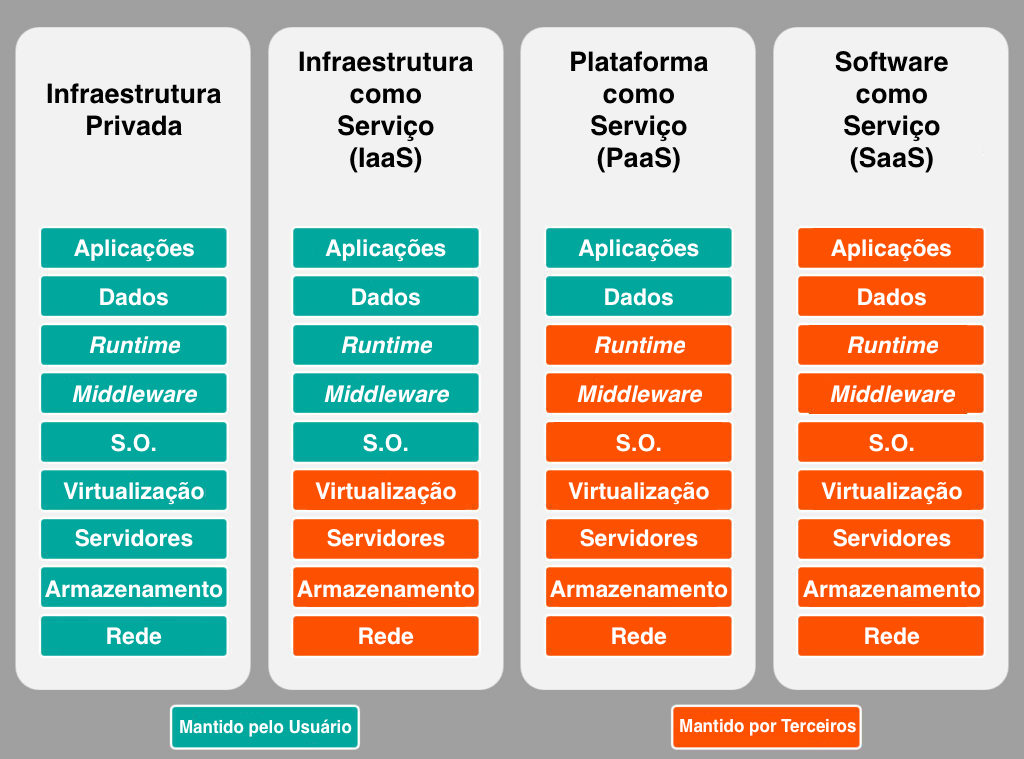
\includegraphics[width=14cm]{TCC/figuras/2-fundamentacao/ServiceModels}
    
	Fonte: Traduzido de \cite{servicemodelsimage}
 	\label{service_models}
\end{figure}

% ----------------------------------------------------------------------- %
\section{Sistemas Distribuídos}

De acordo com \citeonline{tanenbaum}, um sistema distribuído é um conjunto de computadores independentes que se apresenta a seus usuários como um sistema único e coerente. Entre as vantagens na utilização de sistemas distribuídos destacam-se a escalabilidade e redundância do sistema, que permitem que o sistema atenda à diversas aplicações e usuários. A contrapartida é a complexidade em seu gerenciamento, haja vista que o gerenciamento de recursos e dimensão do sistema ficam mais complexos.

Para que o sistema se apresente ao usuário como um sistema distribuído é necessário que ele cumpra quatro metas fundamentais \cite{tanenbaum}:

\begin{itemize}
    \item Acesso a recursos: o acesso a recursos do sistema deve ser eficiente e seguro.
    \item Transparência da distribuição: o sistema deve se apresentar ao usuário sendo como um único sistema, mesmo estando distribuído entre diversos computadores (por exemplo, ao acessar uma página \textit{Web} o usuário não possui conhecimento sobre qual servidor está de fato acessando).
    \item Abertura: ``um sistema distribuído aberto é um sistema que oferece serviços de acordo com regras padronizadas que descrevem a sintaxe e semântica desses serviços''  \cite{tanenbaum}.
    \item Escalabilidade: um sistema distribuído pode ser escalável em relação a seu tamanho (com adição de usuários e recursos ao sistema), termos geográficos (usuários e recursos podem estar longes uns dos outros) e administrativos (facilidade de gerenciamento) \cite{tanenbaum}.
\end{itemize}

Sistemas de computação distribuídos são classificados em dois subgrupos, sendo estes subgrupos os sistemas de computação em \textit{cluster} e em \textit{grid} \cite{tanenbaum}. Um \textit{cluster} consiste em um conjunto de computadores de \textit{hardware} semelhante interconectados entre si por uma rede de alta velocidade e que trabalham conjuntamente para executar tarefas que requerem alto poder computacional \cite{cluster&grid}. Já na computação em \textit{grid} o \textit{hardware} das estações é heterogêneo e as estações que compõem o sistema podem ser de diferentes organizações \cite{tanenbaum}. Em sistemas de computação em \textit{grid} a estratégia empregada para coordenação entre as estações é a utilização de um \textit{middleware} que divide e distribui tarefas entre os computadores \cite{cluster&grid}.

Como é possível perceber, é necessário que os computadores que fazem parte do sistema distribuído estejam altamente coordenados para realizar a computação de forma eficiente. Diversos modelos de coordenação são utilizados, como o Linda, o \textit{publish/subscribe} e o Jini \cite{tanenbaum2}. 

\subsection{Virtualização de Sistemas Operacionais}

Com o crescimento de volumes de dados e de serviços fornecidos através de redes \ac{IP} têm se evidenciado que a virtualização de infraestruturas provê melhor flexibilidade, custo, escalabilidade, utilização de recursos e eficiência energética em \textit{data centers} \cite{bari}. Até recentemente, a virtualização neste contexto significava apenas virtualização em \textit{hardware} através da execução de máquinas virtuais \cite{tay}, apesar do conceito de virtualização ser discutido e pesquisado há mais de 40 anos \cite{pearce}. Segundo \citeonline{walters}, a virtualização de sistemas operacionais pode ser majoritariamente categorizada em quatro grupos: virtualização total ou completa,  paravirtualização, virtualização em nível de sistema operacional e virtualização assistida por \textit{hardware}. Estes tipos de virtualização são explicados a seguir.

\subsubsection{Tipos de Virtualização de Sistema Operacional}

\begin{itemize}
    \item Virtualização total ou completa (\textit{Full Virtualization}): Também chamada de emulação de \textit{hardware}. Nesta categoria, o \textit{hypervisor} (\textit{software}, \textit{firmware} ou \textit{hardware} que encapsula e roda o sistema operacional emulado) provê as mesmas entradas, saídas e comportamentos que seriam esperados de um \textit{hardware} específico \cite{pearce}. De forma simples, o sistema operacional emulado não possui conhecimento de que está sendo virtualizado, e sim de que está sendo executado diretamente em \textit{hardware}. Este tipo de virtualização é computacionalmente intensivo e possui alto custo, pois o sistema operacional emulado não possui conhecimento de que está na verdade acessando um \textit{hardware} emulado pelo \textit{hypervisor}, o qual captura as exceções de acesso ao \textit{hardware} do sistema emulado e as emula de acordo com as configurações do \textit{hardware} emulado;
    \item Paravirtualização (\textit{Paravirtualization}): Na paravirtualização propõe-se que o sistema operacional virtualizado saiba que está sendo executado na camada virtual e interaja com a mesma. Isso implica a alteração do sistema operacional virtualizado, mas garante uma grande cooperação entre as duas camadas \cite{grosmann};
    \item Virtualização em nível de Sistema Operacional (\textit{Operating System-level Virtualization}): De forma simples, esta técnica de virtualização permite que recursos possam ser isolados dentro de um sistema operacional para execução de instâncias de espaços de usuários e aplicações, sendo o gerenciamento destes recursos realizados pelo sistema operacional, e não por um \textit{hypervisor}, o que aumenta o desempenho dessas instâncias \cite{walters};
    \item Virtualização Assistida por \textit{Hardware} (\textit{Hardware-Assisted Virtualization}): Esta técnica de virtualização consiste em uma virtualização total mas com auxílio em \textit{hardware} do processador, permitindo que as instruções da máquina virtual não sejam executadas em um processador emulado pelo \textit{hypervisor}, e sim diretamente no processador da máquina real \cite{walters}.
\end{itemize}

\subsection{Virtualização de Redes}

A virtualização de servidores sozinha não é suficiente para resolver os problemas e limitações de grandes infraestruturas, tais como os riscos de segurança ocasionados pela não-restrição de protocolos de comunicação utilizados por máquinas reais, as quais podem estar executando diversas máquinas virtuais simultaneamente \cite{bari}. Neste contexto, técnicas de virtualização de rede também têm sido aplicadas com o objetivo de solucionar alguns destes problemas e melhorar a performance e segurança do sistema. Técnicas como a utilização de \ac{VLANs} são as mais tradicionais em termos de virtualização, pois permitem que sejam criadas redes locais virtuais, restringindo assim o domínio de \textit{broadcast} de cada dispositivo e possibilitando a resolução de diversos dos problemas de \textit{data centers} \cite{bari}.
Com a utilização de técnicas de virtualização de rede torna-se fundamental a organização de uma topologia que facilite a implementação e manutenção da rede. Ao definir a topologia de uma rede, é importante definir se ela será escalável horizontalmente ou verticalmente. A escalabilidade horizontal refere-se a adicionar nós no sistema, o que permite a distribuição de carga de trabalho a múltiplas máquinas e a utilização de \textit{hardware} heterogêneo no sistema \cite{gregol}. Já a escalabilidade vertical refere-se a melhorar o sistema ao adicionar mais recursos a um nó, tais como aumentar a memória ou capacidade de armazenamento do mesmo \cite{barzu}. A \autoref{datacenter_topology} exibe a topologia convencional de \textit{data center} segundo \citeonline{barzu}.

\begin{figure}[!htpb]
	\centering
	\caption{Topologia convencional de um \textit{data center}}
    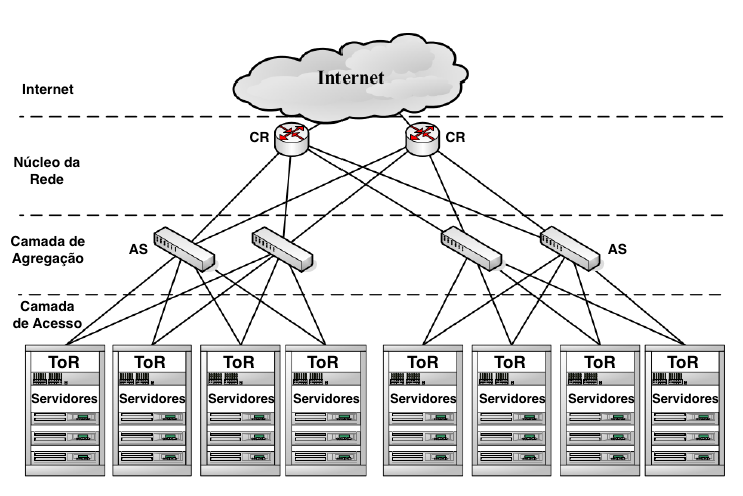
\includegraphics[width=13cm]{TCC/figuras/2-fundamentacao/DCNetworkConventional}
    
	Fonte: Traduzido de \cite{bari}
 	\label{datacenter_topology}
\end{figure}

Como exibido na \autoref{datacenter_topology}, esta topologia é convencionalmente horizontal, pois permite que diferentes dispositivos de uma mesma categoria (\textit{switches}, roteadores e servidores) sejam adicionados ao sistema, evitando assim a necessidade de utilizar tecnologias proprietárias e altos custos na melhoria do sistema, por exemplo. É importante ressaltar que nem sempre esta solução é a ideal, pois ocorrem casos em que melhorar um nó individual é mais efetivo do que adicionar nós ao sistema. Por exemplo, pode ser mais efetivo melhorar a capacidade de processamento de um nó para fornecimento de um serviço específico do que adicionar nós ao sistema. Na topologia apresentada na \autoref{datacenter_topology}, o \textit{switch} \ac{ToR} realiza a conexão entre os servidores montados em um mesmo \textit{rack}, enquanto os \textit{switches} de agregação (\ac{AS}) encaminham o tráfego dos \textit{switches} \ac{ToR} para os roteadores do núcleo da rede (\ac{CR}) \cite{bari}. É importante ressaltar a redundância entre os \textit{switches} \ac{ToR} e de agregação, que garantem que o sistema continuará em operação em caso de falhas pontuais. Esta topologia é denominada topologia \ac{ToR} (referenciando o \textit{switch} \ac{ToR}, componente vital do sistema).

\subsection{Contêineres}

Os avanços no \textit{kernel} do Linux levaram ao desenvolvimento de isolamento de recursos baseado em contêineres \cite{containersXvms}. De forma simples, um contêiner pode ser definido como um pacote executável de um \textit{software} que inclui tudo o que é necessário para executar este \textit{software}: código, bibliotecas, configurações, ferramentas, entre outros \cite{aboutcontainer}. 

Contêineres e máquinas virtuais são soluções distintas para problemas distintos. De acordo com \citeonline{paascontainer}:

\begin{citacao}
``[...] \textit{contêineres são ferramentas para prover software - isto é, seu foco é na entrega de uma PaaS - com grande portabilidade e interoperabilidade enquanto utilizando técnicas de virtualização. Por outro lado, máquinas virtuais se preocupam com alocação e gerenciamento de hardware - isto é, seu foco é na entrega de uma IaaS que fornece serviços através da virtualização de hardware}.''
\end{citacao}

Existem diferentes tecnologias de contêineres, sendo o Docker uma das tecnologias que está se tornando uma das mais utilizadas para criação de contêineres \cite{openstackContainer}. O Docker é uma ferramenta que facilita a criação e distribuição de contêineres com suas dependências \cite{containers&docker}, sendo um projeto de código aberto que possui mais de 3 mil colaboradores \cite{aboutdocker}. A \autoref{virtualization_layers} exibe a abstração das camadas de máquinas virtuais e contêineres Docker. É possível perceber que, diferentemente de máquinas virtuais, contêineres não requisitam que seja realizada a virtualização completa de um sistema operacional. A vantagem desta abordagem é de que não há duplicação de funcionalidades, como por exemplo chamadas de \textit{hardware}, já que apenas um sistema operacional lida com todo o acesso ao \textit{hardware} \cite{containers&docker}.

\begin{figure}[!htpb]
	\centering
	\caption{Comparação entre máquinas virtuais e contêineres}
    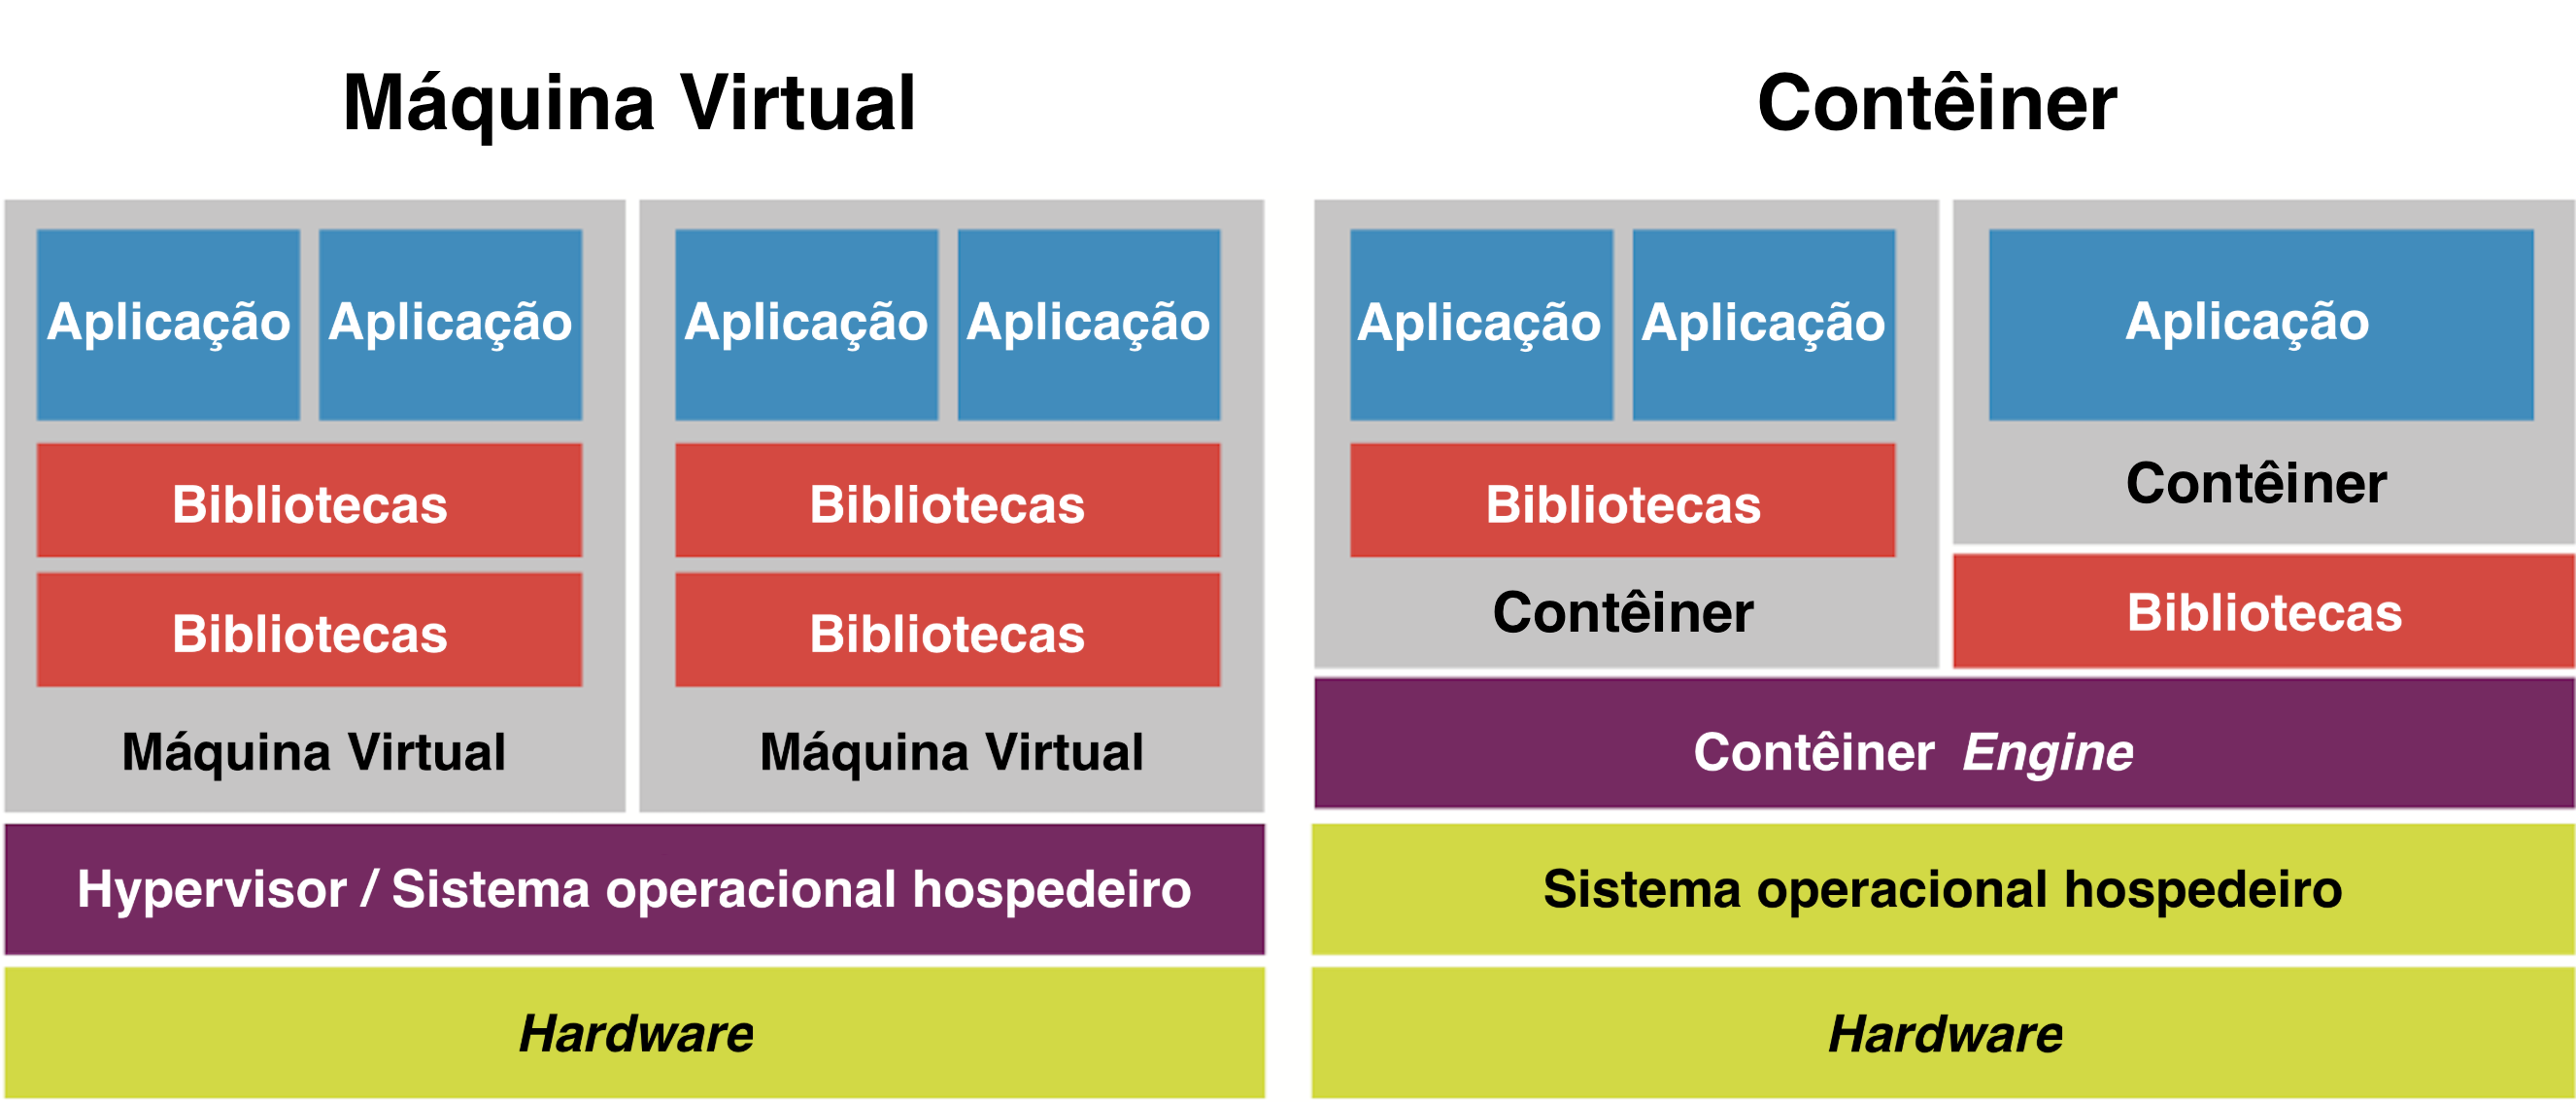
\includegraphics[width=13cm]{TCC/figuras/2-fundamentacao/Virtualization}
    
	Fonte: Traduzido de \cite{paascontainer}
 	\label{virtualization_layers}
\end{figure}

Como contêineres - diferentemente de máquinas virtuais - rodam como processos em um mesmo sistema operacional, é possível (e necessário) restringir e limitar o acesso a recursos do sistema operacional hospedeiro. Para contêineres em Linux, o controle ao acesso de recursos é realizado através de \textit{namespaces} e grupos de controle (\textit{cgroups}) \cite{containers&docker}. \textit{Namespaces} permitem que grupos de processos sejam separados, evitando assim que estes processos acessem recursos de outros grupos \cite{paascontainer}. Grupos de controle permitem o gerenciamento de recursos por grupos de processos, possibilitando que o uso de memória seja limitado para um grupo, por exemplo \cite{paascontainer}.

Segundo \citeonline{containersXvms}, quatro são as características que tornam contêineres úteis e atrativos no desenvolvimento de aplicações e fornecimento de serviços:

\begin{itemize}
    \item Portabilidade: aplicações podem ser desenvolvidas em um ambiente e ser implantadas em diversos outros ambientes sem necessidade de alterar o contêiner.
    \item Rapidez na entrega da aplicação: o fluxo de desenvolvimento de contêineres permite que administradores de sistema, desenvolvedores e equipe de testes efetuem a implantação da aplicação rapidamente, pois apenas os desenvolvedores precisam se preocupar com o formato e conteúdo do contêiner e os administradores de sistema com sua implantação nos servidores.
    \item Escalabilidade: a escalabilidade vertical e horizontal de contêineres 
    é muito mais rápida do que a de máquinas virtuais, já que os recursos utilizados pelos contêineres são oferecidos nativamente pelo sistema operacional, sem necessidade de virtualização de chamadas de \textit{hardware}.
    \item Maior carga de trabalho e densidade: como não é necessário utilizar um \textit{hypervisor} para virtualização, é possível executar uma quantidade maior de contêineres do que de máquinas virtuais concorrentemente. Além disso, o processamento está concentrado na aplicação, sem necessidade de virtualização de chamadas de \textit{hardware}, como no caso de máquinas virtuais, por exemplo.
\end{itemize}

Após a criação do contêiner, é possível gerenciá-lo utilizando uma ferramenta de orquestração de contêineres, que permite a criação de \textit{clusters} de contêineres e seu gerenciamento.

\subsubsection{Orquestração de Contêineres}

De acordo com \citeonline{containerOrchestration}, uma plataforma de orquestração de contêineres pode ser, de forma geral, definida como um sistema que provê um \textit{framework} para integração e gestão de contêineres em larga escala.  Estas plataformas simplificam a gestão de contêineres e fornecem um \textit{framework} para não apenas realizar a implantação inicial de contêineres mas também a gestão de múltiplos contêineres como uma entidade, seja para propósitos de escalabilidade ou disponibilidade, por exemplo. Como exemplos de orquestradores de contêineres populares pode-se citar o Docker Swarm e o Kubernetes, enquanto  \ac{GKE}, \ac{Amazon EKS} e \ac{AKS} são implementações do orquestrador Kubernetes em nuvens públicas.

\subsubsubsection{Kubernetes}

Kubernetes é uma plataforma de código aberto para orquestração de contêineres a qual facilita tanto configurações declarativas e automatizações. Disponibilizada em 2014 e criada pela Google, hoje a plataforma é mantida pela \ac{CNCF} \cite{aboutkubernetes}.

Um \textit{cluster} Kubernetes consiste em dois tipos de recursos: mestres e nós. A interligação entre estes recursos coordenados por um mesmo orquestrador Kubernetes é denominado \textit{cluster} \cite{minikubeCluster}. Os mestres são responsáveis por coordenar o \textit{cluster}, enquanto os nós são as unidades que de fato executam as aplicações do \textit{cluster}, as quais são implantadas através de contêineres. A \autoref{k8sArchitecture} mostra a arquitetura básica de um \textit{cluster} Kubernetes.

\begin{figure}[!htpb]
	\centering
	\caption{Arquitetura de \textit{cluster} Kubernetes}
    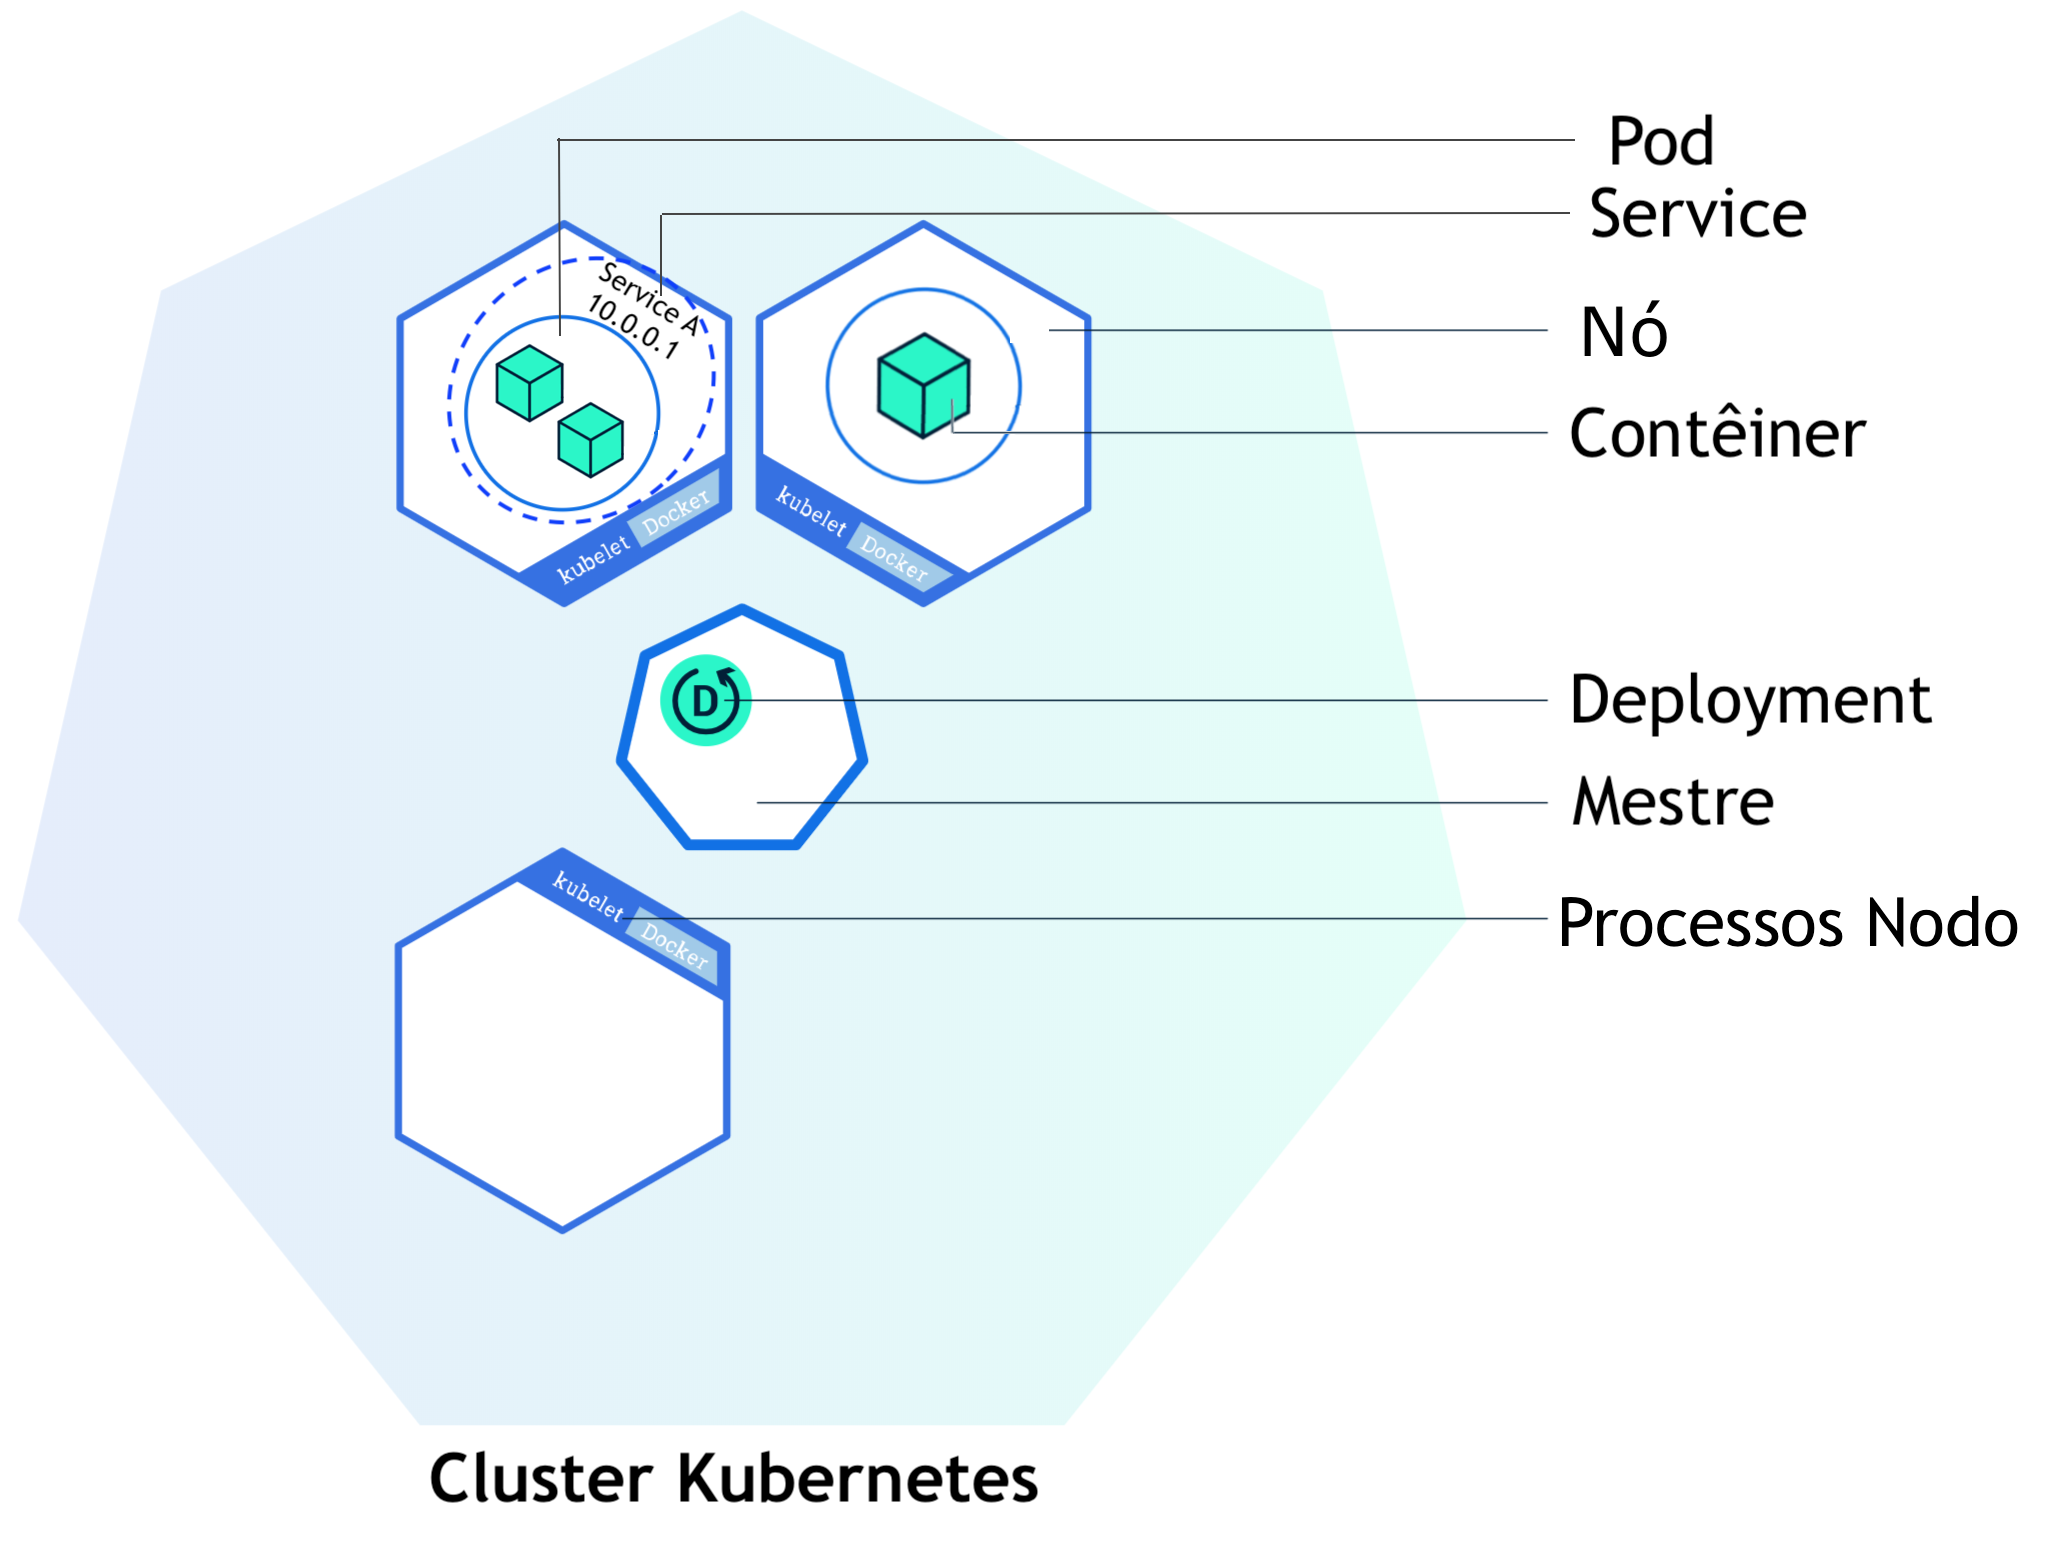
\includegraphics[width=13cm]{TCC/figuras/2-fundamentacao/K8s-architecture}
    
	Fonte: Adaptado de \cite{minikubeCluster}
 	\label{k8sArchitecture}
\end{figure}

Na aquitetura da \autoref{k8sArchitecture} há um mestre e três nós. Os \textit{pods}, \textit{deployments} e \textit{services} são entidades persistentes do sistema Kubernetes e são tratados como objetos \cite{kubernetesObjects}. Já o processo \textit{kubelet} é o ``agente'' que roda no nó para que este faça parte do \textit{cluster} \cite{kubernetesKubelet}.

Um \textit{pod} é um grupo de um ou mais contêineres que compartilham armazenamento, rede e outros recursos computacionais e especifica como executar estes contêineres. Assim como contêineres, \textit{pods} são isolados através da utilização de \textit{namespaces} linux, \textit{cgroups} e outras formas de isolamento. \textit{Pods} podem ser utilizados para implantar \textit{proxies} e ferramentas de monitoramento, por exemplo \cite{kubernetesPods}.

\textit{Services} são uma abstração que definem as políticas de acesso a \textit{pods}. \textit{Pods} podem ser expostos através de diferentes tipos de \textit{services}, havendo desde \textit{services} que expõem uma porta do nó externamente ao \textit{cluster} (\texttt{NodePort}) até \textit{services} que limitam o acesso ao \textit{pod} a endereços \ac{IP} internos ao \textit{cluster} (\texttt{clusterIP}) \cite{kubernetesServices}.

Já um \textit{deployment} permite que \textit{pods} sejam criados e atualizados através de linguagem declarativa. \textit{Deployments} fornecem um mecanismo de auto-reparação que permite que \textit{pods} sejam reiniciados caso falhas ocorram, por exemplo \cite{kubernetesDeployments}.

Outros componenentes do Kubernetes que também merecem destaque são o \textit{StorageClass} e o \textit{Ingress}. De forma simples, uma \textit{StorageClass} é uma classe que descreve como o armazenamento através de volumes persistentes (\ac{PV}) será provido a aplicações \cite{kubernetesStorageClass}. Esta abordagem é vantajosa pois permite que diferentes \textit{StorageClasses} com diferentes características possam ser criados no \textit{cluster} Kubernetes, permitindo assim que a aplicação utilize a que melhor se adeque as suas necessidades. Para utilização de um volume é necessário que um \textit{pod} solicite a criação deste volume através de uma requisição de volume persistente (\ac{PVC}), a qual será processada pelo \textit{Storage Class}.

Já o \textit{Ingress} é um recurso do Kubernetes que atua na camada de aplicação da arquitetura \ac{TCP}/\ac{IP} e permite a criação de regras de acesso a serviços do \textit{cluster} através de domínios ou recursos personalizados, além de também possibilitar o balanceamento de carga e implementação de criptografia no acesso a estes serviços. Um \textit{Ingress} consiste, portanto, de um conjunto de regras que permitem que o tráfego de entrada possa acessar os serviços do \textit{cluster} \cite{kubernetesIngress}. É importante ressaltar que aprimoramentos estão sendo realizados para possibilitar que a camada de transporte também seja controlada através do \textit{Ingress}, mas esta funcionalidade ainda está em desenvolvimento \cite{ingressTCPUDP}.

Outros objetos, tais como \textit{ReplicaSets} e \textit{ResourceQuotas} também são vastamente utilizados em \textit{clusters} Kubernetes. Também é possível criar definições de recursos customizados (\ac{CRD}) através da \ac{API} do Kubernetes para que novos objetos possam ser utilizados. A \autoref{k8schematic} exemplifica a organização dos objetos \textit{Deployment}, \textit{ReplicaSet}, \textit{Pod}, \ac{PVC}, \ac{PV}, \textit{StorageClass}, \textit{Service} e \textit{Ingress Controller} na implantação de uma aplicação em um \textit{cluster} Kubernetes.

\begin{figure}[!htpb]
	\centering
	\caption{Objetos do Kubernetes}
    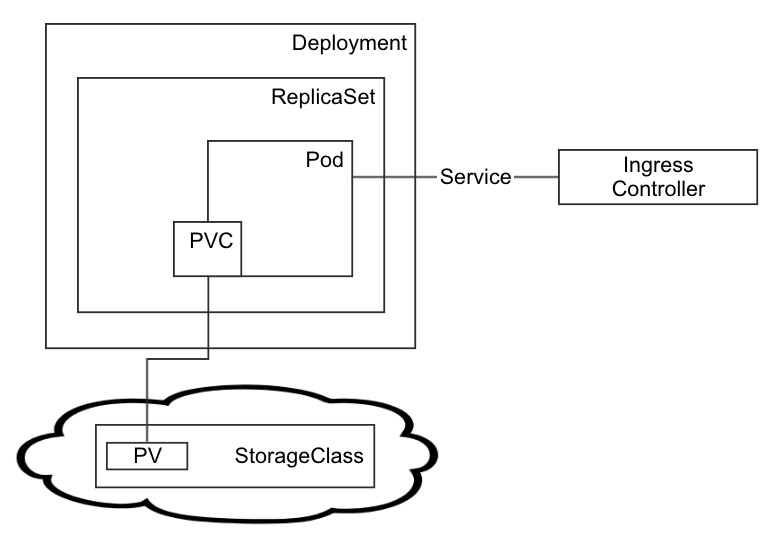
\includegraphics[width=13cm]{TCC/figuras/2-fundamentacao/k8s-complete-schematic.png}
    
	Fonte: Elaborado pelo autor.
 	\label{k8schematic}
\end{figure}

\subsubsubsection{Helm}

O Helm é um gerenciador de pacotes para Kubernetes \cite{abouthelm}. Estes pacotes são denominados \textit{charts} e podem ser instalados em um \textit{cluster} Kubernetes a partir de repositórios públicos ou privados, dispensando assim a necessidade de criar todos os recursos necessários para a implantação de uma aplicação manualmente.

Um \textit{chart} Helm pode, por exemplo, implantar uma aplicação WordPress em um \textit{cluster} de forma automatizada, criando de forma automatizada os \textit{Deployments}, \textit{Services} e \textit{ReplicaSets} necessários para implantacão da aplicação.

\subsubsection{Rancher}

Assim como o Kubernetes é uma ferramenta para orquestração de contêineres, o Rancher é uma plataforma para administração de \textit{clusters} Kubernetes. Ele facilita, por exemplo, o monitoramento dos recursos de \textit{clusters} e criação e manutenção de \textit{clusters} híbridos \cite{rancherOverview}.

A arquitetura em alto nível do Rancher é simples: é necessário apenas a criação de um servidor para gerenciamento dos \textit{clusters} e configurar a conexão e permissões de acesso do Rancher a estes \textit{clusters}. Também é possível utilizar a ferramenta de gerenciamento \ac{RKE} para rápida criação de \textit{clusters} Kubernetes.

% ----------------------------------------------------------------------- %
\section{Sistemas de Arquivos}

De acordo com \citeonline{tanenbaum2}, a parte do sistema operacional que trata do modo como os arquivos são estruturados, nomeados, acessados, usados, protegidos e implementados é o sistema de arquivos. Exemplos de sistemas de arquivos são o ISO 9660 (utilizado em CD-ROMs), FAT-32 (extensão do sistema de arquivos MS-DOS da Microsoft) e EXT4 (evolução do sistema de arquivos EXT3 do Linux). 

\subsection{Sistemas de Arquivos Distribuídos}

Segundo \citeonline{authdfs}, um sistema de arquivos distribuído é um sistema no qual os arquivos estão armazenados e distribuídos em computadores diferentes interligados por meio de uma rede de comunicação. Um sistema de arquivos distribuído apresenta o mesmo conceito de um sistema de arquivos local, ou seja, ele também trata do gerenciamento de arquivos, porém no contexto distribuído. Ele permite, portanto, que usuários e programas remotos leiam e escrevam dados que estão aparentemente armazenados na máquina do usuário, mas que na verdade estão disponíveis remotamente. Isto significa, portanto, que ele cumpre a meta fundamental de ser um sistema transparente ao usuário.

Além das vantagens inerentes de rápida escalabilidade e maior redundância do sistema distribuído, sistemas de arquivos distribuídos também podem oferecer a vantagem de fornecer acesso a uma base unificada de dados aos usuários, evitando réplicas desnecessárias de arquivos em máquinas locais. Entretanto, uma desvantagem que merece destaque na utilização de sistemas de arquivos distribuídos é a necessidade de uma boa infraestrutura de rede para suportar o constante tráfego de arquivos, que pode ser ineficiente em uma rede precária e de baixas taxas de transmissão.

Exemplos de sistemas de arquivos distribuídos são o Ceph, GlusterFS, StorageOS, \ac{GFS} e Lustre. Dos exemplos citados apenas o primeiro será objeto de estudo deste trabalho, pois a implementação deste sistema de arquivos em Kubernetes têm recebido grande apoio da \ac{CNCF} \cite{rookincubator}.

\subsubsection{Ceph}

Ceph é um sistema de armazenamento distribuído de código aberto. Este sistema de armazenamento permite que dados sejam armazenados não apenas no formato de arquivos, mas também como blocos e objetos \cite{cephdocumentation}.

O armazenamento através de arquivos ocorre quando os dados são salvos em uma única quantidade de armazenamento, geralmente organizada por diretórios. Já o armazenamento em blocos ocorre quando o armazenamento disponível é dividido em blocos e estes blocos podem ser utilizados por diferentes aplicações, seja de forma distribuída ou não. Finalmente, o armazenamento através de objetos é uma estrutura horizontal onde dados são armazenados como uma unidade denominada objeto e possuem um identificador único que localiza este objeto na estrutura de dados. Este identificador é salvo em um servidor de metadados, que também pode armazenar informações como data de criação do objeto e permissões de acesso, por exemplo \cite{redhatStorage}.

O Ceph foi projetado sob a premissa de que grandes sistemas de armazenamento de dados possuem o potencial de armazenar ainda mais informações, e falhas de componentes não são exceções, e sim constantes \cite{cephFailures}. Assumir que falhas de componentes são comuns no sistema e trabalhar para contornar estas falhas torna o Ceph um sistema poderoso.

Uma das características mais interessantes do Ceph é o algoritmo \ac{CRUSH}. O \ac{CRUSH} é um algoritmo de locação pseudo-randômico que permite que clientes possam computar a localização de um dado no \textit{cluster} sem precisar consultar uma tabela central que guarde a localização de todos os dados do \textit{cluster}. Como consequência, o Ceph busca garantir a escalabilidade e confiabilidade do sistema através da computação inteligente dos dados nele armazenados \cite{cephPerformance}.

Cinco são os componentes principais de um \textit{cluster} Ceph: \ac{OSD}s, \textit{Monitors}, \textit{Managers}, \ac{MDS} e \ac{RADOS}. Cada um destes componentes é explicado a seguir:

\begin{itemize}
    \item \ac{OSD}s: um \ac{OSD} armazena dados, processa replicação de dados e fornece informações de monitoramento para os \textit{Monitors} e \textit{Managers} \cite{aboutceph}. Estes são os componentes de ``mais baixo nível'' do \textit{cluster} Ceph.
    \item \textit{Monitors}: mantém mapas e informações do \textit{cluster}, tais como mapa de outros \textit{Monitors}, \ac{OSD}s e \textit{Managers} existentes, além do mapa \ac{CRUSH} utilizado para computação da localização dos dados armazenados \cite{aboutceph}. \textit{Monitors} também são responsáveis pela autenticação de clientes e \textit{daemons}. Quando um cliente deseja armazenar ou acessar dados do \textit{cluster} ele deve se conectar ao \textit{Monitor} para se autenticar e obter o mapa do \textit{cluster} e, após ser devidamente autenticado, ele poderá conectar-se diretamente o \ac{OSD} correspondente para realizar a operação desejada \cite{cephArchitecture}.
    \item \textit{Managers}: os \textit{Managers} são responsáveis por registrar métricas de execução e estado do \textit{cluster} Ceph, além da carga de trabalho do sistema. Os \textit{Managers} permitem a consulta de métricas do sistema através de \textit{plugins} como uma \textit{dashboard} (painel de controle) e uma \ac{REST} \ac{API} \cite{aboutceph}.
    \item \ac{MDS}s: armazenam metadados do sistema de arquivos Ceph, como permissões e propriedades de arquivos, ou seja, se o Ceph for utilizado como armazenamento em blocos ou objetos \ac{MDS}s não serão necessários \cite{aboutceph}.
    \item \ac{RADOS}: consiste na junção de \ac{OSD}s e \textit{Monitors} para distribuição de dados como objetos pelo \textit{cluster} e replicação de dados \cite{openstackCephBlock}. O \ac{RGW} é uma interface que fornece uma \ac{REST} \ac{API} para acesso aos objetos armazenados pelo \ac{RADOS}. Esta \ac{API} é compatível com as interfaces S3 da Amazon e OpenStack Swift \cite{cephRadosGW}.
\end{itemize}

\subsubsection{Rook}

O Rook é um projeto de código aberto incubado pela \ac{CNCF} \cite{rookincubator}. De forma simples, o Rook é um orquestrador de armazenamento para \textit{clusters} Kubernetes que automatiza a implantação do Ceph nestes sistemas. No presente momento (segundo semestre de 2018) a implementação do Ceph através do Rook está em estado Beta \cite{rookdocumentation}.

O Rook permite, por exemplo, que sejam automaticamente implantados todos os \ac{OSD}s necessários em nodos específicos, dispensando assim a necessidade de manualmente instalar e configurar os \textit{daemons} necessários nestes nodos. Assim como o Ceph, é possível utilizar o Rook para orquestrar o armazenamento de dados através de arquivos, blocos e objetos.

O armazenamento através de blocos pode ser empregado no Rook através da implantação de uma \textit{Storage Class} do Rook via \ac{CRD}. Já o armazenamento de objetos pode ser realizado através de uma \textit{Object Store}, a qual - assim como o \ac{RADOS} do Ceph - oferece uma \ac{REST} \ac{API} para acesso aos objetos armazenados. Já um sistema de arquivos distribuído pode ser implantado no Rook através de um \textit{Shared File System}, o qual também pode ser associado a serviços como um volume.

A maior parte dos componentes criados pelo Rook no \textit{cluster} são componentes equivalentes aos do Ceph. Um \textit{pod} \ac{OSD} do Rook, por exemplo, também possui como função armazenar os dados em disco e prover acesso a estes dados para outros programas.


\subsection{Convergência de infraestrutura}

Uma \ac{CI} é a convergência das infraestruturas de computação, armazenamento e rede em um \textit{data center} \cite{netappconvergence}. A \ac{CI} almeja alcançar o melhor desempenho do sistema com padronização dos protocolos e \textit{hardware} utilizado no \textit{data center}, muitas vezes através da utilização de \textit{hardware} proprietário que realize funções específicas \cite{netappconvergence}.
 
Uma \ac{HCI} é uma infraestrutura definida por \textit{software} que pode ser dimensionada horizontalmente \cite{vmwarehyperconvergence} e que combina computação, virtualização, armazenamento e rede em um único \textit{cluster} \cite{ciscohyperconvergence}. A hiperconvergência traz simplicidade a \textit{clusters} locais com uma única e simples plataforma de computação e gerenciamento. Com a \ac{HCI}, todas as principais funções do \textit{data center} são executadas em uma camada de \textit{software} altamente integrada, simplificando o fornecimento de serviços que antes exigiam \textit{hardware} específico para uma finalidade. Dentre as vantagens oferecidas pela hiperconvergência encontram-se a simplicidade de administração do sistema e o baixo custo total de propriedade \cite{vmwarehyperconvergence}. Como a proposta de uma infraestrutura hiperconvergente consiste na combinação das infraestruturas de computação, virtualização, armazenamento e rede em um único \textit{cluster}, é possível alcançar este modelo através de uma infraestrutura de contêineres, que pode combinar todas as infraestruturas através de uma única plataforma de gerenciamento. A \autoref{hcischematic} mostra que armazenamento, rede e computação podem ser combinados através da utilização de contêineres, sendo o armazenamento implementado através do \textit{StorageClass}, a rede através de \textit{Services} e recursos \textit{Ingress} (gerenciados pelo \textit{Ingress Controller}) e a computação através dos \textit{Pods}, \textit{Deployments} e \textit{ReplicaSets}.

\begin{figure}[!htpb]
	\centering
	\caption{Infraestrutura hiperconvergente de contêineres}
    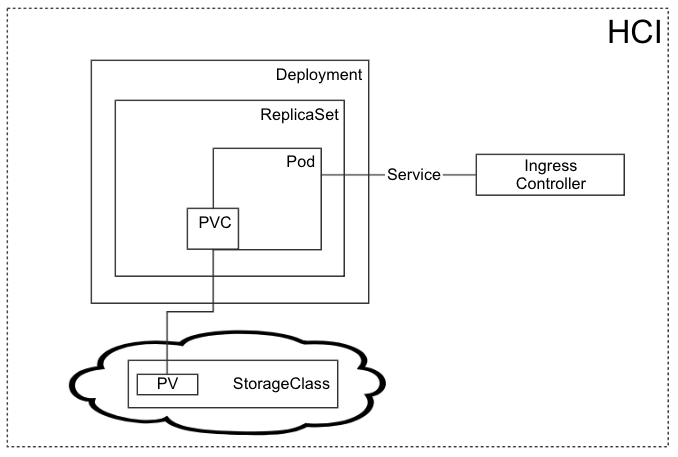
\includegraphics[width=11cm]{TCC/figuras/2-fundamentacao/hci-container.png}
    
	Fonte: Elaborado pelo autor.
 	\label{hcischematic}
\end{figure}
% % ----------------------------------------------------------------------- %
% % Arquivo: 3-cenario-IFSC.tex
% % ----------------------------------------------------------------------- %

% \chapter{Estudo de Caso: Infraestrutura de Serviços do IFSC}
% \label{c_cenario}

% Após conversas com servidores da \ac{CTIC} do \ac{IFSC} câmpus São José e pesquisas realizadas em documentos disponíveis em portais da instituição percebeu-se que há um movimento emergente em setores do \ac{IFSC} para implantação de políticas de \ac{TI} eficientes e condizentes com a realidade da instituição. Há também discussões sobre os serviços atualmente fornecidos por cada câmpus da instituição e sobre como melhorar a disponibilidade e eficiência dos serviços oferecidos através do \textit{data center} mantido pela Reitoria do \ac{IFSC}, onde a infraestrutura de serviços da instituição é centralizada.

% Por este motivo, é necessário contextualizar o presente estado das políticas de \ac{TI} e infraestrutura do \ac{IFSC} para que o sistema distribuído proposto neste trabalho possa ser melhor entendido e justificado. A seguir é feita uma discussão sobre as políticas de \ac{TI} do \ac{IFSC}, os pontos positivos da centralização da infraestrutura e as deficiências do modelo de infraestrutura adotados pela instituição.

% % ----------------------------------------------------------------------- %
% \section{Política de TI do IFSC}

% Nos últimos anos o \ac{IFSC} tem se preocupado com suas políticas de governança de \ac{TI}. Em 2015, por exemplo, diversas normas e políticas foram adotadas pelo \ac{IFSC} em relação ao uso de recursos pelos discentes e docentes dos câmpus da instituição \cite{dticpoliticas}. Em 2017 foi criada a Coordenadoria de Governança de \ac{TI}, responsável por responder pelos processos de compras de \ac{TI}, planejamento e governança \cite{pdti2018}. A estrutura organizacional atual da \ac{TIC} do \ac{IFSC} é exibida na \autoref{organizacaoIFSC}, e a descrição das funções de cada departamento é descrita na Resolução CONSUP nº 12, de 24 de abril de 2017 \cite{pdti2018}.

% \begin{figure}[!htpb]
% 	\centering
% 	\caption{Estrutura institucional da TIC do IFSC}
%     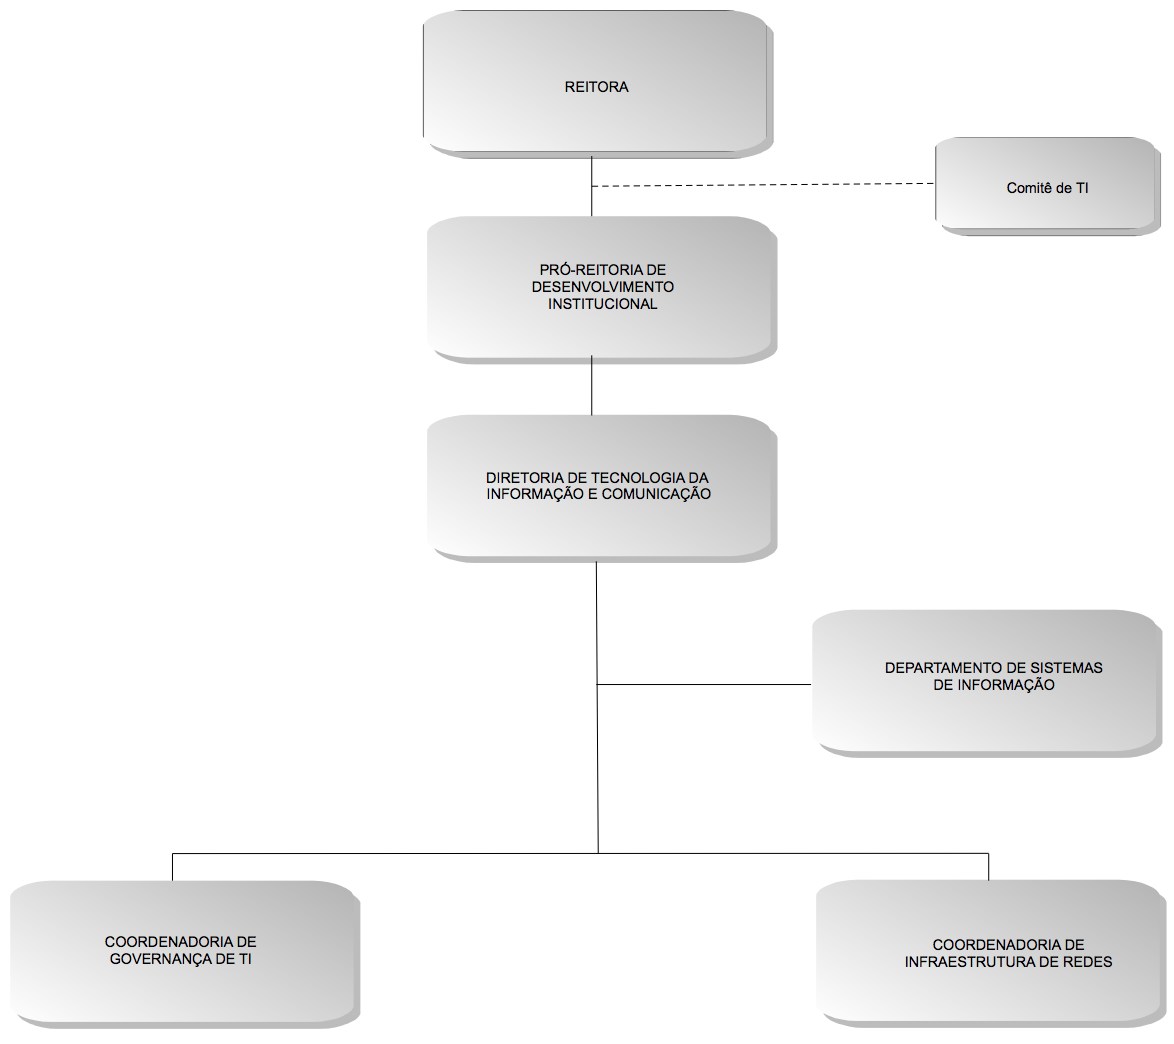
\includegraphics[width=15cm]{TCC/figuras/3-cenario/OrganogramaIFSC}
    
% 	Fonte: Extraído de \cite{pdti2017}
%  	\label{organizacaoIFSC}
% \end{figure}

% Embora haja esforço para estabelecimento de novas políticas, normas e procedimentos de \ac{TI} dentro da instituição, ainda há muito a ser feito. A \ac{UFSC}, por exemplo, já possui suas políticas e procedimentos de \ac{TI} definidos e em constante aprimoramento. A instituição já está ofertando acesso a serviços em nuvem à comunidade acadêmica \cite{seticNuvem} e possui um portal público onde são registradas manutenções na rede e em serviços ofertados à comunidade acadêmica \cite{seticUFSC}. Além disso, a matriz de responsabilidade da instituição define as responsabilidades atribuídas a membros da \ac{SeTIC}, o que também contribui com a transparência e organização do setor \cite{matrizUFSC}. O reconhecimento da organização e gestão dos setores de \ac{TI} da \ac{UFSC} é percebido no cálculo do perfil de governança de \ac{TI} da instituição, realizado pelo \ac{TCU}. Este índice vai de 0 a 1, sendo que quanto maior o índice, melhor a condução das políticas de \ac{TI} da instituição.  Em 2016 o índice alcançado pela \ac{UFSC} foi de 0,61 (intermediário), enquanto o índice obtido pelo \ac{IFSC} foi de 0,38 (básico) \cite{igovti}. A média das instituições avaliadas é de 0,49 com desvio padrão de 0,18.

% Existem iniciativas dentro da instituição para aumentar a transparência dos setores de \ac{TI}. A \ac{CTIC} do câmpus São José, por exemplo, já compartilha publicamente os códigos utilizados para manutenção e implantação de serviços \cite{github-sj} e também disponibiliza acesso a plataforma de gestão de seus projetos \cite{trello-sj}. A iniciativa do câmpus São José mostra como políticas de \ac{TI} e transparência são emergentes dentro da instituição. Entretanto, o interesse na implantação de tais políticas também deve partir de cargos de coordenadoria e de departamentos da alta hierarquia, os quais devem se preocupar com o cenário global de transparência e organização da instituição. É importante ressaltar que a implantação de políticas de \ac{TI} é um processo demorado e trabalhoso, mas que após a implantação de tais políticas a gestão de recursos da instituição é facilitada e mais eficiente. O \ac{GED}, por exemplo, é um tópico recorrente em cada edição do \ac{PDTI} desde 2011, sendo seu estado de execução constantemente descrito como \textit{em execução} {\color{blue}(IFSC, 2011, 2013, 2014, 2016, 2017, 2018b)}. Após implantado, o sistema de gestão de documentos eletrônicos deverá permitir acesso a cópias digitalizadas de todos os documentos da instituição, aumentando a transparência do \ac{IFSC} e facilitando o fornecimento de documentos ao público. É importante ressaltar que, de acordo com a Portaria nº 315, de 4 de abril de 2018, o \ac{IFSC} possui até abril de 2020 para converter para o meio digital os ``documentos e informações que compõem o acervo acadêmico, independente da fase em que se encontrem ou de sua destinação final'' \cite{portaria315}. Esta é, portanto, uma discussão que também é realizada em outras instituições de ensino.

% Espera-se que o sistema proposto neste trabalho juntamente com as propostas de infraestrutura da \ac{CTIC} do câmpus São José sejam não apenas implantados no futuro, mas que também tragam mais atenção a discussões referentes a governança e políticas de \ac{TI} dentro da instituição e resolvam algumas das deficiências do modelo atual.


% % ----------------------------------------------------------------------- %
% \section{Pontos Positivos do Modelo Atual}

% Entre os pontos positivos do modelo de infraestrutura de serviços atual do \ac{IFSC} encontram-se a facilidade na administração dos serviços ofertados e armazenamento de dados, os quais estão localizados em apenas um \textit{data center}.

% Também é importante ressaltar que os funcionários dos departamentos de \ac{TIC} dos câmpus do \ac{IFSC} possuem diferentes formações e especialidades. Logo, o modelo centralizado permite que os funcionários que possuam maior capacitação para manutenção do sistema possam estar concentrados nestas funções. Expandir a infraestrutura para outros câmpus significaria a necessidade de treinamento das equipes de \ac{TIC}, o que pode ser demorado e custoso para a instituição.

% O modelo centralizado e topologia vertical do sistema podem ser onerosos, mas a alta qualidade do \textit{hardware} utilizado fornece confiabilidade ao sistema. Além disso, as garantias e assistências técnicas contratadas para tal \textit{hardware} permitem que a manutenção de tais equipamentos sejam agilizada devido as especialidades das empresas de manutenção contratadas.

% O atual funcionamento do sistema permite também que novos serviços possam ser mais facilmente implementados, enquanto uma remodelagem do sistema resultaria em um grande movimento para migração de serviços e verificação de compatibilidade dos serviços atuais com uma nova infraestrutura.

% % ----------------------------------------------------------------------- %
% \section{Cenário Ideal}

% O cenário ideal de infraestrutura em nuvem do \ac{IFSC} consiste em uma infraestrutura de alta disponibilidade, baixo custo financeiro, alto poder de processamento, fácil manutenção e gerenciamento, e que possa ser futuramente integrada a outras nuvens e serviços externos a instituição. Também faz parte do cenário ideal a implementação de um \textit{data center} horizontal e distribuído, concentrando a redundância da infraestrutura em \textit{software} ao invés de em \textit{hardware}, dispensando assim dispositivos complexos e proprietários que tornem a instituição dependente de terceiros tanto na instalação quanto na manutenção destes dispositivos. Os aplicativos utilizados devem ser livres e utilizar padrões abertos, permitindo assim que sejam utilizados sem restrições de licenças e possam ser facilmente integrados com outras nuvens. Já a infraestrutura deve ser distribuída e possuir distribuição de carga na utilização e acesso de serviços e dados. Esta nuvem deve continuar oferecendo os serviços que já são oferecidos à comunidade acadêmica atual e implementar ainda mais serviços, como utilização remota de aplicativos disponíveis apenas nas unidades físicas da instituição, por exemplo. Todas estas características são sugeridas para que o \ac{IFSC} possua uma infraestrutura tolerante a falhas, eficaz e facilmente escalável, permitindo assim que a comunidade acadêmica seja amplamente atendida e não vivencie interrupções de serviços.

% Além destes requisitos também é necessário que os funcionários de \ac{TI} dos câmpus do \ac{IFSC} sejam capacitados para operar e manter este sistema, delegando assim funções específicas para  membros específicos do setor. Considerando que todos os serviços acadêmicos (tanto administrativos quanto de ensino) seriam migrados para esta infraestrutura, é necessário, portanto, que cada câmpus possua pelo menos um responsável pela manutenção da infraestrutura e serviços ofertados neste câmpus.

% Com a expansão da infraestrutura de serviços e aumento do poder de processamento do sistema também é possível oferecer a maior parte dos serviços utilizados pela instituição em nuvem, dispensando assim a necessidade de utilização de aplicativos que necessitem de processamento local, fato que possibilitaria a troca de computadores por terminais mais simples para acesso à nuvem da instituição, haja vista que o processamento ocorre remotamente, e não localmente.

% % ----------------------------------------------------------------------- %
% \section{Deficiências do Modelo}

% Atualmente, as infraestruturas dos câmpus do \ac{IFSC} atuam de forma independente e utilizam alguns serviços fornecidos e mantidos pela Reitoria do \ac{IFSC}, a qual planeja continuar com o processo de ``\textit{centralização de infraestrutura e serviços no data center da reitoria}'' \cite{pdti2018}. Os demais câmpus da rede possuem suas infraestruturas individuais, sobretudo projetadas para atenderem às suas necessidades. O câmpus do \ac{IFSC} de São José, por exemplo, fornece acesso através de \ac{SSH} para as aplicações Octave e MATLAB, as quais são utilizadas pelos alunos dos cursos de telecomunicações \cite{github-sj-servicos}.

% De acordo com as classificações de \textit{Tiers} de \textit{data centers} realizados pela \citeonline{tierCPD} e a partir de conversas com funcionários do departamento de \ac{CTIC} do \ac{IFSC} câmpus São José, a infraestrutura do \textit{data center} mantido na Reitoria da instituição possivelmente se encaixa entre as classificações de \textit{Tier} I e II. Diz-se possivelmente pois não há documentação publicamente acessível que descreva tanto os equipamentos utilizados ou a infraestrutura física do \textit{data center}. O motivo pelo qual o \textit{data center} não se encaixa na categoria de \textit{Tier} II é porque não há redundância e replicação geográfica dos dados e serviços oferecidos (georreplicação), o que aumenta a probabilidade de pontos únicos de falha no sistema (\ac{SPOF}). Um exemplo de serviço mantido pela Reitoria que causaria grande transtorno caso apresente falhas é o acesso ao serviço \ac{LDAP} do \ac{IFSC}. Este serviço centraliza a autenticação de serviços \cite{pdti2011} e é usado por todos os sistemas de informação da instituição \cite{mello-helios}. Caso haja interrupção neste serviço, não será possível autenticar-se em redes sem fio de todos os câmpus, portais institucionais e afins.

% Uma alternativa para resolver o problema de redundância e replicação de dados e serviços da instituição é a integração entre infraestruturas dos câmpus, o que ofereceria redundância de dados e serviços para toda a rede do \ac{IFSC}. Apesar desta alternativa, o \ac{IFSC} planeja continuar investindo na centralização de serviços. De acordo com a Resolução CONSUP nº 12, de 24 de abril de 2017 \cite{pdti2017}, planejava-se gastar R\$ 620.000,00 na otimização de recursos físicos, de pessoal e financeiro \textbf{centralizando} os serviços de redes na Grande Florianópolis, além da construção de infraestrutura mínima nos câmpus do interior. É importante ressaltar que o documento de fato se refere à Grande Florianópolis, abrangendo assim os três maiores câmpus da instituição: São José, Florianópolis e Continente. Entretanto, esta mesma resolução não descreve como esta verba é distribuída entre os câmpus e nem descreve quais recursos são necessários para otimização da estrutura. Também não é descrita como é realizada esta centralização, e logo não é possível saber se há integração entre as infraestruturas dos câmpus da Grande Florianópolis ou concentração de investimento apenas na infraestrutura da Reitoria.

% Também é importante ressaltar que a infraestrutura física da Reitoria (onde os serviços são atualmente concentrados) é limitada, não tendo sido (pelo menos a princípio) projetada para atuar como um grande \textit{data center} (como dito anteriormente, não foi possível localizar as plantas baixa, elétrica ou hidráulica nos portais da instituição para analisar a infraestrutura física do \textit{data center}). Por este motivo, a escalabilidade do sistema é sobretudo vertical, ou seja, para melhorar o desempenho do sistema é necessário adquirir servidores e \textit{storages} que possuam mais recursos que os atuais. Isto faz com que sejam gastos mais recursos financeiros que o ideal, haja vista que não é possível escalar o sistema horizontalmente através da topologia \ac{ToR}, simplesmente adicionando nós de processamento e armazenamento mais simples e de menor custo ao \textit{data center}. Os custos elevados de utilização da topologia vertical não se aplicam apenas à compra do equipamento, mas também à aquisição de serviços de instalação e manutenção dos dispositivos, pois estes são de fabricantes que possuem tecnologia proprietária e não podem ser mantidos apenas por servidores do \ac{IFSC}. De acordo com a Resolução CONSUP nº 03, de 26 de fevereiro de 2018 \cite{pdti2018}, o \ac{IFSC} orçou gastar R\$ 119.960,00 em serviços de instalação, configuração e garantia de \textit{storage} em 2018. Se infraestrutura da rede do \ac{IFSC} fosse integrada, seria possível adicionar nós de processamento e armazenamento em diversos câmpus, aproveitando a estrutura física de todos os câmpus, melhorando o desempenho global do sistema e potencialmente diminuindo o custo de expansão e melhoria do sistema.

% % ----------------------------------------------------------------------- %
% % Arquivo: 4-proposta-sistema-arquivos.tex
% % ----------------------------------------------------------------------- %

% \chapter{Proposta de Sistema de Armazenamento Distribuído}
% \label{c_proposta}

% A utilização de \textit{data centers} de topologia horizontal e que concentram sua confiabilidade em \textit{software} é vasta. Os \textit{data centers} da Google, por exemplo, possuem topologia horizontal. De acordo com \citeonline{googledatacenter}, isto ocorre por dois motivos, sendo o primeiro a melhor relação entre custo e desempenho oferecida pela topologia horizontal, tendo uma infraestrutura de computação suportada em \textit{hardware} de baixa confiabilidade e custo (como computadores pessoais), e a segunda a otimização dos serviços ofertados, alcançada através da paralelização de processamento de requisições ao invés de tempo de resposta e performance individual de servidores. Na prática, isto significa que a Google confia que o \textit{software} utilizado em seu \textit{data center} provê tanto o grau de confiabilidade necessário para ofertar seus serviços quanto o melhor cenário de otimização para os serviços implantados. O Facebook, por sua vez, também possui uma topologia de rede horizontal, similar a topologia \ac{ToR} \cite{facebookdatacenter}.

% As topologias horizontais utilizadas em ambas, Google e Facebook, permitem que contêineres sejam utilizados em suas infraestruturas para implantar serviços. No Facebook é utilizado o Tupperware, um orquestrador de contêineres proprietário desenvolvido pela própria empresa \cite{facebookcontaineres}. Já na Google a orquestração de contêineres é realizada através do gerenciador de \textit{cluster} Borg \cite{googleborg}, sendo que desde 2014 a Google já executava todos os seus serviços em formato de contêineres \cite{googleslides}. Em 2014, por exemplo, 2 bilhões de contêineres eram criados semanalmente nos \textit{data centers} da Google \cite{googleslides}.

% Nuvens de computação de menor escala também podem usufruir das vantagens de contêineres, principalmente ao utilizar um orquestrador como o Kubernetes, por exemplo. A eficiência do Kubernetes é reconhecida pela sua implementação em nuvens públicas, como na \ac{AWS} e \ac{GCP}. Um exemplo de empresa que utiliza o Kubernetes através da \ac{Amazon EKS} para implantação de serviços é a GoDaddy \cite{godaddyeks}. Já um exemplo de organização que utiliza o Kubernetes em sua nuvem privada e local é a \ac{CERN} \cite{cernk8s}. Outro exemplo de organização que está utilizando o Kubernetes é o \ac{Serpro}, que está trabalhando no projeto Estaleiro desde o fim de 2016 para oferecer um ambiente ideal para o desenvolvimento e operação dos produtos e serviços da empresa \cite{serproestaleiro}.

% Considerando a infraestrutura ideal descrita no capítulo anterior, a atual infraestrutura de serviços presente no \ac{IFSC} e as tecnologias atualmente utilizadas por empresas de destaque como a Google e o Facebook, propõe-se a criação de uma nuvem de contêineres distribuída nos câmpus do \ac{IFSC} para fornecimento de serviços e armazenamento de dados da instituição. A escolha de múltiplos câmpus para composição da nuvem dá-se pelos seguintes motivos: georreplicação e alta disponibilidade de dados e serviços devido à descentralização da infraestrutura, adoção de topologia horizontal, a qual facilita a expansão do sistema e heterogeneidade dos componentes nele utilizados, e descentralização da gestão de serviços, a qual permite que mais funcionários da instituição estejam envolvidos na expansão e manutenção do sistema. Também considerando a capacidade computacional de cada câmpus do \ac{IFSC} e as taxas de transmissão disponível, propõe-se que a infraestrutura de serviços seja distribuída nos câmpus do \ac{IFSC} de São José, Florianópolis (Mauro Ramos) e na Reitoria. Estes três câmpus formariam um anel, provendo serviços e armazenamento de dados de forma conjunta, como mostrado na \autoref{ifsc_cloud}.

% % Como resultado da descentralização da infraestrutura propõe-se a implantação de uma infraestrutura de serviços de topologia horizontal, a qual resultará na heterogeneidade dos componentes utilizados nos \textit{data centers}. Isto significa que caso seja necessário expandir ou reparar o sistema a especificação dos componentes necessários para ampliação poderá ser muito mais genérica, não sendo necessário realizar a aquisição de \textit{hardware} proprietário, específico e de alto custo. Será possível, portanto, utilizar \textit{hardware} de menor custo e de diferentes fabricantes nos \textit{data centers}. Isto é realizável pela utilização de protocolos comuns entre os \textit{softwares} utilizados, abandonando assim a necessidade de utilização de \textit{hardware} comum no \textit{data center}.

% \begin{figure}[!htpb]
% 	\centering
% 	\caption{Infraestrutura de serviços proposta}
%     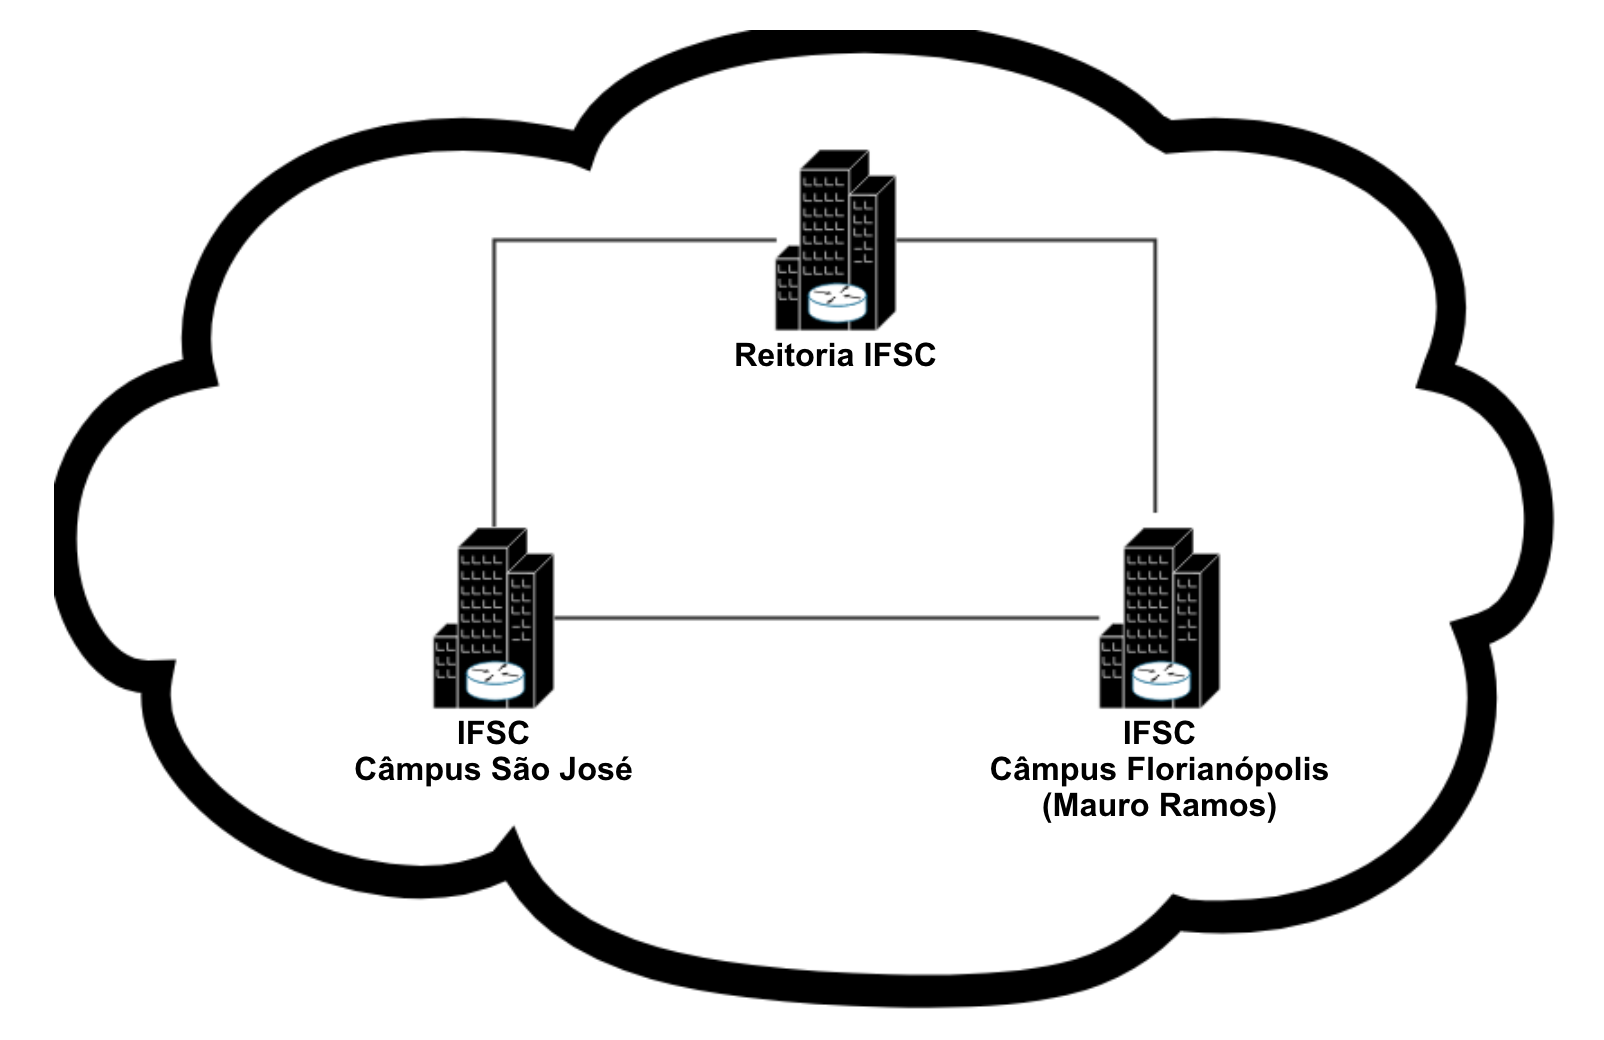
\includegraphics[width=14cm]{TCC/figuras/4-proposta/IFSC-Cloud}
    
% 	Fonte: Elaborado pelo autor.
%  	\label{ifsc_cloud}
% \end{figure}

% Do ponto de vista de armazenamento de dados, os dados da instituição estarão armazenados em múltiplas regiões (isto é, em câmpus distintos), aumentando a replicação destas informações e diminuindo assim o risco de perda de informações devido a pontos únicos de falha no sistema. Isto pode ser exemplificado, por exemplo, por um desastre de interrupção \textbf{local} do serviço em um dos câmpus da instituição. Mesmo que os dados armazenados no câmpus sejam perdidos os mesmos estarão disponíveis em outros câmpus. O sistema de armazenamento sugerido neste trabalho, Ceph, permite que \textit{backups} de dados sejam realizados de diversas formas. Dentre estas formas destacam-se a replicação de dados para outro \textit{cluster} Ceph (\textit{Ceph-on-Ceph}) e \textit{snapshots} geradas pelo sistema de armazenamento \cite{cephbackup}. Além disso, o Rook, plataforma de armazenamento que automatiza a utilização do Ceph em \textit{clusters} Kubernetes, também possibilita outras alternativas de \textit{backup}, como cópia dos dados armazenados nos volumes utilizados por contêineres, por exemplo.

% A descentralização da infraestrutura aumenta também a tolerância a falha dos serviços, pois, como explicado, os serviços fornecidos pela instituição também estarão disponíveis em múltiplas regiões, diminuindo assim a probabilidade destes ficarem indisponíveis devido a incidentes regionais em cada câmpus, como panes elétricas ou instabilidade nos enlaces de conexão da instituição, por exemplo.

% A expansão da infraestrutura de serviços para outros câmpus facilitará também a transição do modelo de gestão de serviços e \ac{TI} no \ac{IFSC} para um modelo mais descentralizado e colaborativo. Isto significa que funcionários de outros câmpus também poderão participar da manutenção e gestão efetiva dos serviços e infraestrutura da instituição. Este modelo de gestão descentralizada permitirá que não apenas mais pessoas participem na manutenção do sistema, mas também que funcionários que possuam interesse em trabalhar com a gestão deste sistema tenham esta oportunidade. Esta é, portanto, uma proposta que envolve não apenas a reestruturação da infraestrutura de serviços da instituição, mas também uma proposta de remodelagem de gestão de \ac{TI} no \ac{IFSC}.

% A implantação desta infraestrutura descentralizada poderá ocasionar a necessidade de adoção de outras tecnologias que garantam o funcionamento do sistema de forma eficiente. A utilização de \ac{QoS} na rede federada ou estabelecimento de \textit{caches} para armazenamento de dados frequentemente acessados em outros câmpus são exemplos de tecnologias que devem ser levadas em consideração. Entretanto, tais necessidades poderão ser apenas confirmadas e/ou efetivamente consideradas na implantação do sistema e em testes para verificação de seu desempenho.

% % Considerando a capacidade de processamento atual da instituição, tendências tecnológicas e \textit{hardware} legado e atual, propõe-se que a infraestrutura de serviços da instituição consista em uma nuvem de contêineres. Contêineres podem ser gerenciados através de um orquestrador de contêineres, como o Kubernetes, por exemplo. Um orquestrador de contêineres permite a rápida implantação e gestão de serviços. A implantação de novos serviços através de contêineres é facilitada pois os próprios contêineres já possuem grande parte dos conteúdos (bibliotecas e códigos) necessários para sua execução, sem precisar que todo o ambiente seja configurado especificamente para sua execução. O orquestrador também facilita a manutenção dos serviços, haja vista que regras de reinicialização de contêineres, escalabilidade e tratamento de erros podem ser facilmente configurados. Contêineres são amplamente utilizados por empresas para prover serviços internos ou externos.   

% Contêineres são uma ótima alternativa para prover serviços. Entretanto, antes de discutir a implementação de serviços em uma nuvem, é necessário que se defina como os dados e informações desta nuvem serão armazenados. Isto ocorre pois estes serviços estarão armazenando dados, e esta camada inferior deve ser primeiro definida e estudada para que seja então possível a implantação dos serviços. No contexto do \ac{IFSC} propõe-se a hiperconvergência de infraestrutura, ou seja, propõe-se que tanto que processamento e armazenamento sejam realizados na mesma infraestrutura de contêineres. Mais detalhes sobre esta proposta estão descritas a seguir.


% % ----------------------------------------------------------------------- %
% \section{Sistema de armazenamento distribuído}

% Sistemas de armazenamento são utilizados para armazenar desde arquivos pessoais até bases de dados, páginas \textit{Web} e credenciais de acesso. O sistema de armazenamento utilizado determina como será o acesso aos dados armazenados em disco, possibilitando assim que a aplicação em execução não seja responsável por armazenar diretamente o arquivo em disco, os quais são gerenciados pelo sistema de arquivos.

% No contexto da infraestrutura de serviços proposta para o \ac{IFSC}, sistemas de armazenamento distribuídos também possuem um papel central na concepção do sistema. Isto ocorre por dois motivos principais, sendo o primeiro a limitação de recursos computacionais disponíveis e o segundo a utilização de uma nuvem de contêineres. O primeiro motivo é simples: diferentemente de grandes \textit{data centers}, o \ac{IFSC} possui uma baixa capacidade de escalabilidade a curto prazo devido a pequena margem de folga dos recursos computacionais disponíveis, tornando difícil a utilização de parte destes recursos exclusivamente para armazenamento. Isto significa que, caso o armazenamento e processamento fossem realizados separadamente, seria necessário realizar a divisão de \textit{hardware} entre armazenamento e processamento, o que poderia deixar uma destas áreas deficitária. Já o segundo motivo, que é a utilização de contêineres, destaca-se como uma alternativa que permite que ambos, armazenamento e processamento, sejam realizados no mesmo \textit{hardware}, mas logicamente separados. Esta abordagem é emergente e estudos e projetos têm sido desenvolvidos para tornar a implementação de sistemas de armazenamento distribuídos viável neste contexto, sendo o termo hiperconvergência utilizado para caracterizar a oferta de armazenamento e processamento em \textit{hardware} comum e logicamente separado por \textit{software} \cite{vmwarehyperconvergence}.

% Um sistema de armazenamento distribuído amplamente utilizado é o Ceph. Exemplos de organizações que utilizam o Ceph são: \textit{Western Digital}, \ac{CERN}, Cisco e \textit{Digital Ocean} \cite{cephusers}. Este sistema de armazenamento permite o armazenamento de dados através de objetos, arquivos e blocos. O Ceph é um sistema de armazenamento distribuído altamente flexível, redundante, eficiente e configurável. Ele é, entretanto, complexo tanto em sua implantação quanto manutenção. Há ferramentas que automatizam a utilização do Ceph. Entre estas ferramentas, destaca-se o Rook, uma plataforma de armazenamento para Kubernetes, ou seja, uma plataforma que pode ser utilizada na nuvem de contêineres proposta para o \ac{IFSC}. O Rook é um projeto de código livre iniciado em 2016 e que está atualmente na incubadora da \ac{CNCF} \cite{rookhistory}.

% Apesar de ainda estar em desenvolvimento durante o decorrer deste trabalho, o Rook provou ser uma solução de armazenamento que pode ser utilizada no \ac{IFSC}. Ao automatizar a implementação do Ceph esta plataforma de armazenamento permite tanto o armazenamento de dados persistentes (como bancos de dados) e de arquivos com baixa taxa de atualização (como páginas \textit{Web} e imagens, por exemplo). Esta automatização possibilita a implantação do Ceph em \textit{clusters} de contêineres e permite que a replicação, redundância e outras funcionalidades do Ceph sejam todas configuradas e aplicadas de maneira fácil e transparente no \textit{cluster}.

% O próximo capítulo mostrará a implementação do Rook em um \textit{cluster} Kubernetes para provisionamento de arquivos através de blocos de armazenamento e objetos. Os blocos de armazenamento são utilizados para armazenamento de dados persistentes dos contêineres, enquanto o armazenamento de objetos é utilizado para prover arquivos estáticos (neste caso, imagens). Esta implementação foi realizada na \ac{GCP} devido à falta de \textit{hardware} disponível no câmpus para utilização no trabalho. Para manter a implementação o mais fiel possível a um cenário real foram utilizadas máquinas virtuais ao invés da \ac{API} de gerenciamento de \textit{clusters} Kubernetes disponível na plataforma da Google. Foram utilizadas apenas três máquinas virtuais para validação do modelo, que também pode ser reproduzido em um cenário de maior escala. Detalhes da criação da infraestrutura remota, implementação do \textit{cluster} Kubernetes e provisionamento de arquivos estão detalhados no capítulo a seguir.
% ----------------------------------------------------------------------- %
% Arquivo: 5-implementacao.tex
% ----------------------------------------------------------------------- %

\chapter{Implementação do Sistema de Armazenamento Distribuído}
\label{c_implementacao}

A proposta de implementação deste trabalho consiste na criação de um \textit{cluster} Kubernetes e implantação de armazenamento distribuído utilizando a plataforma de armazenamento Rook.

O \textit{cluster} Kubernetes foi criado através da utilização de três máquinas virtuais e uma sub-rede configuradas na \ac{GCP}. A infraestrutura foi criada remotamente na \ac{GCP} utilizando o Terraform, que é uma aplicação para manutenção e gerenciamento de infraestruturas através de código. Escolheu-se a \ac{GCP} para implementação do trabalho devido ao número de créditos de teste disponíveis para utilização na plataforma, mas outros provedores de infraestrutura tais como \ac{AWS} ou \textit{Microsoft Azure} poderiam ter sido utilizados já que o Terraform também suporta a criação de infraestruturas nestes provedores. É importante ressaltar que foram utilizadas máquinas virtuais para que o cenário implementado pudesse ser replicado tanto em outros provedores quanto localmente, não tornando assim a implementação dependente de \ac{API}s ou serviços específicos do provedor, tais como \ac{AKS} ou \ac{Amazon EKS}.

Já o \textit{cluster} Kubernetes foi criado através do Rancher, que é uma ferramenta para gerenciamento de \textit{clusters} Kubernetes. Esta ferramenta permite, por exemplo, a criação automatizada de \textit{clusters} e adição e remoção de nós de processamento ao \textit{cluster}, além de fornecer ferramentas para monitoramento dos serviços implantados. O Rancher já é utilizado no ambiente de produção da infraestrutura de serviços mantida no câmpus do \ac{IFSC} de São José.

Após a criação da infraestrutura necessária e implantação do \textit{cluster} Kubernetes, o Rook foi implantado para gerir o armazenamento do \textit{cluster}, e uma base de dados MySQL e um \textit{blog} WordPress foram instalados para utilização do armazenamento fornecido pelo Rook. Instruções detalhadas sobre a criação da infraestrutura remota e do \textit{cluster} Kubernetes estão disponíveis na seção de Anexos.

% ----------------------------------------------------------------------- %
\section{Criação da infraestrutura remota}

As especificações das máquinas virtuais utilizadas, tais como tipo de máquina utilizada e distribuição Linux instalada estão disponíveis na tabela \autoref{tabela-vms}.
\newline

\begin{table}[htb]
\centering
\caption{Especificação das máquinas virtuais}%
\label{tabela-vms}
\begin{tabular}{ccc}
\toprule
  Especificação & Valor \\
\midrule \midrule
  Tipo de máquina virtual & \textit{n1-standard-2} \\
\midrule
  Número de máquinas virtuais criadas & 3 \\
\midrule 
  Número de \textit{cores} & 2 \ac{vCPUs} \\
\midrule 
  Quantidade de memória RAM & 7.5 GB \\
\midrule
  Tipo de disco rígido & \textit{Standard persistent disk} \\
\midrule
  Quantidade de armazenamento & 15 GB \\
\midrule
  Zona e Região & \textit{southamerica-east1-a} \\
\midrule
  Distribuição Linux & Debian 9 (\textit{Stretch}) \\
\bottomrule
\end{tabular}%
{%
  \fonte{Elaborado pelo autor.}%
}
\end{table}

A sub-rede criada possui regras de \textit{firewall} específicas para permitir que apenas as portas necessárias para funcionamento dos serviços implantados e gerenciamento do \textit{cluster} Kubernetes estejam abertas. A tabela \autoref{tabela-sub-rede} mostra quais portas foram abertas para os protocolos \ac{TCP} e \ac{UDP}.

\begin{table}[htb]
\centering
\caption{Especificação da sub-rede}%
\label{tabela-sub-rede}
\begin{tabular}{ccc}
\toprule
  Especificação & Valor \\
\midrule \midrule
  Faixa de \ac{IP}s & 10.0.0.0/24 \\
\midrule 
  Tipo de endereço & Interno \\
\midrule 
  Portas de \textit{firewall} abertas para protocolo \ac{TCP} & 22, 53, 80, 443, 2380, 2379, 3306, \\
  & 6443, 6970, 6800-7300, 8124, 9283, \\
  & 10250, 10254, 30000-32767, 44134 \\
\midrule
  Portas de \textit{firewall} abertas para protocolo \ac{UDP} & 53, 8472 \\
\bottomrule
\end{tabular}%
{%
  \fonte{Elaborado pelo autor.}%
}
\end{table}

A criação da infraestrutura remota foi realizada utilizando o Terraform, que permite que componentes da infraestrutura sejam descritos como código e gerenciados através do \textit{software}. O \autoref{l_terraform-vm} mostra um trecho do código utilizado para criação de uma das máquinas virtuais utilizadas no projeto através do Terraform.

\begin{lstlisting}[language=Caml,caption=Configuração de máquina virtual descrita no arquivo de configuração do Terraform,captionpos=t,label=l_terraform-vm, numbers=none]
resource "google_compute_instance" "vm-0" {
  name         = "vm-0"
  machine_type = "n1-standard-2"
  zone         = "southamerica-east1-a"

  boot_disk {
    initialize_params {
      image = "debian-cloud/debian-9"
      size = "15"
    }
  }

  network_interface {
    subnetwork    = "${google_compute_subnetwork.subnet-0.name}"
    address       = "${google_compute_address.address-0.address}"
    access_config = {}
  }

  metadata {
    sshKeys = "${var.gce_ssh_user}:${file(var.gce_ssh_pub_key_file)}"
  }

  metadata_startup_script = "${data.template_file.startup_script.rendered}"

  tags = ["k8s"]
}
\end{lstlisting}

A sintaxe da configuração é: o recurso criado é do tipo \texttt{google\_compute\_instance} (máquina virtual) e nomeado como \texttt{vm-0}. A máquina virtual é do tipo predefinido \texttt{n1-standard-2} e localizada na zona e região \texttt{southamerica-east1-a} (São Paulo). O disco de inicialização da máquina terá armazenamento de \texttt{15 GB} e será instalada a imagem da distribuição linux \texttt{debian-cloud/debian-9}. O nome da rede ao qual a máquina será associada está definido no parâmetro \texttt{google\_compute\_subnetwork.subnet-0.name} e endereço de rede interno será o definido no parâmetro \texttt{google\_compute\_address.address-0.address}. O nome do usuário criado na máquina virtual será o armazenado na variável \texttt{var.gce\_ssh\_user} e suas chaves para acesso através \ac{SSH} estão disponíveis no arquivo referenciado pela variável \texttt{var.gce\_ssh\_pub\_key\_file}. Também será adicionado um \texttt{script} de inicialização a ser executado toda vez que a máquina for iniciada, o qual está definido em \texttt{data.template\_file.startup\_script.rendered}. Este \textit{script} está disponível no \autoref{l_startupscript_file}. Também será adicionada à máquina virtual uma \textit{tag} de valor \texttt{k8s}. O arquivo completo utilizado para criação de toda a infraestrutura está disponível no \autoref{l_terraform_file}.

Após a descrição dos componentes da infraestrutura necessários no formato aceito pelo Terraform a infraestrutura remota foi criada na \ac{GCP}. A \autoref{gcp_vms} mostra as máquinas virtuais criadas através do Terraform na \ac{GCP}.

\begin{figure}[!htpb]
	\centering
	\caption{Máquinas virtuais criadas na \ac{GCP}}
    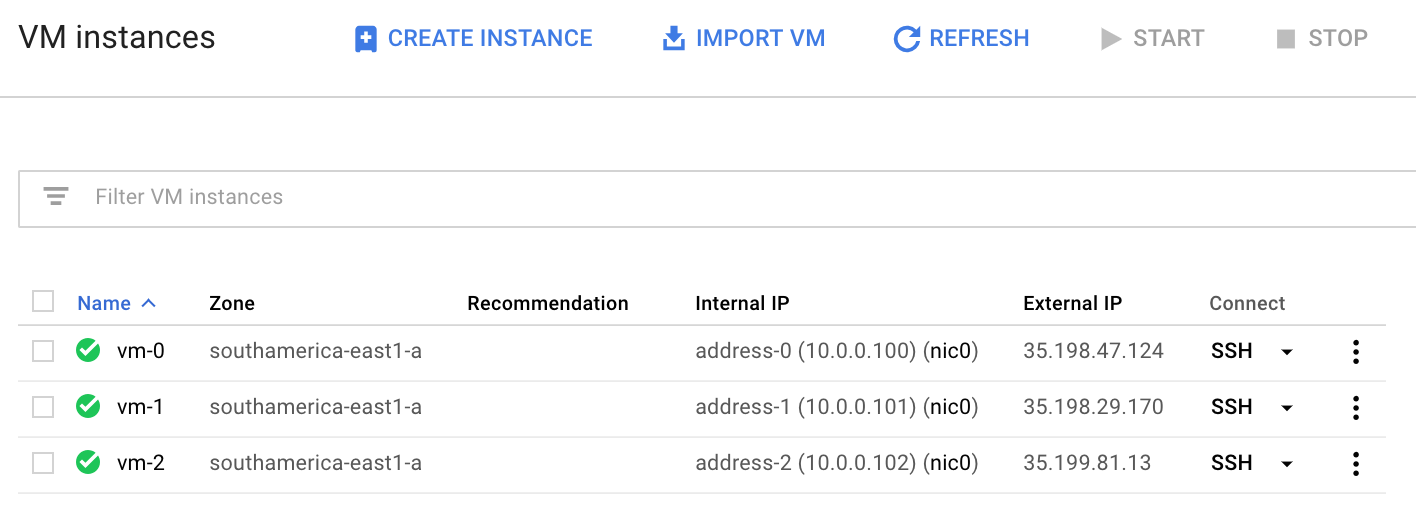
\includegraphics[width=16cm]{TCC/figuras/5-implementacao/vms}
    
	Fonte: Elaborado pelo autor.
 	\label{gcp_vms}
\end{figure}

% ----------------------------------------------------------------------- %
\section{Criação do \textit{cluster} Kubernetes}

Para criação do \textit{cluster} Kubernetes remoto foi utilizado o Rancher, que é uma ferramenta para gerenciamento de \textit{clusters} Kubernetes. Os únicos requisitos para criação do \textit{cluster} remoto utilizando o Rancher são de que os dispositivos que farão parte do \textit{cluster} possuam versões do \texttt{Docker} instalado compatíveis com a versão do Rancher utilizada e que sejam fornecidas ao Rancher chaves \ac{SSH} de um usuário que possua privilégios de administrador. Assim, os componentes necessários, como contêineres, serão automaticamente instalados e o \textit{cluster} Kubernetes criado. Escolheu-se utilizar o Rancher por dois motivos principais, sendo o primeiro a vantajosa automatização da criação do \textit{cluster} (que pode ser complexa devido as configurações de rede) e o segundo a independência de plataforma que o Rancher oferece, podendo ser utilizado para gerenciar tanto um \textit{cluster} remoto hospedado em diferentes provedores de \ac{IaaS}/\ac{PaaS} ou local.

Após a instalação do docker nas máquinas virtuais (procedimento automaticamente realizado na criação das máquinas virtuais através de um \textit{script} de inicialização) é necessário dar permissão de execução do comando \texttt{docker} ao usuário na máquina virtual. Assim, as credenciais de acesso deste usuário poderão ser utilizadas pelo Rancher para criar e configurar o \textit{cluster} Kubernetes remoto através do docker instalado nas máquinas. Parte do arquivo de configuração do Rancher utilizado nesta etapa é mostrado no \autoref{l_rancher_master}, enquanto o arquivo completo de configuração pode ser visto no \autoref{l_rancher_file}.
\newline

\begin{lstlisting}[language=Caml,caption=Configuração de nó mestre do \textit{cluster} criado com Rancher,captionpos=t,label=l_rancher_master, numbers=none]
nodes:
- address: 35.198.47.124
  internal_address: 10.0.0.100
  user: matuzalemmuller
  ssh_key_path: keys/id_rsa
  role: [controlplane,worker,etcd]
  hostname_override: master
  labels:
    node: master
}
\end{lstlisting}

Uma breve explicação sobre cada parâmetro utilizado na configuração está disponível abaixo:

\begin{itemize}
    \item \texttt{address}: endereço \ac{IP} público da máquina virtual.
    \item \texttt{internal\_address}: endereço \ac{IP} da máquina virtual na sub-rede na qual ela se encontra.
    \item \texttt{user}: usuário que será utilizado para criação do \textit{cluster}. É necessário que este usuário possua permissões de execução do \texttt{docker} e outras permissões de administrador para que o \textit{cluster} seja criado.
    \item \texttt{ssh\_key\_path}: localização das chaves \ac{SSH} do usuário utilizado no parâmetro \texttt{user} (neste caso, \texttt{matuzalemmuller}).
    \item \texttt{role}: funções do nó no \textit{cluster}. Como este será o nó mestre ele assumirá as funções de \texttt{controlplane} (\textit{master}), \texttt{worker} (executa \textit{pods}) e \texttt{etcd} (armazena as chaves-valor (\textit{key-value}) e estado de aplicações de forma distribuída).
    \item \texttt{hostname\_override}: ignora o nome da máquina virtual e utiliza um nome específico (\texttt{master}) para se referenciar a este nó.
    \item \texttt{labels}: é adicionado um \texttt{label} de valor \texttt{master} para que \textit{pods} possam ser criados especificamente neste nó ao referenciar este \texttt{label}, por exemplo.
\end{itemize}

A \autoref{k8s_nodes} mostra o \textit{cluster} disponível após sua criação com os três nós do \textit{cluster} Kubernetes em execução. A ferramenta de linha de comando \texttt{kubectl} é utilizada para gerenciamento do \textit{cluster} Kubernetes.

\begin{figure}[!htpb]
    \centering
    \caption{Saída do terminal: Nós em execução após criação de \textit{cluster} com Rancher}
\begin{verbatim}
    matuzalem-macbook:remote-setup matuzalem$ kubectl get node
    NAME      STATUS    ROLES                      AGE       VERSION
    master    Ready     controlplane,etcd,worker   1m        v1.11.1
    worker1   Ready     etcd,worker                1m        v1.11.1
    worker2   Ready     etcd,worker                1m        v1.11.1
\end{verbatim}
	Fonte: Elaborado pelo autor.
 	\label{k8s_nodes}
\end{figure}

Após a criação do \textit{cluster} um arquivo de nome \texttt{kube\_config\_cluster.yml} será criado. Este arquivo de configuração permite que o \textit{cluster} seja acessado e gerenciado externamente.

% ----------------------------------------------------------------------- %
\section{Implantação do Rook para utilização de armazenamento}

Após a criação da infraestrutura e do \textit{cluster} Kubernetes é possível instalar o Rook para que seja realizada a gestão de armazenamento no \textit{cluster}. 

A instalação do Rook consiste em três procedimentos principais, sendo o primeiro a instalação do Rook no \textit{cluster} para criação de operadores e agentes nos nós. Isto permitirá que o Ceph seja iniciado nos nós, mas nenhum disco será mapeado ainda. Para que os discos sejam mapeados pelo Rook (e consequentemente pelo Ceph) é necessário criar o \textit{cluster} Rook. Este \textit{cluster} irá criar \textit{pods} adicionais em cada nó, que consistem em \textit{monitors} e \ac{OSD}s, além do \textit{operator} criado no nó mestre. Um \textit{operator} é, de forma simples, um recurso utilizado para permitir que sejam implantados \ac{CRD}s e ciclos de automatização de tarefas ao implantar aplicações, não sendo necessário criar estas funcionalidades ao implantar as aplicações \cite{coreosoperators}. Após a instalação do Rook e criação do \textit{cluster} para mapeamento dos discos é possível utilizar o Rook para prover armazenamento. A \autoref{rook_architecture} demonstra uma arquitetura do Rook que contempla todos os tipos de armazenamento disponíveis e os componentes utilizados para prover o armazenamento.

\begin{figure}[!htpb]
	\centering
	\caption{Representação da arquitetura do Rook}
    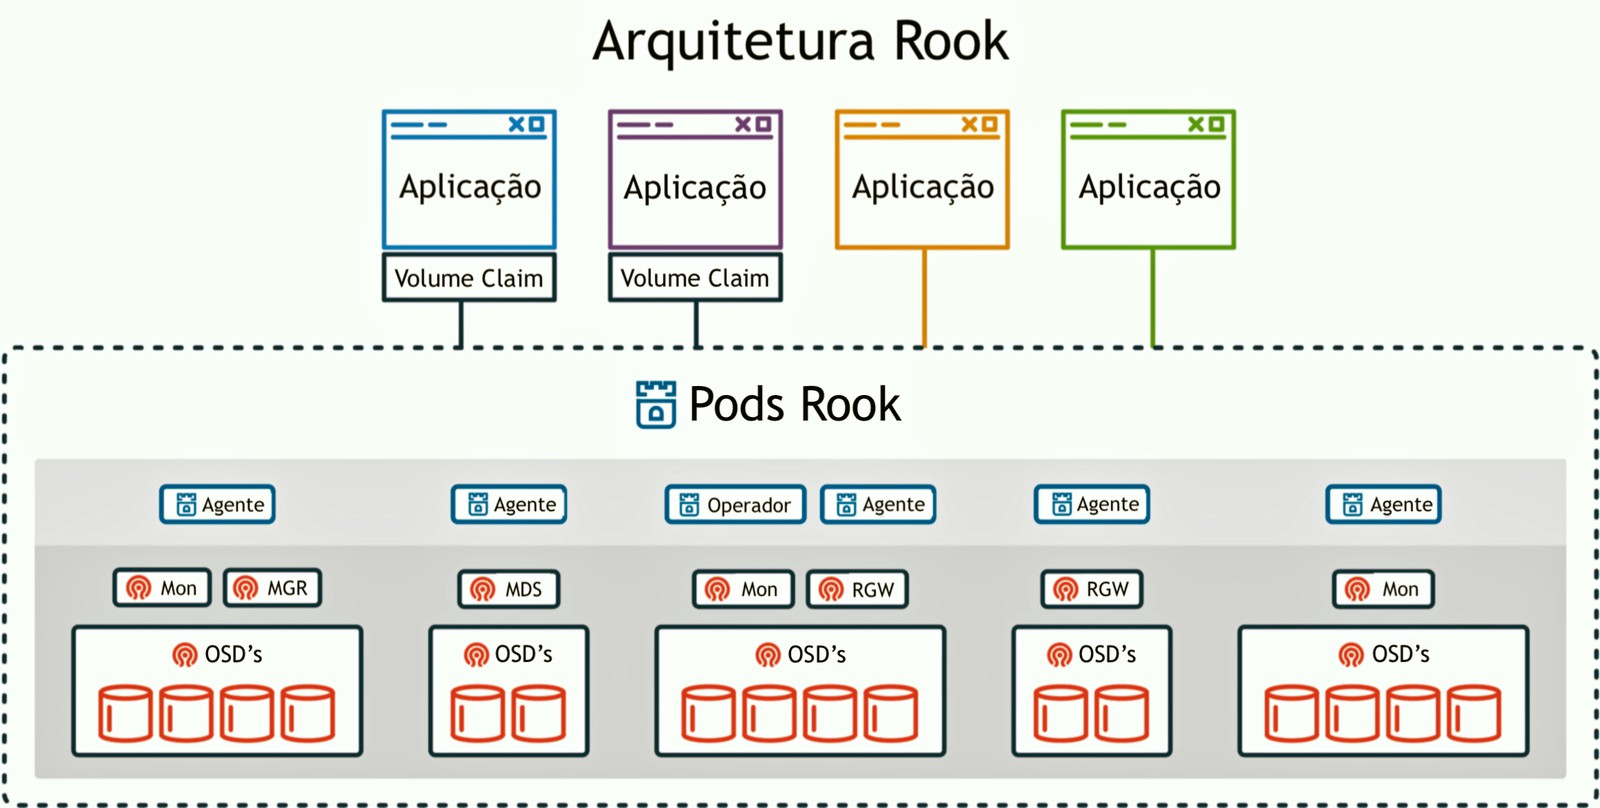
\includegraphics[width=16cm]{TCC/figuras/5-implementacao/Rook_Architecture}
    
	Fonte: Traduzido de \cite{aboutrook}.
 	\label{rook_architecture}
\end{figure}


Os componentes criados pelo Rook são diretamente equivalentes aos componentes do Ceph. Isto significa, por exemplo, que um \textit{monitor} do Rook é a implementação do \textit{monitor} do Ceph no \textit{cluster} Kubernetes. O mesmo é valido para Agentes, Operadores, \ac{OSD}s, \ac{MDS}s e \ac{RGW}s. Já as \textit{Volume Claims} representam requisições das aplicações para o \textit{cluster}, requisitando um volume para armazenamento de dados.

Em termos de implementação, o Rook \textit{operator}, que consiste nos operadores e agentes do Rook, pode ser instalado no \textit{cluster} através do Helm. Neste trabalho a versão utilizada do Rook foi a \textit{release} versão 0.8.0, a qual possui a implementação do Ceph em estado beta. Como há um mestre e dois nós no \textit{cluster} Kubernetes, serão criados no \textit{namespace} \texttt{rook-ceph-system} três \textit{pods} de \textit{agents}, um em cada nó. Além destes \textit{pods} também serão criados \textit{discovers} (responsáveis por identificar os dispositivos disponíveis para armazenamento nas máquinas virtuais) e um \textit{operator}, sendo o último disponível apenas no nó mestre. A \autoref{rook_operator_pods} mostra os componentes criados no \textit{namespace} \texttt{rook-ceph-system}.

\begin{figure}[!htpb]
	\centering
	\caption{Saída do terminal: \textit{Pods} criados pelo Rook \textit{Operator}}
    \begin{verbatim}
matuzalem-macbook:rook matuzalem$ kubectl get pod -n rook-ceph-system
NAME                                  READY     STATUS    RESTARTS   AGE
rook-ceph-agent-j7vkn                 1/1       Running   0          1m
rook-ceph-agent-lgzqm                 1/1       Running   0          1m
rook-ceph-agent-sngjz                 1/1       Running   0          1m
rook-ceph-operator-59c6b78b7c-lsz2l   1/1       Running   0          1m
rook-discover-67t94                   1/1       Running   0          1m
rook-discover-b69j4                   1/1       Running   0          1m
rook-discover-ljzqv                   1/1       Running   0          1m
    \end{verbatim}
	Fonte: Elaborado pelo autor.
 	\label{rook_operator_pods}
\end{figure}

Após realizar a inicialização do Rook \textit{operator} é possível criar o \textit{cluster} Rook. A criação do \textit{cluster} foi manualmente realizada utilizando o código disponível no \autoref{l_rook-cluster_file}. Este código cria o \textit{cluster}, \textit{namespace} e outros componentes necessários para a utilização do Rook. Neste caso os principais componentes criados serão um \textit{pod} \textit{manager}, três \textit{pods} de \textit{monitors} e três \textit{pods} de \ac{OSD}s, os quais são criados no \textit{namespace} \texttt{rook-ceph}. A \autoref{rook_cluster_pods} mostra os pods criados em execução no \textit{cluster} Rook.

\begin{figure}[!htpb]
	\centering
	\caption{Saída do terminal: \textit{Pods} criados pelo \textit{Cluster} Rook}
    \begin{verbatim}
matuzalem-macbook:rook matuzalem$ kubectl get pod -n rook-ceph
NAME                                  READY     STATUS      RESTARTS   AGE
rook-ceph-mgr-a-7944d8d79b-sjfxw      1/1       Running     0          3m
rook-ceph-mon0-5qj7l                  1/1       Running     0          4m
rook-ceph-mon1-rfvpj                  1/1       Running     0          4m
rook-ceph-mon2-xc966                  1/1       Running     0          4m
rook-ceph-osd-id-0-6cdfc557f-n6hdk    1/1       Running     0          3m
rook-ceph-osd-id-1-5475fbb74-wbh74    1/1       Running     0          3m
rook-ceph-osd-id-2-5f68f97d4d-87hpx   1/1       Running     0          3m
rook-ceph-osd-prepare-master-7dbhx    0/1       Completed   0          3m
rook-ceph-osd-prepare-worker1-cwzf7   0/1       Completed   0          3m
rook-ceph-osd-prepare-worker2-cqbc2   0/1       Completed   0          3m
    \end{verbatim}
	Fonte: Elaborado pelo autor.
 	\label{rook_cluster_pods}
\end{figure}

Agora que o \textit{cluster} Rook foi criado é possível configurá-lo para utilizá-lo para prover o armazenamento de objetos, blocos ou arquivos. Neste trabalho os tipos de armazenamento utilizados serão blocos e objetos.

O armazenamento em blocos será utilizado para gestão de volumes persistentes a serem utilizados por contêineres, os quais persistem dados após seu reinício. Isto permite, por exemplo, que os contêineres não percam suas configurações ou estados. Esta é uma boa forma de armazenar configurações e conteúdos que são frequentemente modificados por contêineres. Já o armazenamento através de objetos será utilizado para armazenar e distribuir conteúdos estáticos, tais como imagens e arquivos que são pouco modificados.

O armazenamento em blocos pode ser implementado no Rook através de um \textit{StorageClass}, enquanto o armazenamento de objetos é disponibilizado através de uma \textit{Object Store}. Ambos serão explicados nos parágrafos seguintes.

Para a configuração do armazenamento de dados através de objetos é necessário criar um \textit{StorageClass} específico do Rook. A criação deste \textit{StorageClass} é realizado utilizando o código disponível no \autoref{l_rook-storage-class_file}. Após a criação deste \textit{StorageClass} volumes persistentes (\ac{PV}) poderão ser criados através de requisições de volumes (\ac{PVC}) ao Rook.

Já para o armazenamento de objetos no \textit{cluster} Rook é necessário que uma \textit{Object Store} seja criada. Uma \textit{Object Store} é um \ac{CRD} criado pelo Rook e possui como função criar os componentes necessários para gerenciamento dos objetos no \ac{RADOS} do Ceph, fornecendo assim acesso a estes objetos através de um \textit{pod} equivalente ao \ac{RADOS} \textit{Gateway}. Assim como o \ac{RADOS} \textit{Gateway} oferece uma \ac{REST} \ac{API} de acesso compatível com a interface S3 da Amazon aos objetos armazenados, o \textit{cluster} Rook também permite que arquivos sejam gerenciados através desta \ac{API}. Logo, é possível criar \textit{buckets} no \textit{cluster} Rook, os quais serão utilizados para armazenar dados estáticos e publicamente acessíveis. Neste trabalho um domínio \texttt{.cc} foi utilizado para validação do modelo, utilizando assim o balanceamento de carga de requisições \ac{HTTP} também através de \ac{DNS}.

A \autoref{rook_rgw_pod} mostra o \textit{pod} criado para execução do \ac{RADOS} \textit{gateway} no \textit{cluster} Rook, juntamente com os outros \textit{pods} disponíveis no namespace \texttt{rook-ceph}.

\begin{figure}[!htpb]
	\centering
	\caption{Saída do terminal: \textit{Pod} \ac{RADOS} \textit{Gateway} em execução}
    \begin{verbatim}
matuzalem-macbook:rook matuzalem$ kubectl get pod -n rook-ceph
NAME                                     READY   STATUS     RESTARTS  AGE
rook-ceph-mgr-a-7944d8d79b-sjfxw         1/1     Running    0         10m
rook-ceph-mon0-5qj7l                     1/1     Running    0         11m
rook-ceph-mon1-rfvpj                     1/1     Running    0         11m
rook-ceph-mon2-xc966                     1/1     Running    0         10m
rook-ceph-osd-id-0-6cdfc557f-n6hdk       1/1     Running    0         10m
rook-ceph-osd-id-1-5475fbb74-wbh74       1/1     Running    0         10m
rook-ceph-osd-id-2-5f68f97d4d-87hpx      1/1     Running    0         10m
rook-ceph-osd-prepare-master-7dbhx       0/1     Completed  0         10m
rook-ceph-osd-prepare-worker1-cwzf7      0/1     Completed  0         10m
rook-ceph-osd-prepare-worker2-cqbc2      0/1     Completed  0         10m
rook-ceph-rgw-my-store-fdd764948-vb7fx   1/1     Running    0         13s
    \end{verbatim}
	Fonte: Elaborado pelo autor.
 	\label{rook_rgw_pod}
\end{figure}

% ----------------------------------------------------------------------- %
\section{Implantação de serviços para utilizar armazenamento}

Para utilização do armazenamento foram implantados uma base dados MySQL e um \textit{blog} WordPress. A base de dados é necessária para o funcionamento do \textit{blog} WordPress. A base de dados MySQL utiliza armazenamento em blocos na forma de volumes, enquanto o \textit{blog} WordPress utiliza armazenamento tanto na forma de objetos quanto em blocos. A seguir serão descritas as implementações destes serviços na nuvem remota.

\subsection{MySQL}

A implementação da base de dados MySQL foi realizada através da instalação do serviço pelo Helm. Como é utilizado um gerenciador de pacotes para realizar a instalação da base de dados a sua implantação é rápida e automatizada.

Para utilização do armazenamento em blocos o \textit{pod} MySQL realiza uma \ac{PVC} ao Rook, ou seja, o \textit{pod} solicita a criação de um volume de dados persistentes (\ac{PV}) ao Rook para que este volume seja utilizado como um bloco de armazenamento. O Rook, por sua vez, fornece ao \textit{pod} MySQL o volume requisitado. A \autoref{mysql_pvc_pv} mostra a requisição do volume (\ac{PVC}) realizada pelo \textit{pod} MySQL e o volume (\ac{PV}) entrege ao \textit{pod} pelo Rook.

\begin{figure}[!htpb]
	\centering
	\caption{Saída parcial do terminal: Requisição de volume e volume utilizado pelo \textit{pod} MySQL}
    \begin{verbatim}
matuzalem-macbook:tcc-engtelecom matuzalem$ kubectl get pvc
NAME      STATUS    VOLUME                                    CAPACITY
mysql     Bound     pvc-c3428e0b-f66b-11e8-939f-42010a000064  5Gi      
matuzalem-macbook:tcc-engtelecom matuzalem$ kubectl get pv
NAME                                      CAPACITY  STORAGECLASS
pvc-c3428e0b-f66b-11e8-939f-42010a000064  5Gi       rook-ceph-block
    \end{verbatim}
	Fonte: Elaborado pelo autor.
 	\label{mysql_pvc_pv}
\end{figure}

A \autoref{mysql_pod} mostra o \textit{pod} MySQL em execução, poucos momentos após sua criação.

\begin{figure}[!htpb]
	\centering
	\caption{Saída do terminal: \textit{Pod} MySQL em execução}
    \begin{verbatim}
matuzalem-macbook:tcc-engtelecom matuzalem$ kubectl get pod
NAME                                     READY     STATUS    RESTARTS   AGE
mysql-56655cb669-2zgvc                   1/1       Running   0          3m
    \end{verbatim}
    
	Fonte: Elaborado pelo autor.
 	\label{mysql_pod}
\end{figure}

\subsection{WordPress}

A implementação do WordPress também foi realizada através do Helm, ou seja, o serviço foi rapidamente criado no \textit{cluster} Kubernetes e o Rook foi utilizado para gerir o armazenamento utilizado pelo WordPress. Assim como no \textit{pod} MySQL, um volume também foi criado e associado ao \textit{pod} WordPress através de uma \ac{PVC}. Ambos volume e requisição são mostrados na \autoref{apps_pvc_pv}, juntamente com o volume e requisição do serviço MySQL.

\begin{figure}[!htpb]
	\centering
	\caption{Saída parcial do terminal: Requisição de volume e volume utilizado pelo \textit{pod} WordPress}
    \begin{verbatim}
matuzalem-macbook:tcc-engtelecom matuzalem$ kubectl get pvc
NAME        STATUS    VOLUME                                     CAPACITY
mysql       Bound     pvc-c3428e0b-f66b-11e8-939f-42010a000064   5Gi
wordpress   Bound     pvc-f035bafe-f66c-11e8-939f-42010a000064   5Gi
matuzalem-macbook:tcc-engtelecom matuzalem$ kubectl get pv
NAME                                       CAPACITY   STORAGECLASS
pvc-c3428e0b-f66b-11e8-939f-42010a000064   5Gi        rook-ceph-block
pvc-f035bafe-f66c-11e8-939f-42010a000064   5Gi        rook-ceph-block
    \end{verbatim}
	Fonte: Elaborado pelo autor.
 	\label{apps_pvc_pv}
\end{figure}

A \autoref{wordpress_pod} mostra que o \textit{pod} WordPress também está em execução. É possível perceber que há quatro \textit{pods} em execução no \textit{namespace} \texttt{default}: um do MySQL, outro do WordPress e dois referentes ao NGINX \textit{controller}. Os \textit{pods} do NGINX funcionam como controladores \textit{Ingress} para que o serviço WordPress possa ser acessado externamente. O NGINX pode ser instalado através do Helm e a interação entre os serviços NGINX e WordPress ocorre automaticamente, ou seja, ao instalar o WordPress ele pode ser automaticamente configurado para ser acessado através do NGINX.

\begin{figure}[!htpb]
	\centering
	\caption{Saída do terminal: \textit{Pod} WordPress em execução}
    \begin{verbatim}
matuzalem-macbook:tcc-engtelecom matuzalem$ kubectl get pod
NAME                                                  READY     STATUS   AGE
mysql-56655cb669-2zgvc                                1/1       Running  13m
nginx-nginx-ingress-controller-7dd6474678-5jkqs       1/1       Running  24m
nginx-nginx-ingress-default-backend-5b88698ddc-zc242  1/1       Running  24m
wordpress-wordpress-5fb9cdfcfd-nr7rt                  1/1       Running  5m
    \end{verbatim}
	Fonte: Elaborado pelo autor.
 	\label{wordpress_pod}
\end{figure}

A \autoref{wordpress_blog} mostra a página \textit{web} do \textit{blog} WordPress em execução.

\begin{figure}[!htpb]
	\centering
	\caption{\textit{Blog} WordPress}
    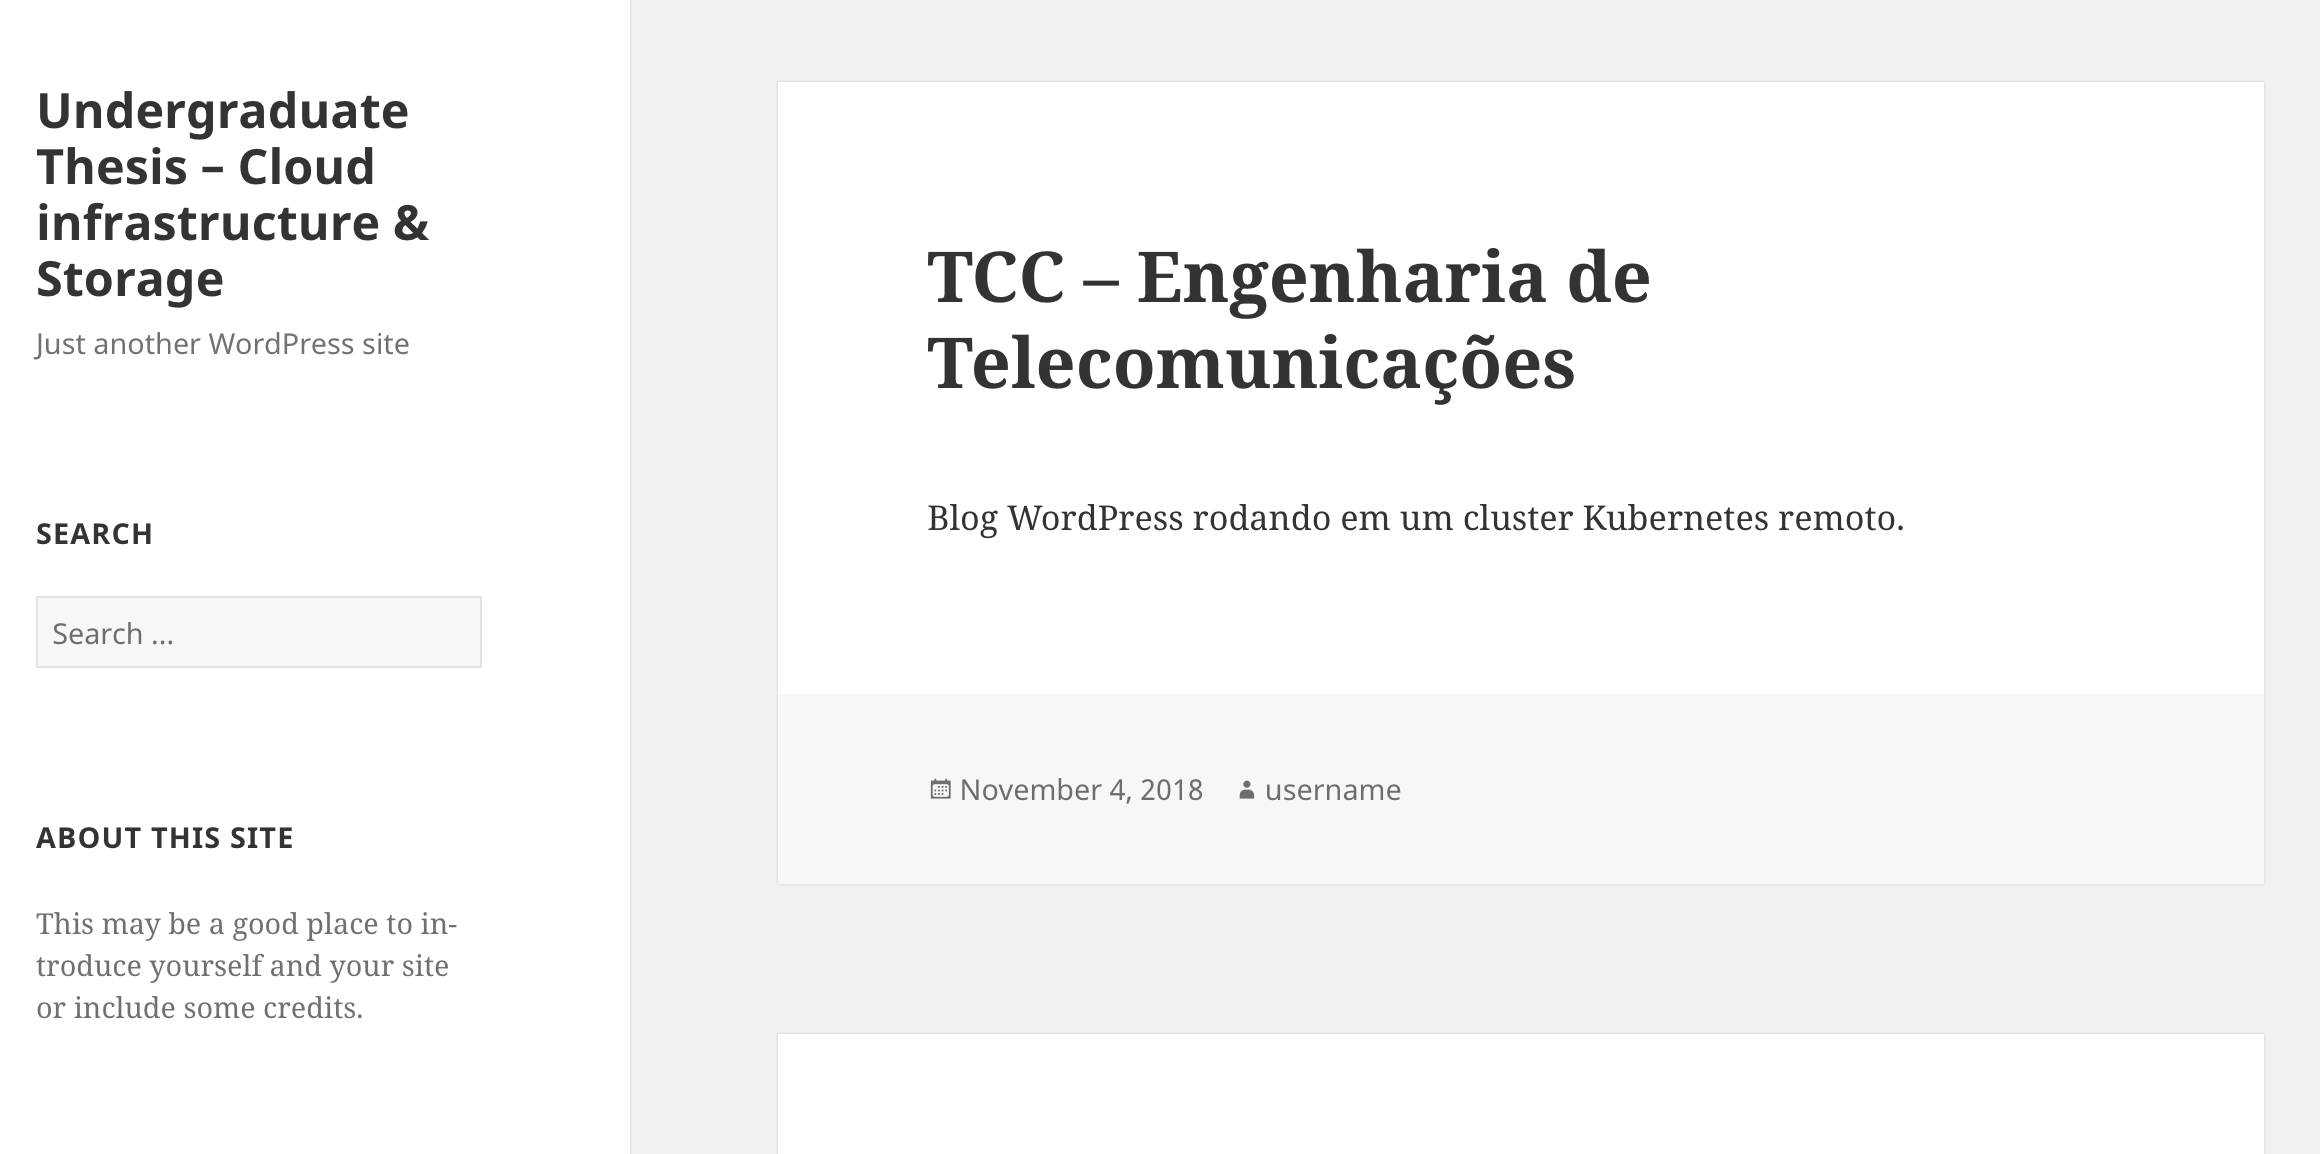
\includegraphics[width=16cm]{TCC/figuras/5-implementacao/wordpress-blog}
    
	Fonte: Elaborado pelo autor.
 	\label{wordpress_blog}
\end{figure}

Até esta etapa o Rook está sendo utilizado para prover armazenamento através de volumes requisitados pelos serviços implantados. Isto significa que o armazenamento utilizado é em blocos, e o armazenamento de objetos ainda não foi utilizado.

Para utilizar o armazenamento de objetos da forma proposta é necessário armazenar objetos na \textit{Object Store} do Rook e tornar estes objetos publicamente acessíveis. Neste trabalho uma imagem será salva como um objeto na \textit{Object Store} do Rook e ela será utilizada pelo WordPress no \textit{blog}. Para isto, é necessário criar um usuário no \ac{RADOS} \textit{gateway} e utilizar este usuário para criar um \textit{bucket} e administrar o armazenamento dos objetos. Após a criação do usuário e \textit{bucket} é possível armazenar uma imagem como objeto na \textit{Object Store}. A imagem utilizada neste projeto é a da \autoref{object_image}. Esta imagem não possui direitos autorais, é do tipo \texttt{jpg} e possui 179 KB.

\begin{figure}[!htpb]
	\centering
	\caption{Imagem armazenada como objeto}
    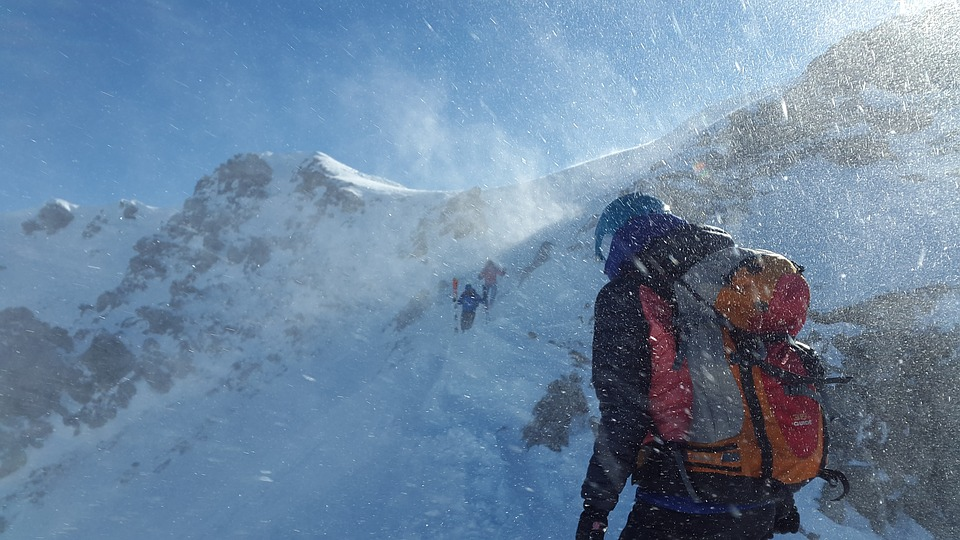
\includegraphics[width=15cm]{TCC/figuras/5-implementacao/example-image}
    
	Fonte: \cite{image}
 	\label{object_image}
\end{figure}

Agora que a imagem está armazenada como um objeto é necessário torna-lá publica, o que pode ser feito através da utilização do \textit{Ingress} NGINX. O código utilizado para implantar o recurso \textit{ingress} está disponível no \autoref{l_rook-object_ingress_file}. 

Com a imagem publicada é possível utilizá-la no WordPress. A \autoref{wordpress_post} mostra a utilização da imagem em uma publicação no WordPress.

\begin{figure}[!htpb]
	\centering
	\caption{Publicação WordPress utilizando imagem armazenada como objeto}
    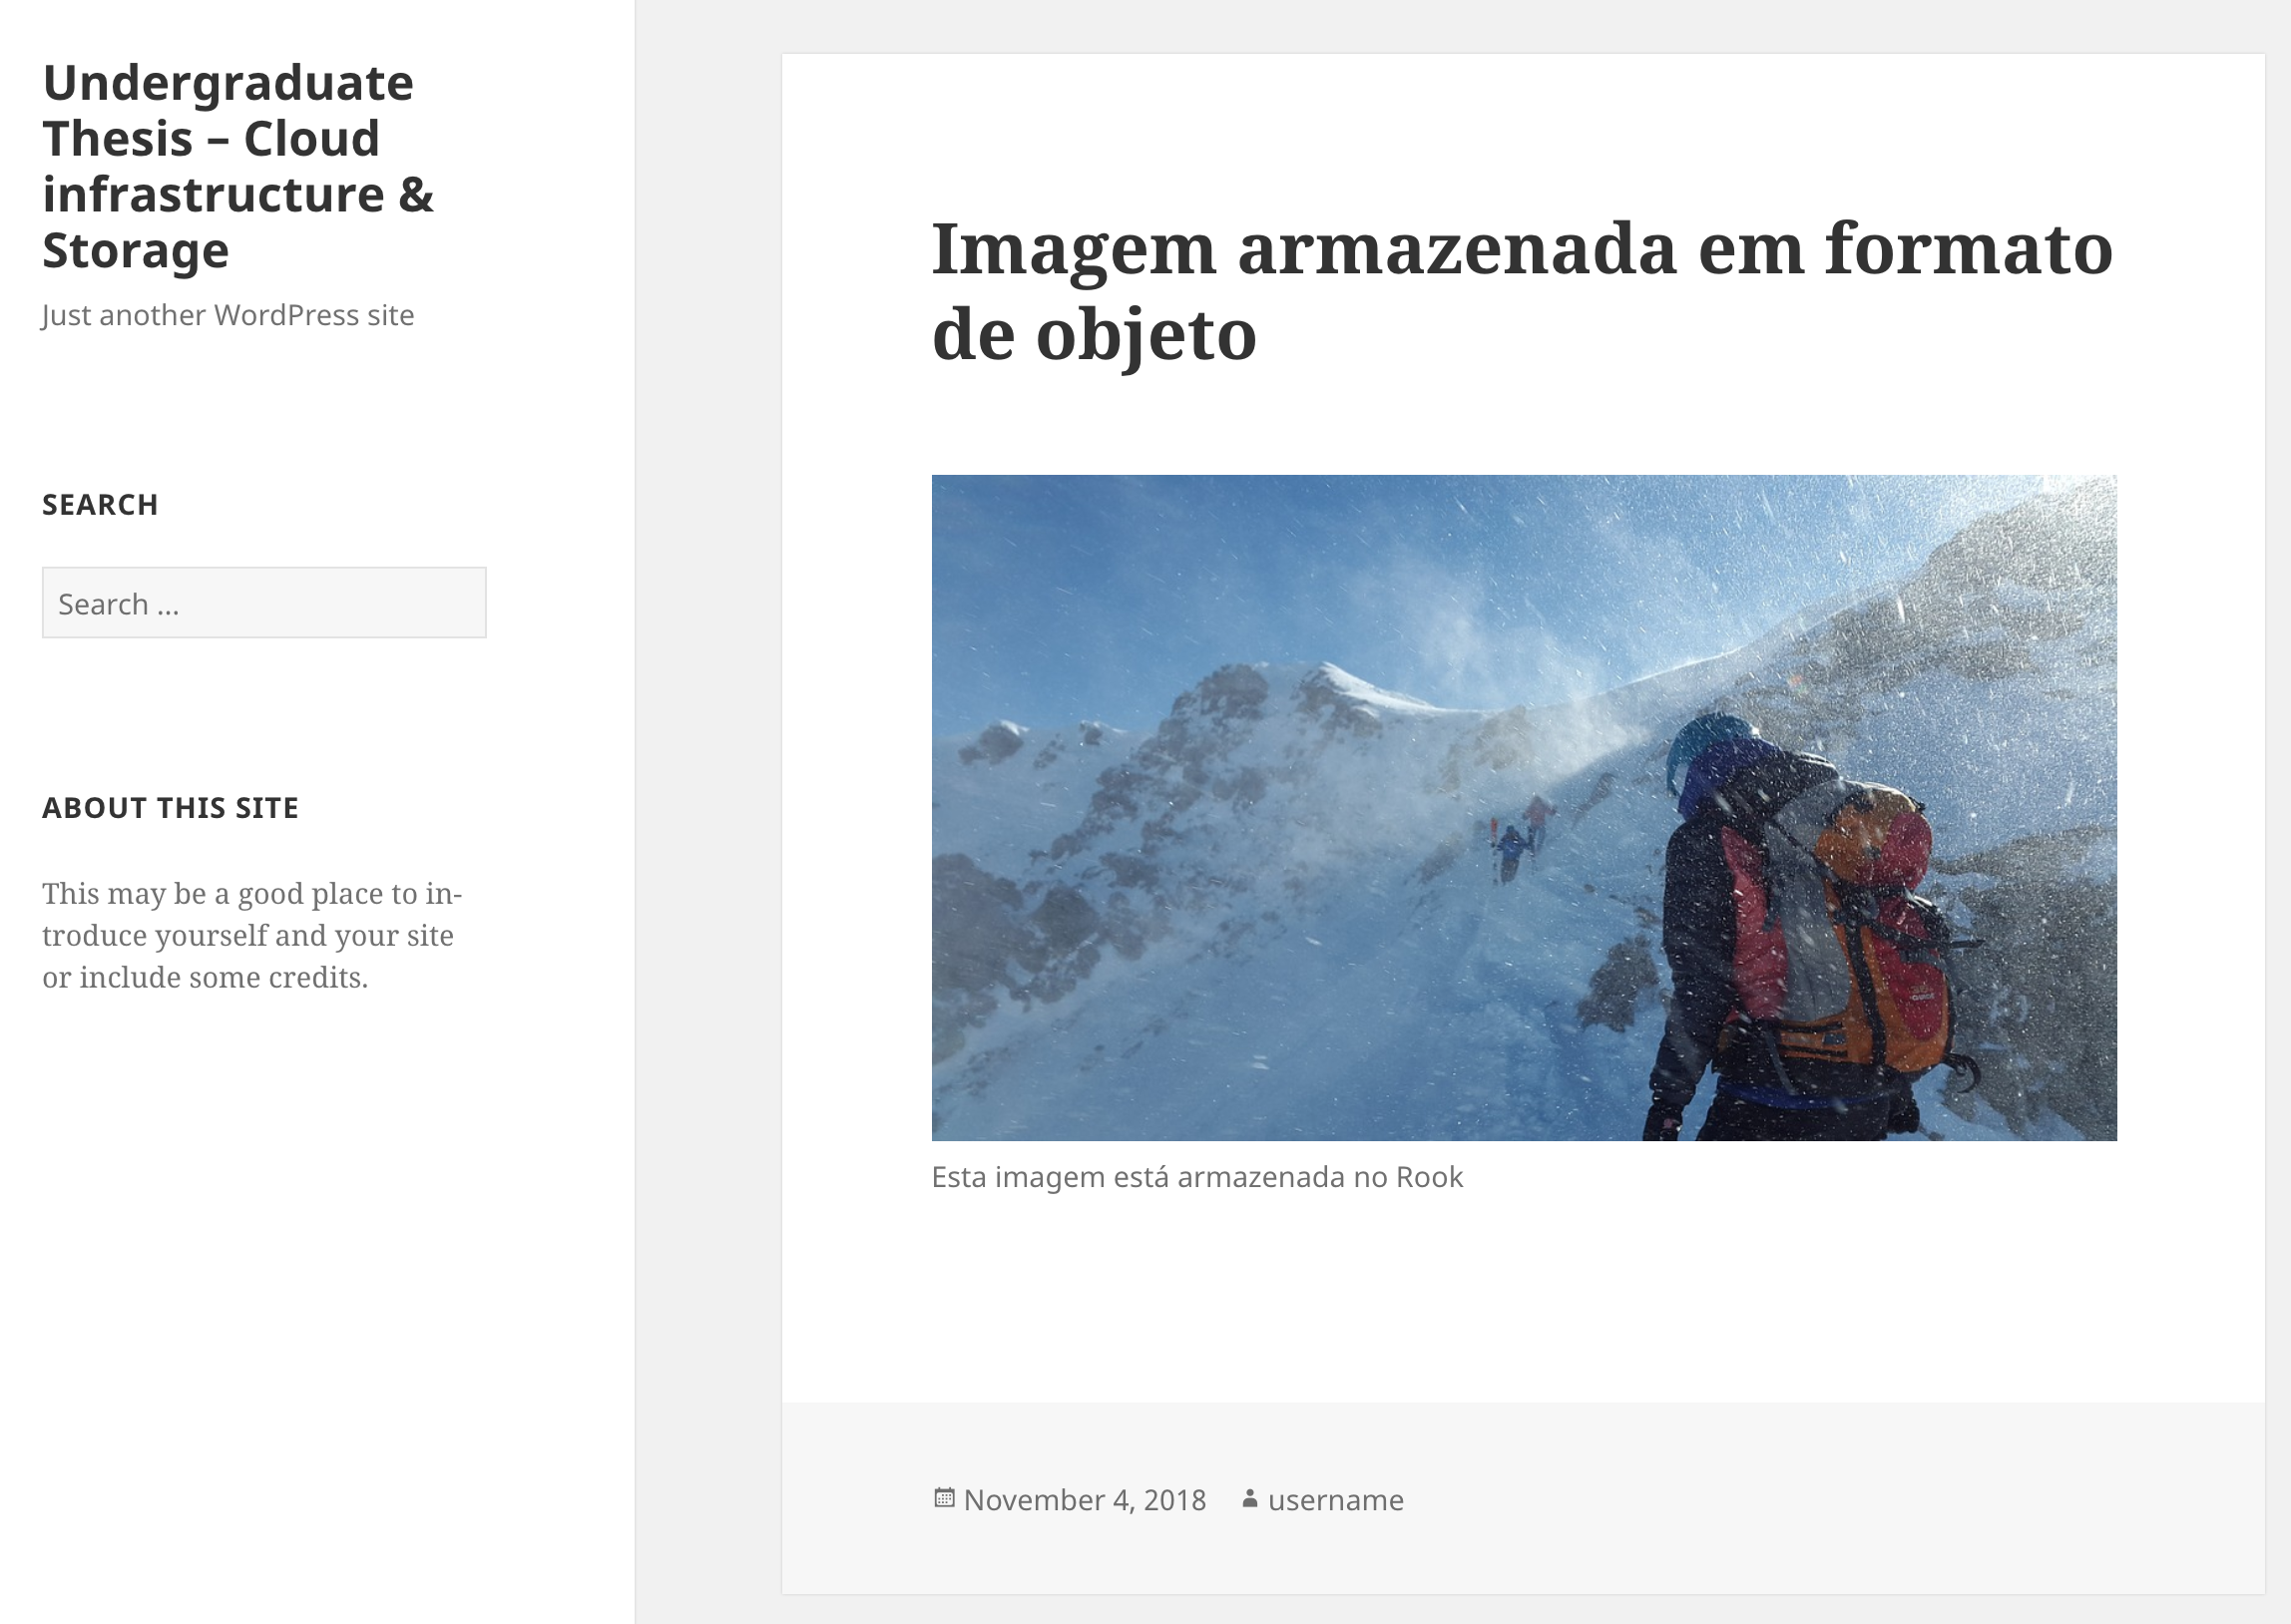
\includegraphics[width=15cm]{TCC/figuras/5-implementacao/wordpress-post}
    
	Fonte: Elaborado pelo autor.
 	\label{wordpress_post}
\end{figure}

A \autoref{wordpress_mysql_schematic} é um diagrama geral da implementação realizada neste trabalho. Os objetos \texttt{Deploment}, \texttt{ReplicaSet}, \texttt{MySQL Pod} e \texttt{WordPress Pod} são automaticamente criados através da instalação de \textit{charts} disponíveis no Helm. As \ac{PVC} são realizadas ao \texttt{StorageClass}, que cria volumes (\ac{PV}) a serem utilizados pelos \texttt{Pods}. Já o objeto \texttt{RGW} é criado através da \textit{Object Store} do Rook. É importante ressaltar que ambos o \texttt{StorageClass} e \texttt{RGW} são \ac{CRD}s do Rook e utilizam o Ceph para armazenamento dos dados. O \texttt{Ingress Controller}, por sua vez, é configurado por objetos \textit{Ingress} automaticamente criados pelas aplicações. A automatização na implantação de serviços e gerenciamento dos recursos comprova a facilidade de utilização do Kubernetes, além de sua eficácia em fornecer uma única plataforma de gerenciamento que combina rede, armazenamento e computação, caracterizando assim este modelo como uma infraestrutura hiperconvergente.

\begin{figure}[!htpb]
	\centering
	\caption{Esquemático da implementação}
    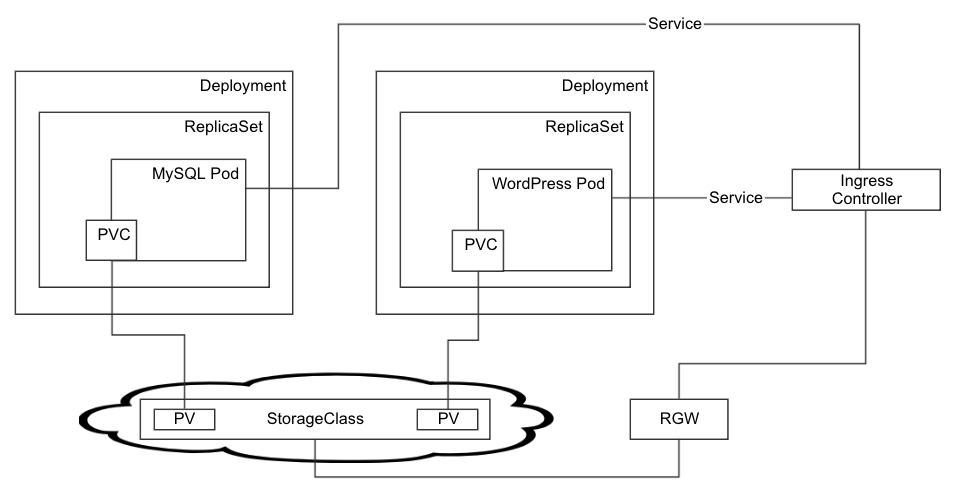
\includegraphics[height=7cm]{TCC/figuras/5-implementacao/apps-schematic.png}
    
	Fonte: Elaborado pelo autor.
 	\label{wordpress_mysql_schematic}
\end{figure}
% % ----------------------------------------------------------------------- %
% % Arquivo: 6-implantacao-no-ifsc.tex
% % ----------------------------------------------------------------------- %

% \chapter{Plano de implantação da infraestrutura de serviços proposta}
% \label{implantacao_no_ifsc}

% O capítulo anterior demonstra que a utilização do Rook - mesmo que ainda em estágio de desenvolvimento - pode satisfazer as necessidades de armazenamento persistente de serviços via blocos e objetos, podendo assim ser utilizado na infraestrutura de serviços proposta para o \ac{IFSC}.

% A implementação da infraestrutura de contêineres proposta para o \ac{IFSC} caracteriza-se como um processo contínuo de melhoria, o qual deve ser planejado a longo prazo e ter apoio de diversos setores da instituição, haja vista que é preciso que haja não apenas uma reorganização da infraestrutura da instituição, mas também uma alteração na governança de \ac{TI}.

% Como mostrado na \autoref{fluxograma_implantacao}, o plano de implantação da infraestrutura de serviços proposta para o \ac{IFSC} divide-se em quatro etapas principais: adequação das políticas de \ac{TI} do \ac{IFSC}, implementação de nuvens de contêineres locais nos câmpus da instituição, integração das nuvens locais e utilização da nova infraestrutura no ambiente de produção. Estas etapas são descritas nas subseções a seguir.

% \begin{figure}[!htpb]
% 	\centering
% 	\caption{Fluxograma de implantação da infraestrutura proposta no \ac{IFSC}}
%     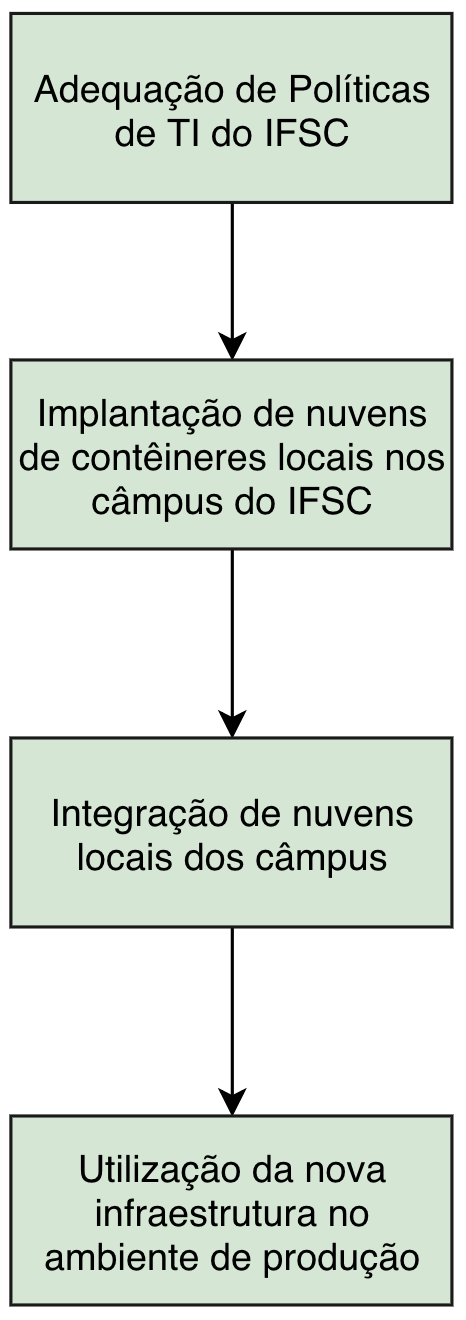
\includegraphics[height=13cm]{TCC/figuras/6-plano/Fluxograma-Plano_IFSC}
    
% 	Fonte: Elaborado pelo autor.
%  	\label{fluxograma_implantacao}
% \end{figure}

% \section{Adequação das Políticas de TI}

% A formação de funcionários para melhoria da infraestrutura dos câmpus e a melhoria das infraestruturas em si caracterizam-se como o primeiro passo do plano de implantação da infraestrutura de serviços baseadas em contêineres proposta para o \ac{IFSC}.

% Devido a descentralização da infraestrutura de serviços proposta para a instituição será necessário que haja uma alta coordenação entre os departamentos de \ac{TIC} para manutenção e expansão do sistema. É importante ressaltar que as funções destes departamentos nos câmpus do \ac{IFSC} permanecerão as mesmas, sendo que as funções dos departamentos na manutenção da infraestrutura - até o momento local e física - também permanecerão os mesmas, mas agora em um ambiente virtual e descentralizado.

% É possível observar na \autoref{organograma_ifsc} que as \ac{CTIC}s estão abaixo dos departamentos de administração dos câmpus onde elas se encontram. Isto significa que a influência da \ac{DTIC} sobre estes departamentos dá-se principalmente através das políticas de governança e do \ac{PDTI} da instituição, visto que a \ac{DTIC} não é diretamente responsável pelas \ac{CTIC}s de cada câmpus.

% \begin{figure}[!htpb]
% 	\centering
% 	\caption{Organograma simplificado dos departamentos de \ac{TIC} do \ac{IFSC}}
%     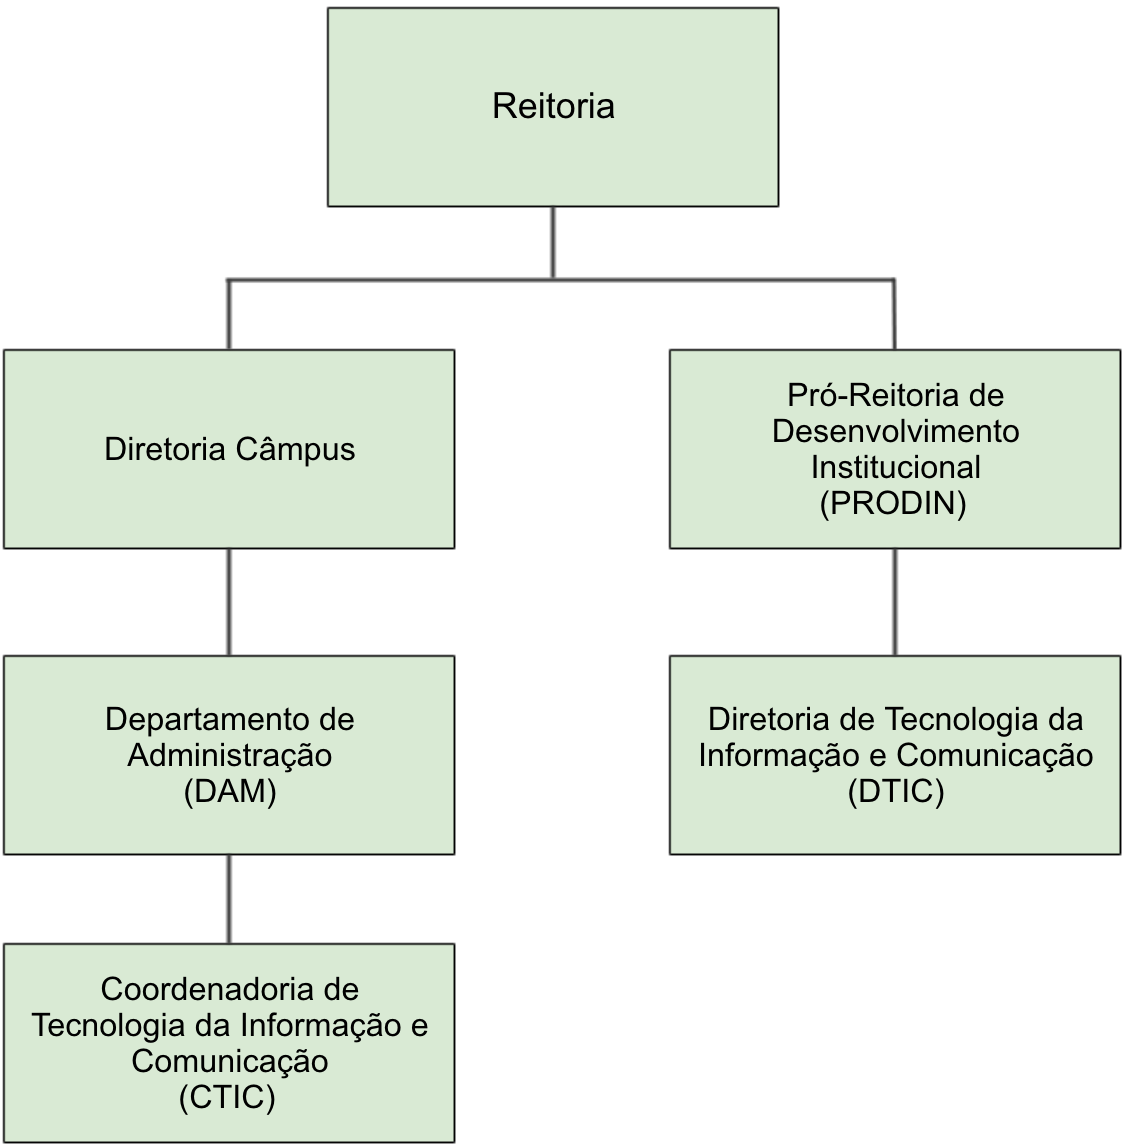
\includegraphics[width=11cm]{TCC/figuras/6-plano/Organograma-CTIC_DTIC}
    
% 	Fonte: Elaborado pelo autor.
%  	\label{organograma_ifsc}
% \end{figure}

% Propõe-se, portanto, que sejam adicionadas ao \ac{PDTI} ações que promovam a formação dos funcionários focada nas necessidades de infraestrutura dos câmpus, resultado assim no alinhamento dos serviços e infraestruturas da instituição. Na prática a convergência das infraestruturas locais facilitará a sua posterior integração e manutenção, o que é vantajoso para a instituição. 

% É importante ressaltar que o \ac{PDTI} já promove ações para formação de funcionários da instituição. De acordo com o \ac{PDTI} de 2018, por exemplo, o plano a executar em 2018 para capacitação promove diversos cursos para formação dos funcionários, tais como ``IOS SWIFT BOOTCAMP'' e ``Mobile Apps para iOS e Android com HTML5 e PhoneGap'' \cite{pdti2018}. Sugere-se que cursos nas áreas de ``Segurança de Redes e Sistemas'' e ``Administração e Projetos de Redes'' (também ofertados atualmente) tenham mais enfoque, visando melhorar as infraestruturas locais dos câmpus para melhor integração futura dos serviços. Pode-se, por exemplo, classificar as necessidades de cada câmpus da instituição e atribuir-se prioridades a cada necessidade, facilitando assim a escolha de cursos de formação e treinamento para funcionários do \ac{IFSC} baseados nestas prioridades. Caso possível, os cursos de formação nas áreas propostas podem ser ofertados por funcionários da própria instituição, economizando assim recursos que seriam gastos em cursos externos.

% \section{Implantação de nuvens de contêineres locais nos câmpus}

% O segundo passo na implantação da infraestrutura proposta é que sejam implantadas nuvens de contêineres locais em cada câmpus da instituição. Estas nuvens serão nuvens de testes, as quais possibilitarão que funcionários da instituição se familiarizem com nuvens de contêineres, além de possibilitar testes de portabilidade dos serviços atualmente ofertados pela instituição para este ambiente.

% Alguns dos serviços ofertados pela instituição podem ser facilmente implementados em nuvens de contêineres através da utilização de versões (imagens) estáveis das aplicações, como o Moodle e a plataforma de e-mail Zimbra, por exemplo. Outros serviços, como o \ac{SIG}, precisarão ser portados para a forma de contêiner. Esta etapa do planejamento caracteriza-se, portanto, como o estudo das tecnologias que serão utilizadas na infraestrutura e adequação destas tecnologias ao cenário do \ac{IFSC}.

% É importante ressaltar que a comunidade acadêmica também pode ser envolvida nesta etapa, incentivando tanto professores quanto alunos a conduzir projetos e trabalhos de conclusão de curso que colaborem com o projeto (a exemplo deste trabalho).

% \section{Integração de nuvens de contêineres locais dos câmpus}

% A terceira etapa da implantação da infraestrutura de serviços proposta é a integração das nuvens locais de cada câmpus. Isto permitirá que tenha-se um melhor entendimento das necessidades do sistema, tanto do posto de vista de administração do sistema quanto de recursos físicos necessários para a realização do projeto.

% Nesta etapa poderão ser discutidas e determinadas as funções de cada câmpus/funcionário na manutenção do sistema, delegando funções específicas para membros das equipes de \ac{TIC} que participarem diretamente na administração do sistema. Por exemplo, um membro do departamento da \ac{CTIC} do câmpus São José poderá ser responsável pela administração do serviço Moodle, enquanto outro membro da \ac{CTIC} do câmpus Florianópolis será responsável pela administração da rede da nuvem (a qual poderá ser uma rede virtual através da utilização de \ac{SDN}).

% Também será possível determinar as necessidades de \textit{hardware} de cada câmpus, podendo realizar a aquisição de novos equipamentos ou redistribuição de equipamentos entre os câmpus da instituição. Caso seja determinado que é necessário adquirir novos equipamentos deve-se optar pela aquisição de \textit{hardware} com \textit{design} modular, ou seja, equipamentos que permitam fácil reposição e aprimoramento de módulos utilizados. No cenário de armazenamento, por exemplo, deverão ser utilizados equipamentos que permitam o aprimoramento do armazenamento tanto em relação a capacidade de armazenamento quanto a tecnologia de armazenamento utilizada (como \ac{SSD}, por exemplo).

% A integração de infraestruturas também permitirá que seja realizada uma análise ampla do sistema em relação aos \textit{softwares} e serviços utilizados no \ac{IFSC}. \textit{Softwares} proprietários que requerem a compra de licenças, como o MATLAB, por exemplo, poderão ser implantados na infraestrutura de contêineres, possibilitando assim que a instituição não precise de licenças individuais a serem utilizadas em cada câmpus, mas sim de licenças que possam ser utilizadas de forma coletiva através da infraestrutura de serviços proposta.

% \section{Utilização da nova infraestrutura no ambiente de produção}

% Após a integração de infraestruturas e estabilização do sistema será possível iniciar a utilização do novo ambiente na produção. 

% A utilização da nova infraestrutura deverá ocorrer de forma gradual. Primeiramente será necessário migrar os dados armazenados da infraestrutura atual para a nova infraestrutura. Após esta migração será possível realizar o balanceamento de carga dos serviços entre a infraestrutura atual e a de contêineres, sendo que a infraestrutura de contêineres deverá a princípio receber pouco tráfego e requisições para que seja possível avaliar seu desempenho e otimizar o sistema conforme necessário. Este balanceamento de carga também ocorrerá de forma gradual, sendo que a utilização da infraestrutura de contêineres irá crescer de acordo com sua otimização e estabilização. Após comprovar-se que a nova infraestrutura é estável e atende às necessidades da instituição de forma satisfatória e eficaz será possível desativar a infraestrutura atual, completando assim o ciclo de implantação da infraestrutura de contêineres no \ac{IFSC}.
% ----------------------------------------------------------------------- %
% Arquivo: 7-consideracoes-finais.tex
% ----------------------------------------------------------------------- %

\chapter{Considerações Finais}
\label{c_consideracoes-finais}

A automatização da criação da infraestrutura remota e seu gerenciamento através de código utilizando o Terraform facilitou o desenvolvimento do trabalho. Com o Terraform é possível não apenas adicionar componentes da nuvem pública utilizada, mas também aprimorar sua configuração ou removê-los da infraestrutura. A abstração fornecida pelo gerenciamento dos recursos através de código é interessante não apenas pela automatização, mas também por possibilitar a adoção de um padrão de versionamento de infraestrutura.

A utilização do Kubernetes como orquestrador de contêineres do \textit{cluster} também foi interessante devido a automatização de tarefas oferecida. É possível, por exemplo, configurar a escalabilidade do serviço implantado através de replicações automáticas de \textit{pods} caso a carga de trabalho aumente. Assim, se a carga de trabalho do \textit{pod} WordPress aumentar, é possível que o orquestrador automaticamente crie novos \textit{pods} para distribuir a carga de trabalho. Além disso, caso ocorra a falha de um \textit{pod}, o Kubernetes irá automaticamente reiniciar este \textit{pod}, montando novamente os volumes anteriormente utilizados e gerenciados pelo Rook. O orquestrador possibilita, portanto, que serviços sejam automaticamente reinicializados caso necessário, dispensando assim a intervenção direta do administrador para tratar falhas mais simples de serviços.

O Rook, por sua vez, mostrou mostrou ser uma alternativa interessante para o fornecimento de armazenamento distribuído em uma infraestrutura hiperconvergente de contêineres. A possibilidade de ofertar armazenamento através de blocos, arquivos e objetos é um ponto positivo, possibilitando que o administrador do serviço possa escolher o tipo de armazenamento que melhor se adeque as suas necessidades. Ao utilizar o cliente da \textit{Amazon S3} para acessar e gerenciar o \textit{bucket} criado no Rook foi possível perceber a similaridade entre os serviços, o que também é um ponto positivo já que a \textit{Amazon S3} é um serviço de armazenamento consolidado no mercado. Esta similaridade permite, por exemplo, que dados que são armazenados em um \textit{cluster} Rook sejam posteriormente transferidos para a \textit{Amazon S3}, ou vice-versa.

\section{Trabalhos futuros}

Sugerem-se os seguintes temas para trabalhos futuros:

\begin{itemize}
    \item Estudo de necessidades de armazenamento da rede do IFSC
    \item Proposta de implantação de sistema de armazenamento distribuído baseado em contêineres no IFSC
    \item Proposta de implantação de infraestrutura hiperconvergente no IFSC
\end{itemize}

% ----------------------------------------------------------
% ELEMENTOS PÓS-TEXTUAIS
% ----------------------------------------------------------
\postextual
% ----------------------------------------------------------

% ----------------------------------------------------------
% Referências bibliográficas
% ----------------------------------------------------------
\bibliography{8-referencias}

% ----------------------------------------------------------
% Apêndices
% ----------------------------------------------------------
% ----------------------------------------------------------
% Apêndices
% ----------------------------------------------------------

\begin{apendicesenv}

\partapendices

\chapter{\textit{Script} de inicialização das máquinas virtuais}
\label{l_startupscript_file}
\lstinputlisting[language=bash,numbers=none]{TCC/codigos/startup_script.sh}

\chapter{Arquivo de configuração do Terraform}
\label{l_terraform_file}
\lstinputlisting[language=Caml,numbers=none]{TCC/codigos/terraform-infrastructure.tf}

\chapter{Arquivo de configuração do Rancher}
\label{l_rancher_file}
\lstinputlisting[language=Caml,numbers=none]{TCC/codigos/rancher-cluster.yml}

\chapter{Arquivo de criação do \textit{cluster} Rook}
\label{l_rook-cluster_file}
\lstinputlisting[language=Caml,numbers=none]{TCC/codigos/rook-cluster.yaml}

\chapter{Arquivo de inicialização do \textit{StorageClass} Rook}
\label{l_rook-storage-class_file}
\lstinputlisting[language=Caml,numbers=none]{TCC/codigos/rook-storage-class.yaml}

\chapter{Arquivo \textit{Ingress} da \textit{Object Store}}
\label{l_rook-object_ingress_file}
\lstinputlisting[language=Caml,numbers=none]{TCC/codigos/object-ingress.yaml}

\end{apendicesenv}

% ----------------------------------------------------------
% Anexos
% ----------------------------------------------------------
% ----------------------------------------------------------
% Anexos
% ----------------------------------------------------------
\begin{anexosenv}
\partanexos
% % ----------------------------------------------------------
% \chapter{Cálculo iGovTI do IFSC}
% \label{iGovTI_IFSC}
% \begin{figure}[!htpb]
% 	\centering
%     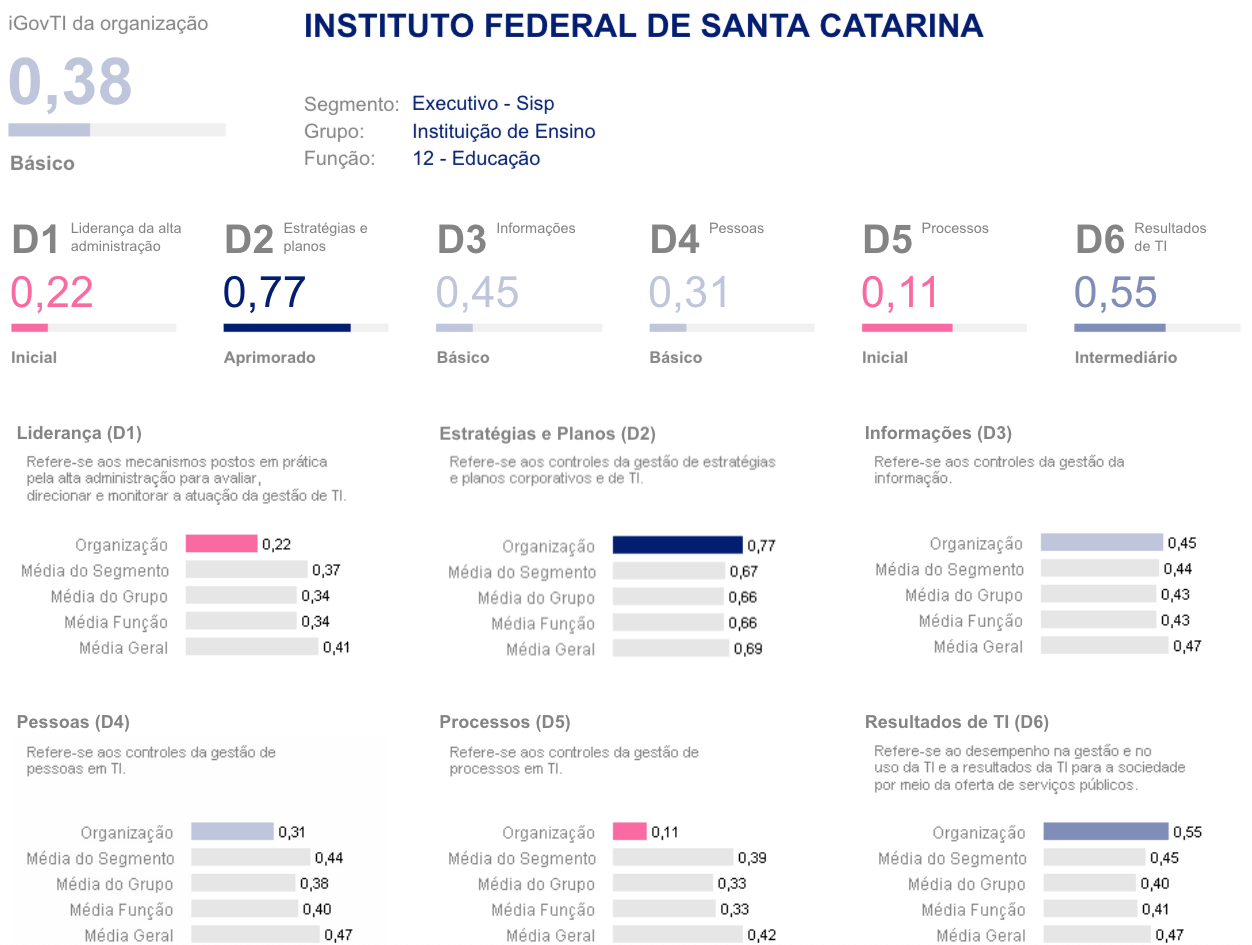
\includegraphics[angle=90,width=16cm]{TCC/figuras/9.1-anexos/iGovTI-IFSC.png}
    
%     Fonte: \cite{igovti}
% \end{figure}
% % ----------------------------------------------------------
% \chapter{Cálculo iGovTI da UFSC}
% \label{iGovTI_UFSC}
% \begin{figure}[!htpb]
% 	\centering
%     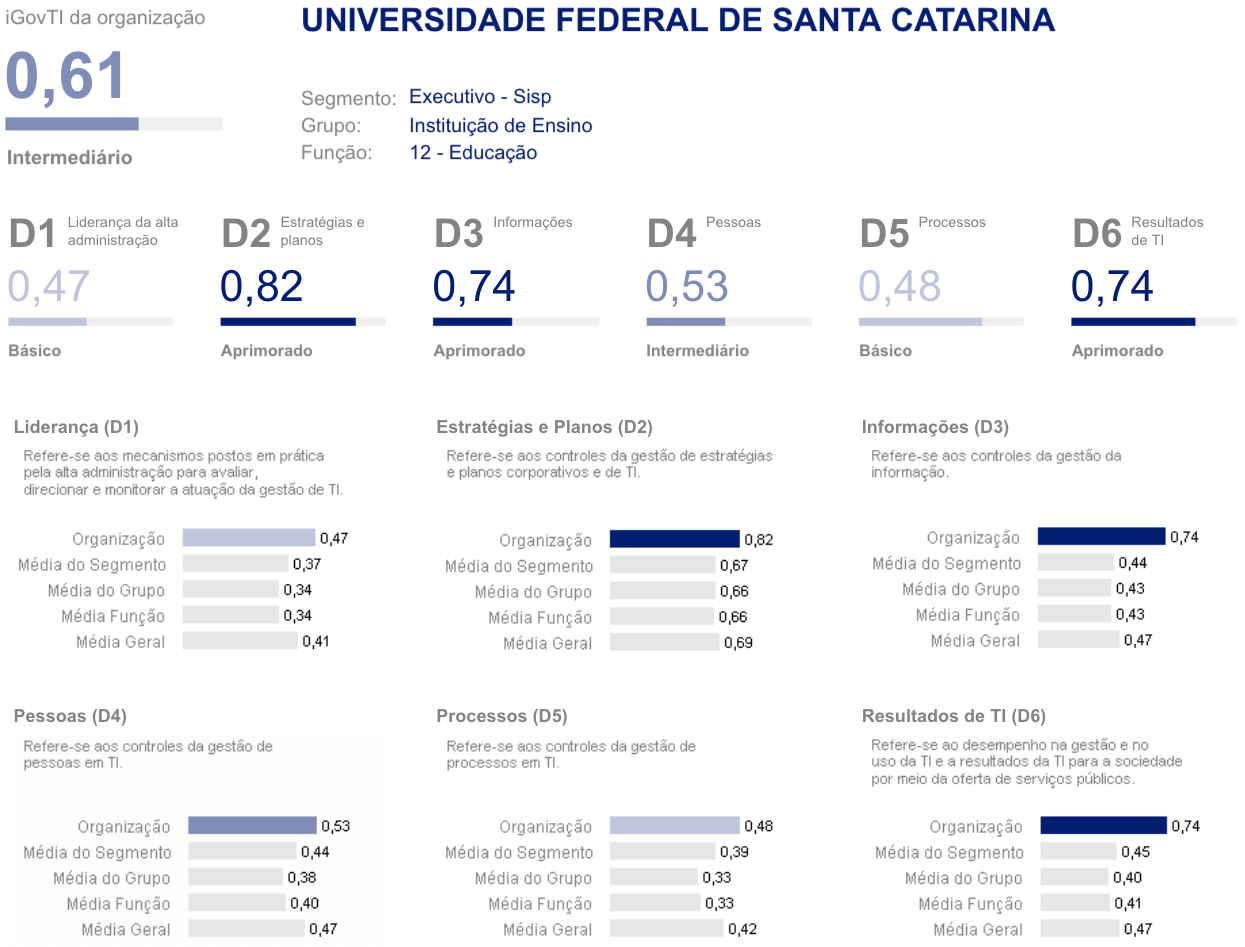
\includegraphics[angle=90,width=16cm]{TCC/figuras/9.1-anexos/iGovTI-UFSC.png}
    
%     Fonte: \cite{igovti}
% \end{figure}
% % ----------------------------------------------------------
\chapter{Instruções de criação do \textit{cluster} Kubernetes}

Arquivo README.md contendo instruções de criação da infraestrutura remota e cluster \textit{Kubernetes}. Disponível em \href{https://goo.gl/aZ3Grb}{https://goo.gl/aZ3Grb}

\begin{figure}[!htpb]
	\centering
    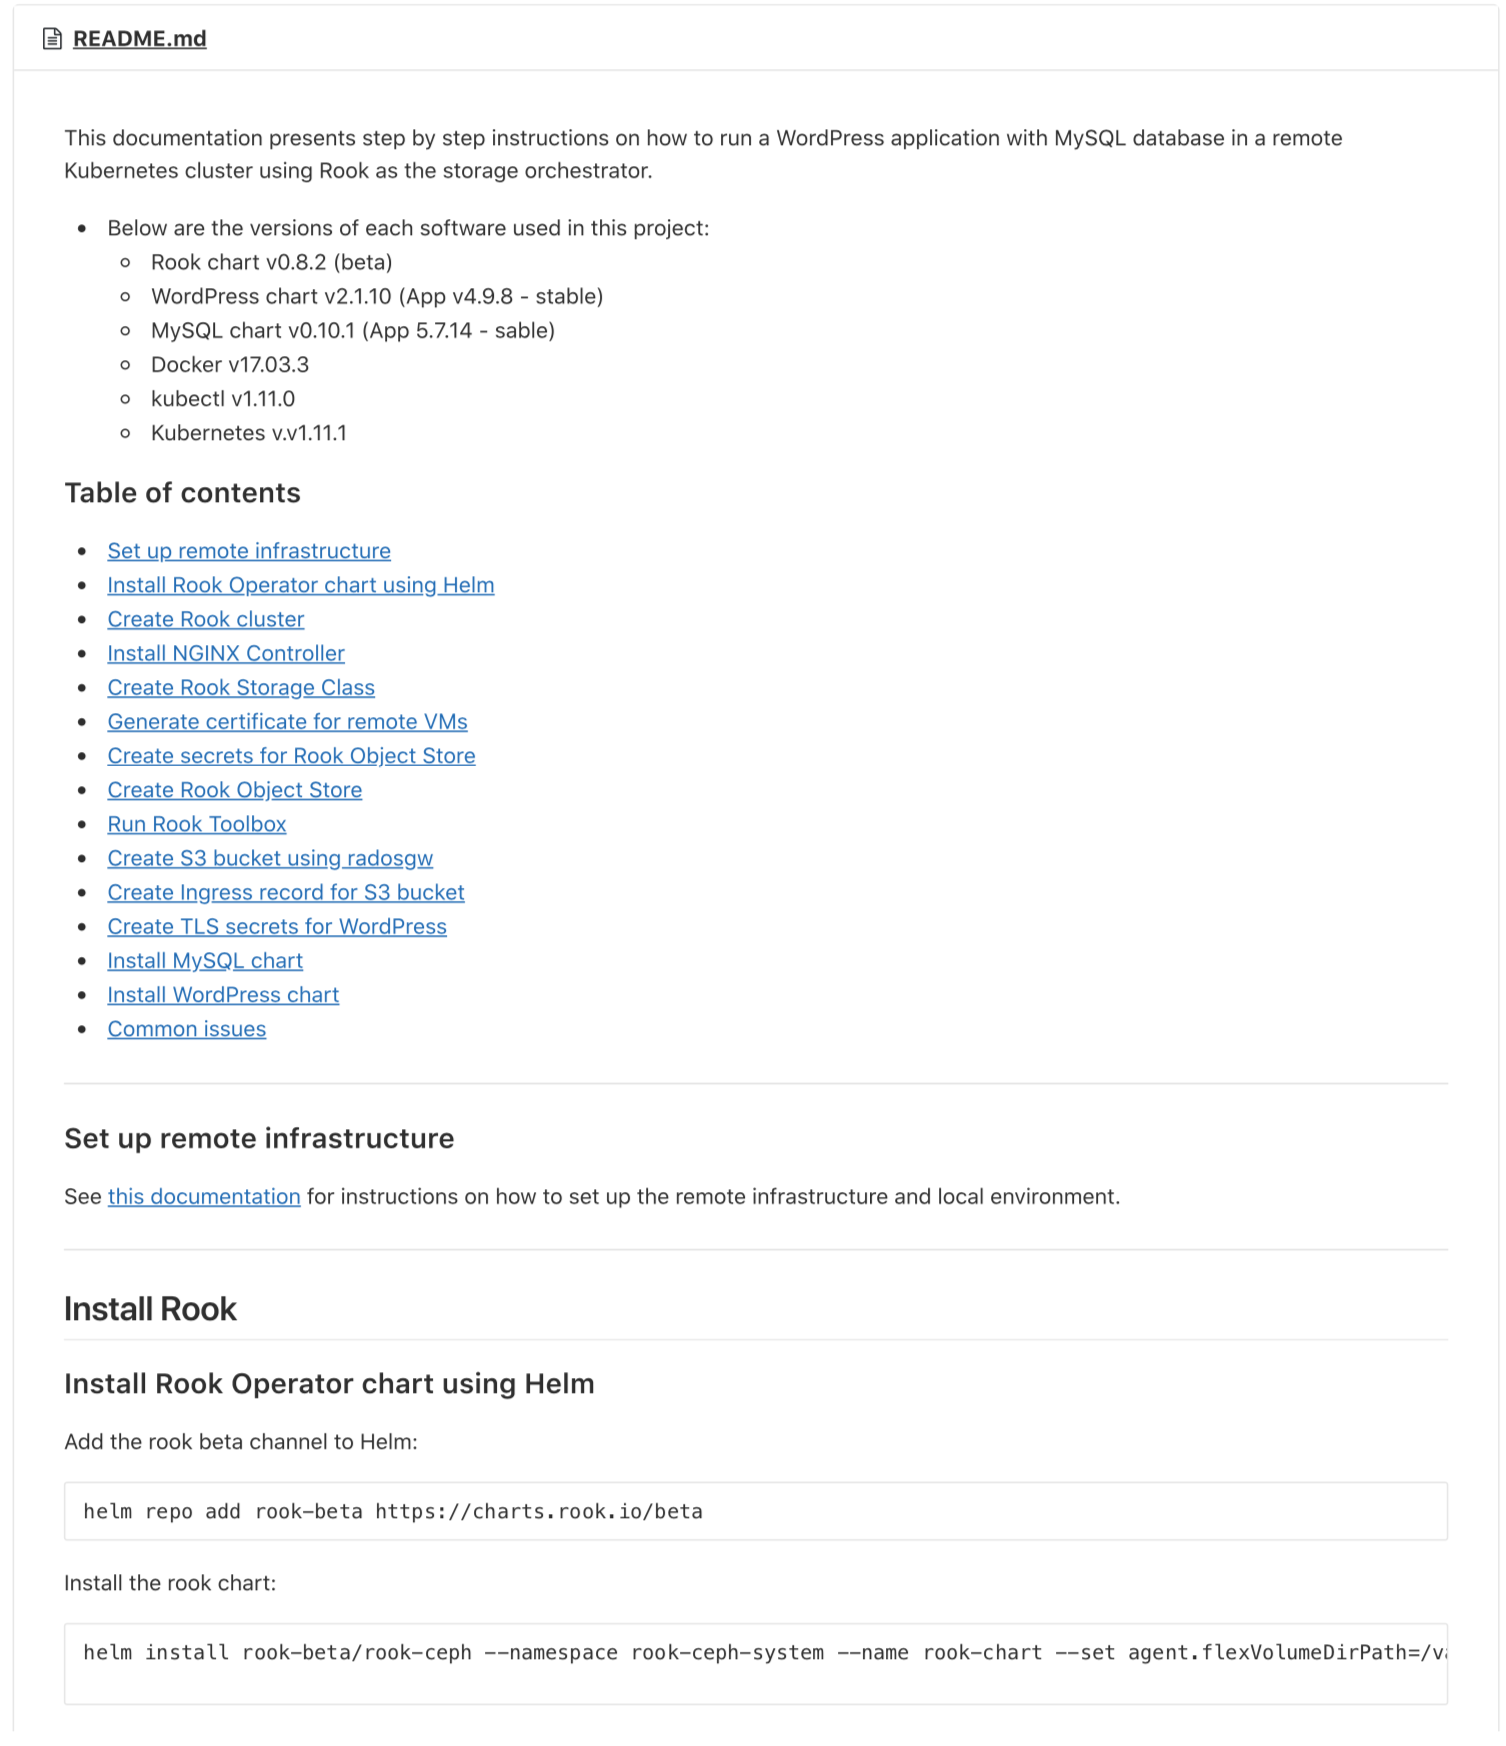
\includegraphics[scale=0.61]{TCC/readmes/remote-setup-readme-1.png}
\end{figure}

\includepdf[scale=0.95,pages=2-3]{TCC/readmes/remote-setup-readme.pdf}
% ----------------------------------------------------------
\chapter{Instruções de implantação do \textit{cluster} Rook}

Arquivo README.md contendo instruções de implantação do \textit{cluster} Rook e aplicações MySQL e WordPress. Disponível em \href{https://goo.gl/Qe1PvX}{https://goo.gl/Qe1PvX}

\begin{figure}[!htpb]
	\centering
    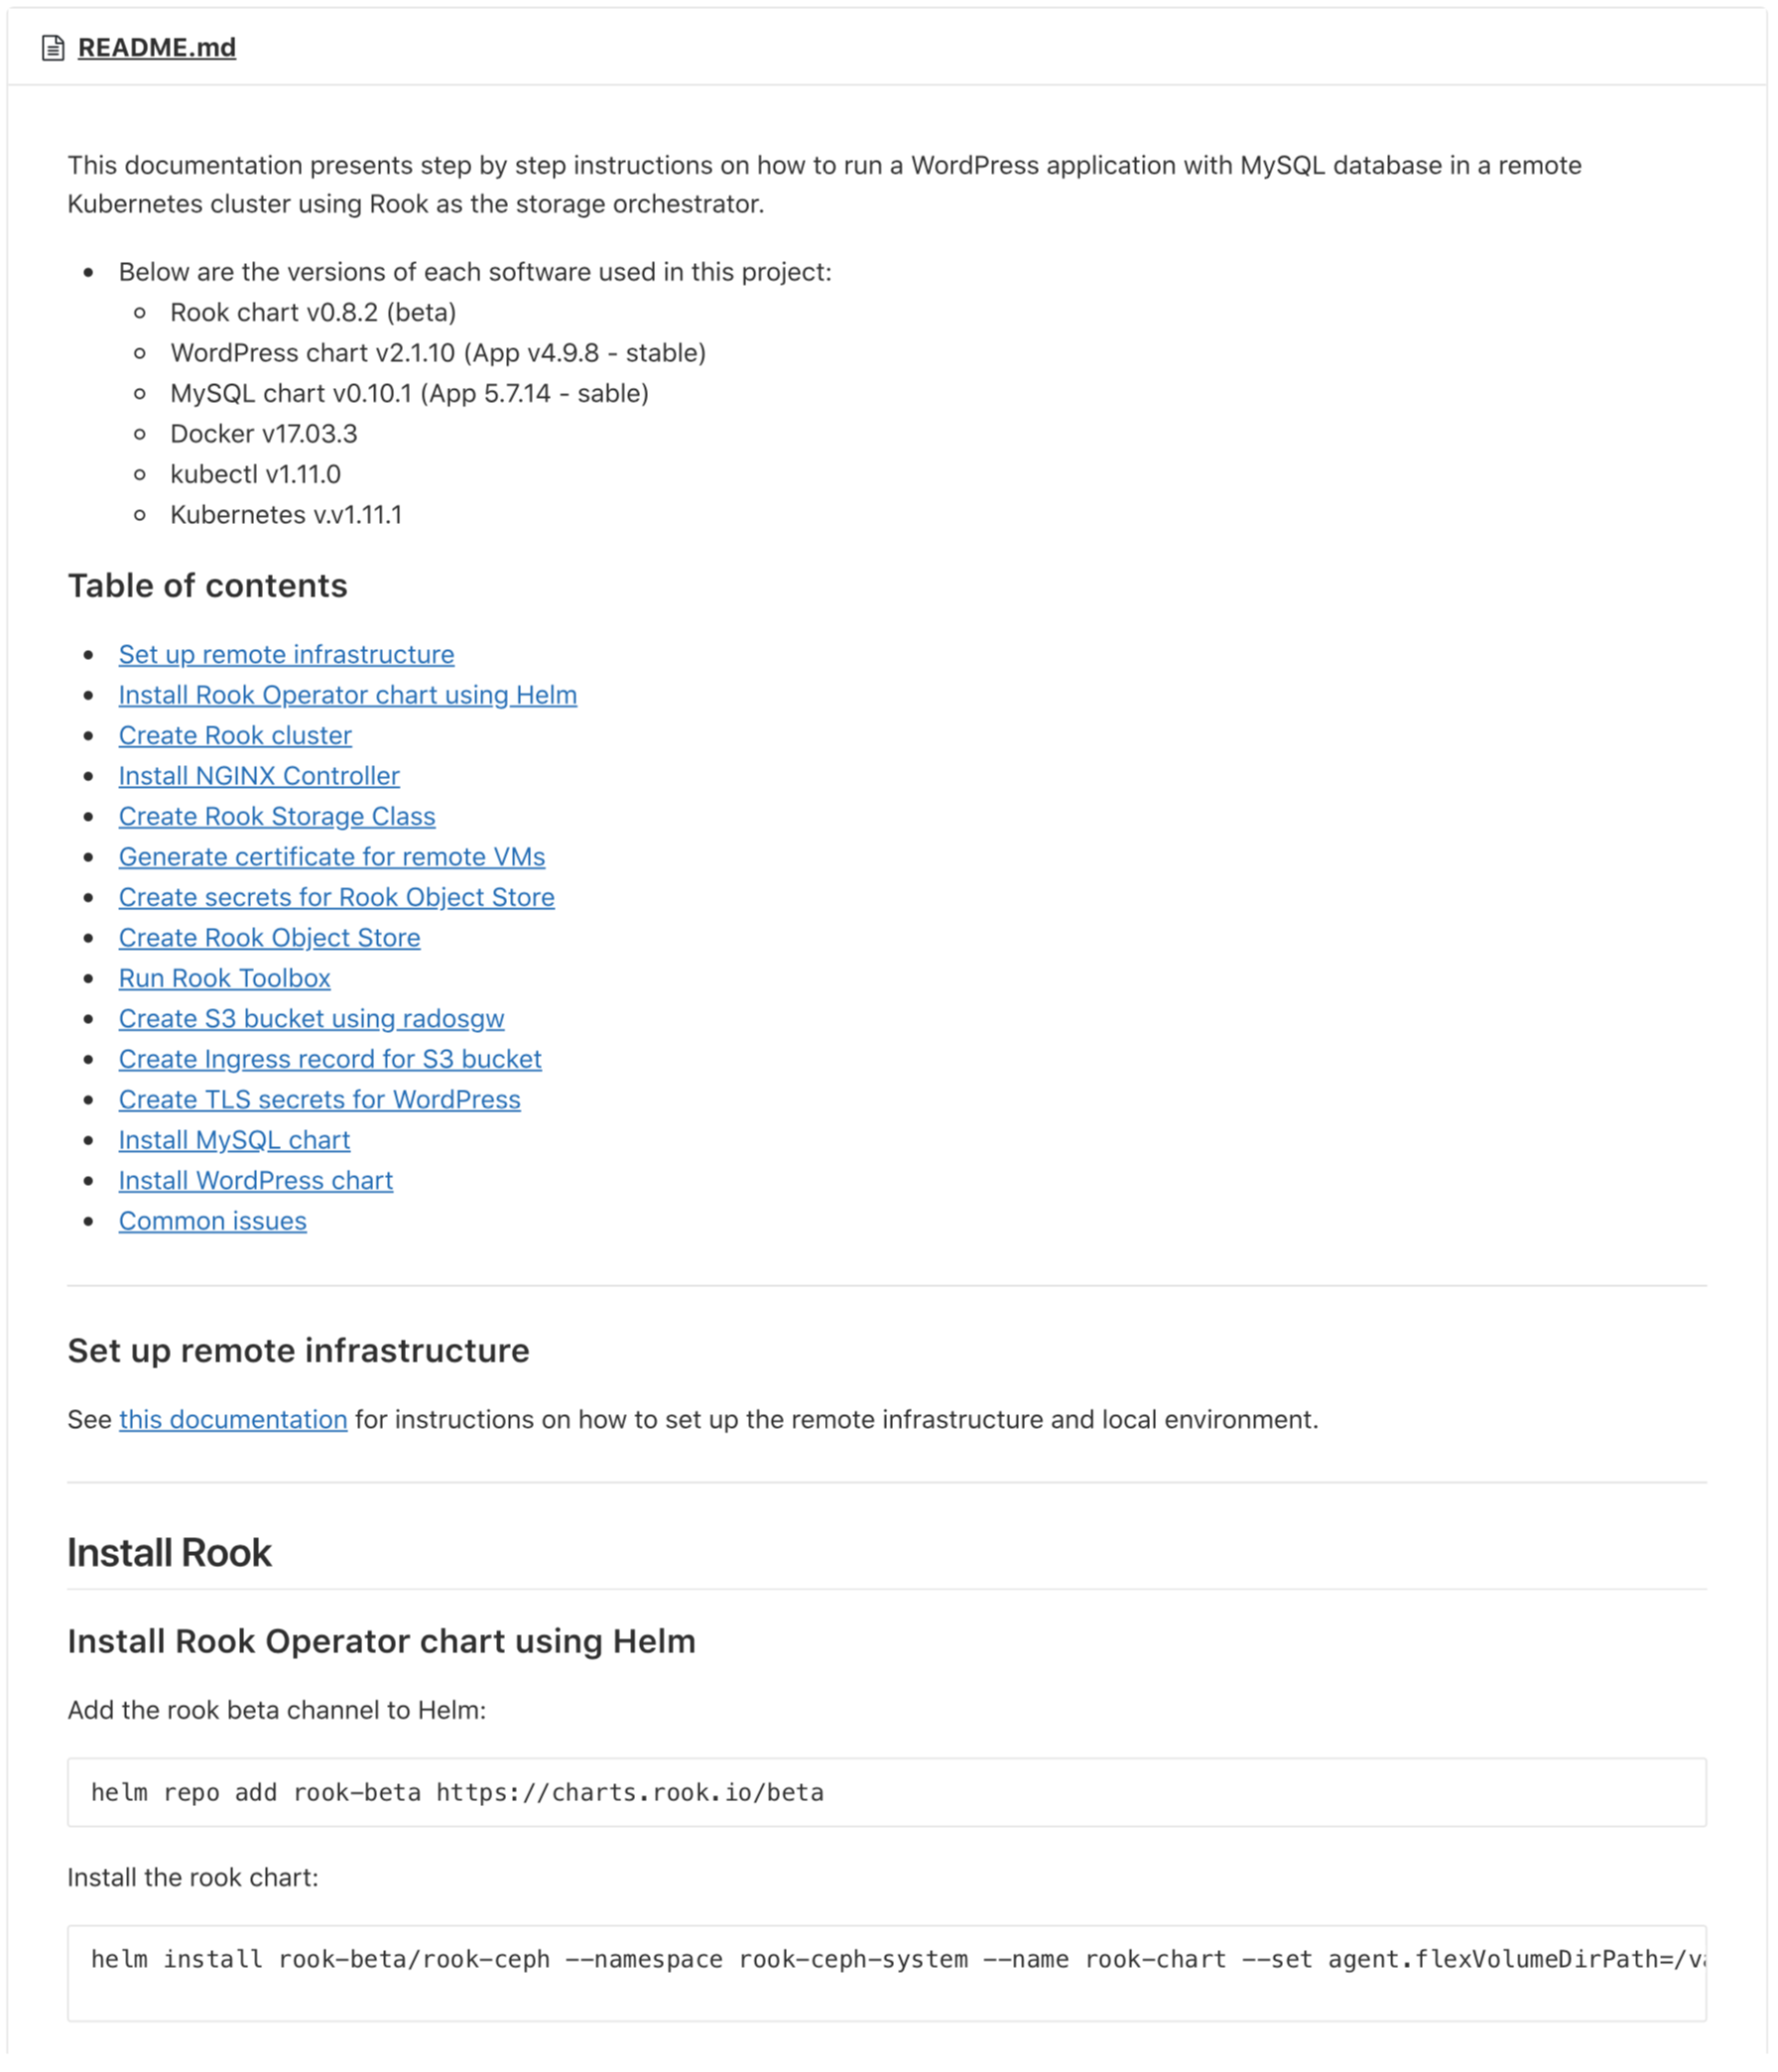
\includegraphics[scale=0.5]{TCC/readmes/k8s-deployment-readme-1.png}
\end{figure}

\includepdf[scale=0.97,pages=2-]{TCC/readmes/k8s-deployment-readme.pdf}
% ----------------------------------------------------------

\end{anexosenv}

%---------------------------------------------------------------------
% INDICE REMISSIVO
%---------------------------------------------------------------------
\phantompart
\printindex
%---------------------------------------------------------------------

\end{document}
